\setchapterpreamble[u]{\margintoc} 
\chapter{Résoudre un problème de cinématique} 
\section{Analyser un mécanisme, justifier des choix des liaisons, réaliser un schéma cinématique paramétré} 
\graphicspath{{\repStyle/png/}{../CIN/CIN-01-ModeliserSchemasCinematiques/01_T/images/}} 
\normaltrue
\correctiontrue

%\UPSTIidClasse{11} % 11 sup, 12 spé
%\newcommand{\UPSTIidClasse}{12}


\exer{Mouvement T -- $\star$ \label{CIN:01:B2:12:01}}
\setcounter{question}{0}\marginnote{\xpComp{CIN}{01}}%\UPSTIcompetence{B2-12}
\index{Compétence B2-12}\index{Compétence CIN-01}
\index{Mécanisme à 1 translation}
\ifcorrection
\else
\marginnote{\textbf{Pas de corrigé pour cet exercice.}}
\fi

\ifprof
\else
Soit le mécanisme suivant. On note $\vect{AB}=\lambda(t)\vect{i_0}$.
\begin{marginfigure}
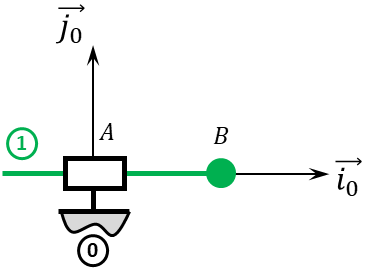
\includegraphics[width=\linewidth]{01_T_01}
\end{marginfigure}
\fi

\question{Tracer le graphe des liaisons.}
\ifprof\begin{marginfigure}
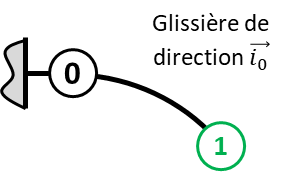
\includegraphics[width=\linewidth]{01_T_01_c}
\end{marginfigure}
\else
\fi


\question{Retracer le schéma cinématique pour $\lambda=\SI{10}{mm}$.}
\ifprof
\begin{marginfigure}
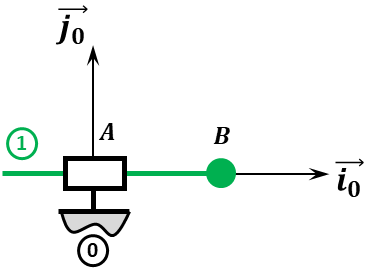
\includegraphics[width=\linewidth]{01_T_02_c}
\end{marginfigure}
\else
\fi

\question{Retracer le schéma cinématique pour $\lambda=-\SI{20}{mm}$.}
\ifprof
\begin{marginfigure}
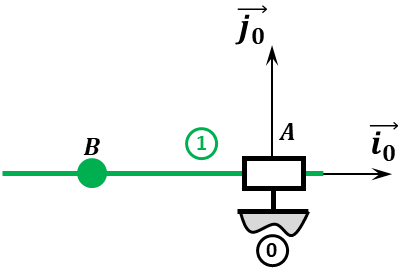
\includegraphics[width=\linewidth]{01_T_03_c}
\end{marginfigure}
\else
\fi

\ifprof
\else
\marginnote{Corrigé  voir \ref{CIN:01:B2:12:01}.}
\fi


 
 
\graphicspath{{\repStyle/png/}{../CIN/CIN-01-ModeliserSchemasCinematiques/02_R/images/}} 
\normaltrue
\correctiontrue

%\UPSTIidClasse{11} % 11 sup, 12 spé
%\newcommand{\UPSTIidClasse}{12}

%\section{Rotation simple} %\label{CIN:01:B2:12:01}
\exer{Mouvement R  $\star$ \label{CIN:01:B2:12:02}}
\setcounter{question}{0}\marginnote{\xpComp{CIN}{01}}%\UPSTIcompetence{B2-12}
\index{Compétence B2-12}\index{Compétence CIN-01}
\index{Mécanisme à 1 rotation}
\ifcorrection
\else
\marginnote{\textbf{Pas de corrigé pour cet exercice.}}
\fi

\ifprof
\else
Soit le mécanisme suivant. On a $\vect{AB}=R\vect{i_1}$ avec $R=\SI{20}{mm}$. 
\begin{marginfigure}
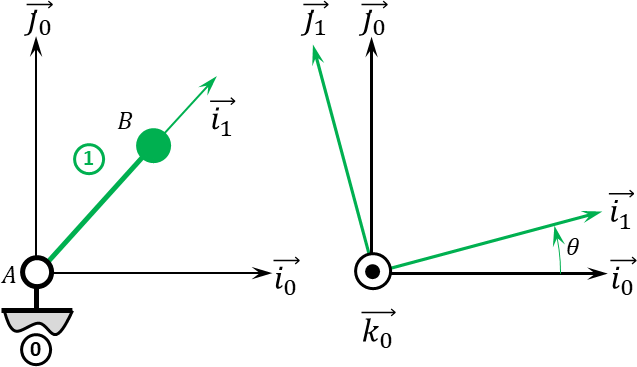
\includegraphics[width=\linewidth]{02_R_01}
\end{marginfigure}
\fi

\ifprof
\begin{multicols}{3}
\else
\fi
\question{Tracer le graphe des liaisons.}
\ifprof
\begin{marginfigure}
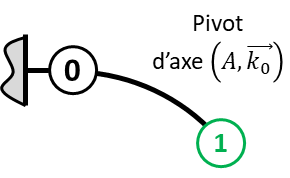
\includegraphics[width=\linewidth]{02_R_01_c}
\end{marginfigure}
\vfill\null
\columnbreak
\else
\fi

\question{Retracer le schéma cinématique pour $\theta=\dfrac{\pi}{4}\,\text{rad}$.}
\ifprof
\begin{marginfigure}
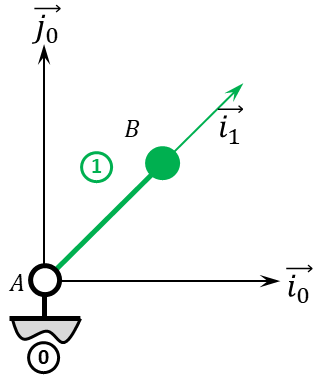
\includegraphics[width=.4\linewidth]{02_R_02_c}
\end{marginfigure}
\vfill\null
\columnbreak
\else
\fi

\question{Retracer le schéma cinématique pour $\theta={\pi}\, \text{rad}$.}
\ifprof
\begin{marginfigure}
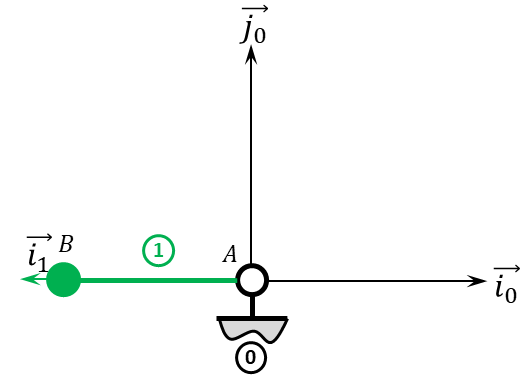
\includegraphics[width=.8\linewidth]{02_R_03_c}
\end{marginfigure}
\else
\fi



\ifprof
\end{multicols}
\else
\fi

\ifprof
\else

\marginnote{Corrigé  voir \ref{CIN:01:B2:12:02}.}

\fi 
 
\graphicspath{{\repStyle/png/}{../CIN/CIN-01-ModeliserSchemasCinematiques/03_TT/images/}} 
\normaltrue
\correctiontrue

%\UPSTIidClasse{11} % 11 sup, 12 spé
%\newcommand{\UPSTIidClasse}{12}


\exer{Mouvement TT -- $\star$ \label{CIN:01:B2:12:03}}
\setcounter{question}{0}\marginnote{\xpComp{CIN}{01}}%\UPSTIcompetence{B2-12}
\index{Compétence B2-12}\index{Compétence CIN-01}
\index{Mécanisme à 2 translations}
\ifcorrection
\else
\marginnote{\textbf{Pas de corrigé pour cet exercice.}}
\fi

\ifprof
\else
Soit le mécanisme suivant. On note $\vect{AB}=\lambda(t)\vect{i_0}$ et $\vect{BC}=\mu(t)\vect{j_0}$.
\begin{marginfigure}
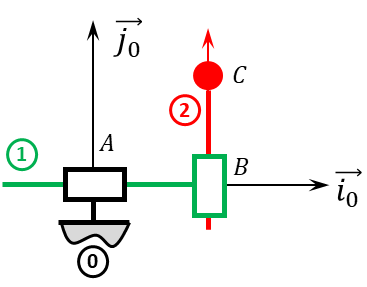
\includegraphics[width=\linewidth]{03_TT_01}
\end{marginfigure}
\fi

\ifprof
\begin{multicols}{3}
\else
\fi
\question{Tracer le graphe des liaisons.}
\ifprof
\begin{marginfigure}
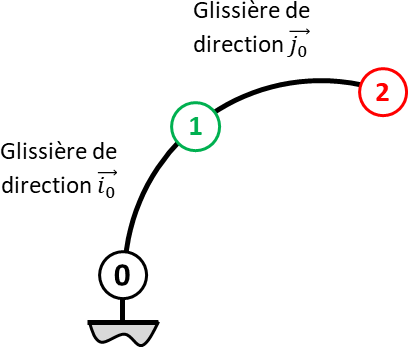
\includegraphics[width=\linewidth]{03_TT_01_c}
\end{marginfigure}
\else
\fi

\question{Retracer le schéma cinématique pour $\lambda=\SI{10}{mm}$ et $\mu=\SI{10}{mm}$.}
\ifprof
\begin{marginfigure}
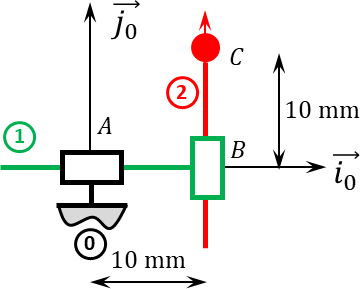
\includegraphics[width=\linewidth]{03_TT_02_c}
\end{marginfigure}
\else
\fi

\question{Retracer le schéma cinématique pour $\lambda=\SI{20}{mm}$ et $\mu=\SI{10}{mm}$.}
\ifprof
\begin{marginfigure}
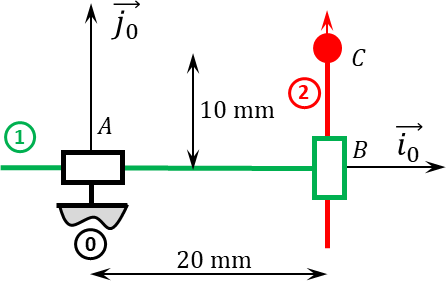
\includegraphics[width=.8\linewidth]{03_TT_03_c}
\end{marginfigure}
\else
\fi


\ifprof
\end{multicols}
\else
\fi

\ifprof
\else

\marginnote{Corrigé  voir \ref{CIN:01:B2:12:03}.}

\fi


 
 
\graphicspath{{\repStyle/png/}{../CIN/CIN-01-ModeliserSchemasCinematiques/04_RR/images/}} 
\normaltrue
\correctiontrue

%\UPSTIidClasse{11} % 11 sup, 12 spé
%\newcommand{\UPSTIidClasse}{12}

\exer{Mouvement RR  $\star$ \label{CIN:01:B2:12:04}}
\setcounter{question}{0}\marginnote{\xpComp{CIN}{01}}%\UPSTIcompetence{B2-12}
\index{Compétence B2-12}\index{Compétence CIN-01}
\index{Mécanisme à 2 rotations}
\ifcorrection
\else
\marginnote{\textbf{Pas de corrigé pour cet exercice.}}
\fi

\ifprof
\else
Soit le mécanisme suivant. On a $\vect{AB}=R\vect{i_1}$ avec $R=\SI{20}{mm}$ et  
$\vect{BC}=L\vect{i_2}$ avec $L=\SI{15}{mm}$.
\begin{marginfigure}
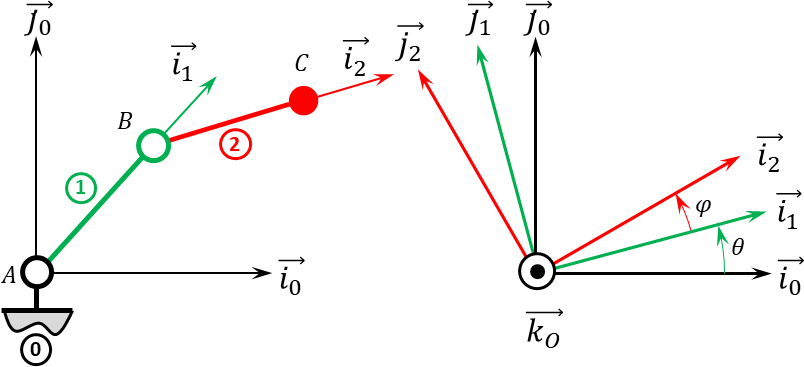
\includegraphics[width=\linewidth]{04_RR_01}
\end{marginfigure}
\fi

\question{Tracer le graphe des liaisons.}
\ifprof
\begin{marginfigure}
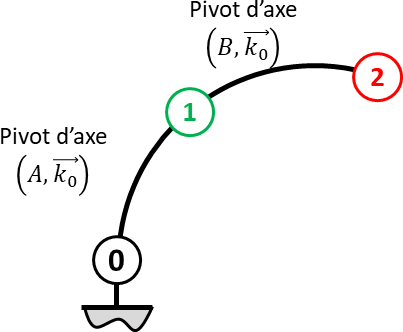
\includegraphics[width=.2\linewidth]{04_RR_01_c}
\end{marginfigure}
\else
\fi


\ifprof
\begin{multicols}{3}
\else
\fi

\question{Retracer le schéma cinématique pour $\theta=\dfrac{\pi}{4}\,\text{rad}$ et $\varphi=\pi\,\text{rad}$.}
\ifprof
\begin{marginfigure}
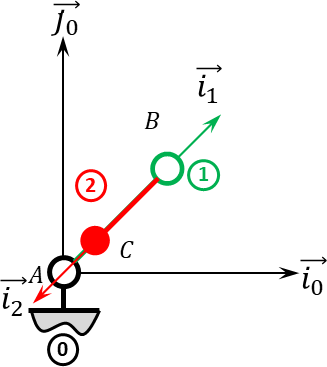
\includegraphics[width=\linewidth]{04_RR_02_c}
\end{marginfigure}
\else
\fi

\question{Retracer le schéma cinématique pour $\theta=\dfrac{\pi}{4}\,\text{rad}$ et $\varphi=-\dfrac{\pi}{4}\,\text{rad}$.}
\ifprof
\begin{marginfigure}
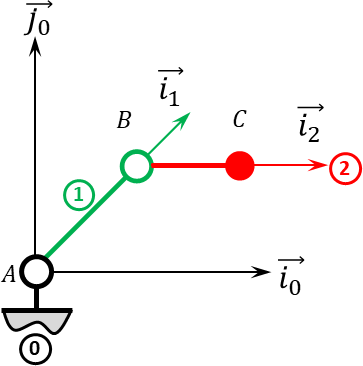
\includegraphics[width=\linewidth]{04_RR_03_c}
\end{marginfigure}
\else
\fi


\question{Retracer le schéma cinématique pour $\theta=\dfrac{3\pi}{4}\,\text{rad}$ et $\varphi=-\dfrac{\pi}{4}\,\text{rad}$.}
\ifprof
\begin{marginfigure}
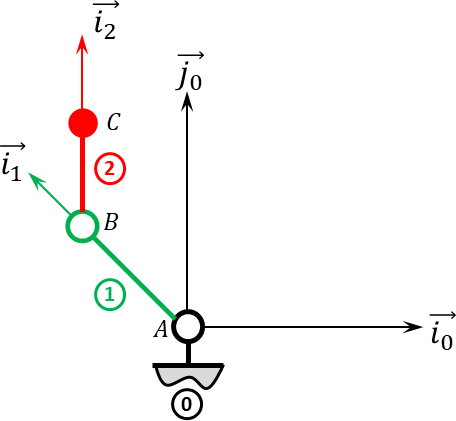
\includegraphics[width=\linewidth]{04_RR_04_c}
\end{marginfigure}
\else
\fi

\ifprof
\end{multicols}
\else
\fi

\ifprof
\else

\marginnote{Corrigé  voir \ref{CIN:01:B2:12:04}.}

\fi 
 
\graphicspath{{\repStyle/png/}{../CIN/CIN-01-ModeliserSchemasCinematiques/05_RT/images/}} 
\normaltrue
\correctiontrue

%\UPSTIidClasse{11} % 11 sup, 12 spé
%\newcommand{\UPSTIidClasse}{12}

\exer{Mouvement RT  $\star$ \label{CIN:01:B2:12:05}}
\setcounter{question}{0}\marginnote{\xpComp{CIN}{01}}%\UPSTIcompetence{B2-12}
\index{Compétence B2-12}\index{Compétence CIN-01}
\index{Mécanisme à 1 rotation et 1 translation}
\ifcorrection
\else
\marginnote{\textbf{Pas de corrigé pour cet exercice.}}
\fi

\ifprof
\else
Soit le mécanisme suivant. On a $\vect{AB}=\lambda(t)\vect{i_1}$.
\begin{marginfigure}
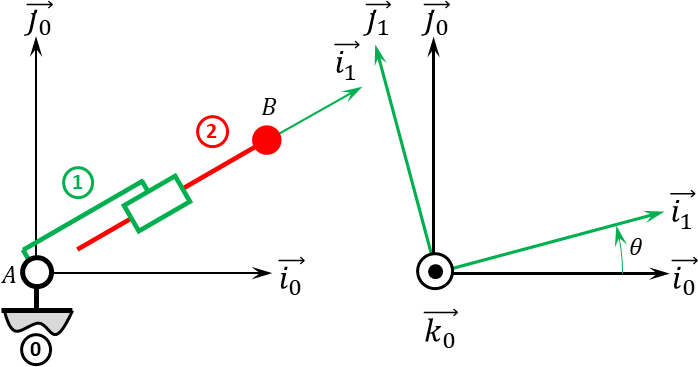
\includegraphics[width=\linewidth]{05_RT_01}
\end{marginfigure}
\fi

\question{Tracer le graphe des liaisons.}
\ifprof
\begin{marginfigure}
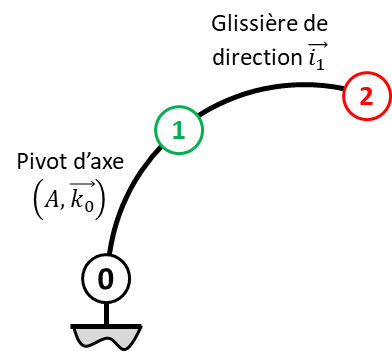
\includegraphics[width=\linewidth]{05_RT_01_01}
\end{marginfigure}
\else
\fi

\question{Retracer le schéma cinématique pour $\theta=\dfrac{\pi}{4}\,\text{rad}$ et $\lambda(t)=\SI{20}{mm}$.}
\ifprof
\else
\fi

\question{Retracer le schéma cinématique pour $\theta=\dfrac{-\pi}{4}\,\text{rad}$ et $\lambda(t)=-\SI{20}{mm}$.}
\ifprof\begin{marginfigure}
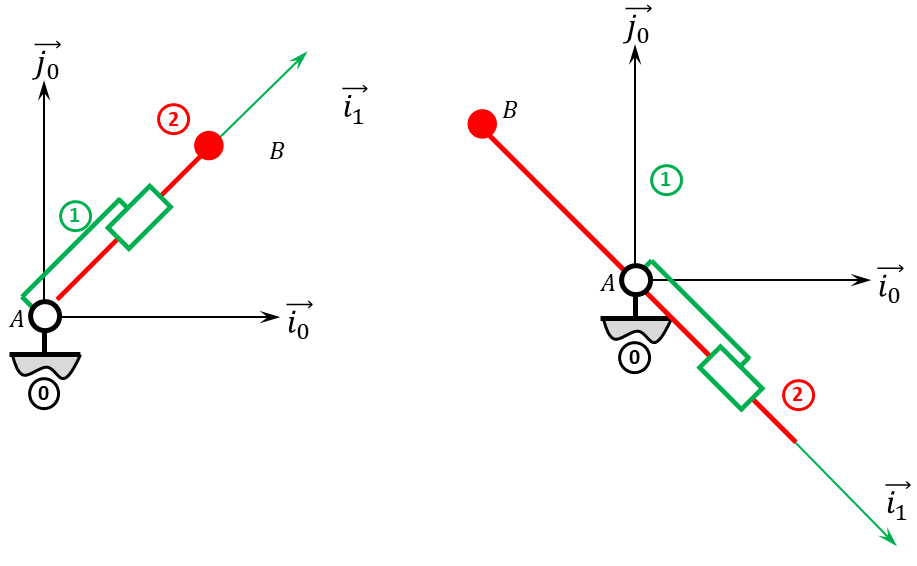
\includegraphics[width=.8\linewidth]{05_RT_01_02}
\end{marginfigure}
\else
\fi




\ifprof
\else

\marginnote{Corrigé  voir \ref{CIN:01:B2:12:05}.}

\fi 
 
\graphicspath{{\repStyle/png/}{../CIN/CIN-01-ModeliserSchemasCinematiques/06_TR/images/}} 
\normaltrue
\correctionfalse

%\UPSTIidClasse{11} % 11 sup, 12 spé
%\newcommand{\UPSTIidClasse}{12}

\exer{Mouvement RT  $\star$ \label{CIN:01:B2:12:06}}
\setcounter{question}{0}\marginnote{\xpComp{CIN}{01}}%\UPSTIcompetence{B2-12}
\index{Compétence B2-12}\index{Compétence CIN-01}
\index{Mécanisme à 1 translation et 1 rotation}
\ifcorrection
\else
\marginnote{\textbf{Pas de corrigé pour cet exercice.}}
\fi

\ifprof
\else
Soit le mécanisme suivant. On a $\vect{AB}=\lambda(t)\vect{i_0}$ et $\vect{BC}=R\vect{i2}$.
\begin{marginfigure}
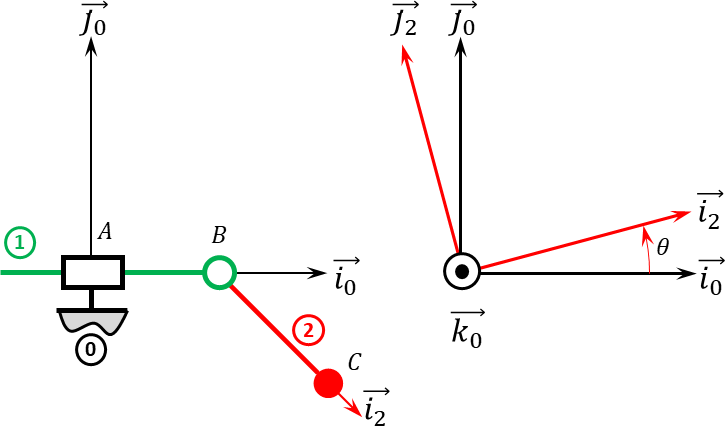
\includegraphics[width=\linewidth]{06_TR_01}
\end{marginfigure}
\fi

\question{Tracer le graphe des liaisons.}
\ifprof
\else
\fi

\question{Retracer le schéma cinématique pour $\theta=\dfrac{\pi}{4}\,\text{rad}$ et $\lambda(t)=\SI{20}{mm}$.}
\ifprof
\else
\fi

\question{Retracer le schéma cinématique pour $\theta=\dfrac{-\pi}{4}\,\text{rad}$ et $\lambda(t)=-\SI{20}{mm}$.}
\ifprof
\else
\fi



\ifprof
\else

\marginnote{Corrigé  voir \ref{CIN:01:B2:12:06}.}

\fi 
 
\graphicspath{{\repStyle/png/}{../CIN/CIN-01-ModeliserSchemasCinematiques/07_RR3D/images/}} 
\normalfalse \difficiletrue \tdifficilefalse
\correctionfalse

%\UPSTIidClasse{11} % 11 sup, 12 spé
%\newcommand{\UPSTIidClasse}{12}

\exer{Mouvement RR 3D  $\star\star$ \label{CIN:01:B2:12:07}}
\setcounter{question}{0}\marginnote{\xpComp{CIN}{01}}%\UPSTIcompetence{B2-12}
\index{Compétence B2-12}\index{Compétence CIN-01}
\index{Mécanisme à 2 rotations 3D}
\ifcorrection
\else
\marginnote{\textbf{Pas de corrigé pour cet exercice.}}
\fi

\ifprof
\else
Soit le mécanisme suivant. On a $\vect{AB}=R\vect{i_1}$ et $\vect{BC}=\ell\vect{i_2}+r\vect{j_2}$. On note $R+\ell=L = \SI{20}{mm}$ et $r=\SI{10}{mm}$.
\begin{marginfigure}
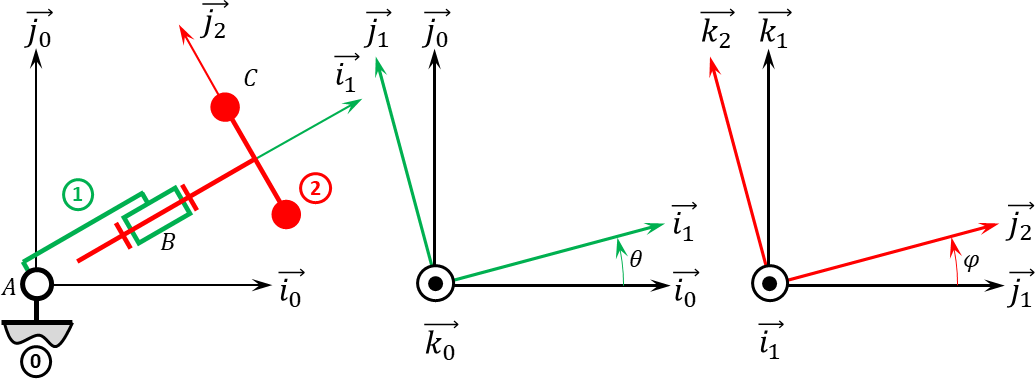
\includegraphics[width=\linewidth]{07_RR3D_01}
\end{marginfigure}
\fi


\question{Tracer le graphe des liaisons.}
\ifprof
\else
\fi

\question{Retracer le schéma cinématique en 3D pour $\theta(t)=\dfrac{\pi}{2}\,\text{rad}$ et $\varphi(t)=\dfrac{\pi}{2}\, \text{rad}$.}
\ifprof
\else
\fi





\ifprof
\else

\marginnote{Corrigé  voir \ref{CIN:01:B2:12:07}.}

\fi 
 
\graphicspath{{\repStyle/png/}{../CIN/CIN-01-ModeliserSchemasCinematiques/08_RR3D/images/}} 
\normalfalse \difficiletrue \tdifficilefalse
\correctionfalse

%\UPSTIidClasse{11} % 11 sup, 12 spé
%\newcommand{\UPSTIidClasse}{12}

\exer{Mouvement RR 3D  $\star\star$ \label{CIN:01:B2:12:08}}
\setcounter{question}{0}\marginnote{\xpComp{CIN}{01}}%\UPSTIcompetence{B2-12}
\index{Compétence B2-12}\index{Compétence CIN-01}
\index{Mécanisme à 2 rotations 3D}
\ifcorrection
\else
\marginnote{\textbf{Pas de corrigé pour cet exercice.}}
\fi

\ifprof
\else
Soit le mécanisme suivant. On a $\vect{AB}=H\vect{j_1}+R\vect{i_1}$ et $\vect{BC}=L\vect{i_2}$. On a $H=\SI{20}{mm}$, $r=\SI{5}{mm}$, $L=\SI{10}{mm}$. 
\begin{marginfigure}
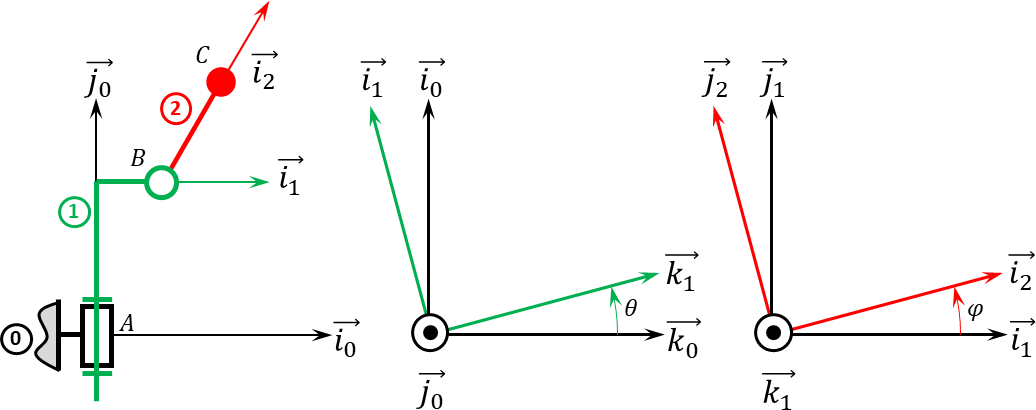
\includegraphics[width=\linewidth]{08_RR3D_01}
\end{marginfigure}
\fi

\question{Tracer le graphe des liaisons.}
\ifprof
\else
\fi

\question{Retracer le schéma cinématique en 3D pour $\theta(t)=\pi\,\text{rad}$ et $\varphi(t)=-\dfrac{\pi}{4}\, \text{rad}$.}
\ifprof
\else
\fi





\ifprof
\else

\marginnote{Corrigé  voir \ref{CIN:01:B2:12:08}.}

\fi 
 
\graphicspath{{\repStyle/png/}{../CIN/CIN-01-ModeliserSchemasCinematiques/09_RT_RSG/images/}} 
\normalfalse \difficiletrue \tdifficilefalse
\correctionfalse

%\UPSTIidClasse{11} % 11 sup, 12 spé
%\newcommand{\UPSTIidClasse}{12}

\exer{Mouvement RT -- RSG  $\star\star$ \label{CIN:01:B2:12:09}}
\setcounter{question}{0}\marginnote{\xpComp{CIN}{01}}%\UPSTIcompetence{B2-12}
\index{Compétence B2-12}\index{Compétence CIN-01}
\index{Mécanisme à 1 rotations, 1 translation et RSG}
\ifcorrection
\else
\marginnote{\textbf{Pas de corrigé pour cet exercice.}}
\fi

\ifprof
\else
Soit le mécanisme suivant. On a $\vect{IA}=R\vect{j_0}$ et $\vect{AB}=\lambda(t)\vect{i_1}$. De plus $R=\SI{15}{mm}$.
\begin{marginfigure}
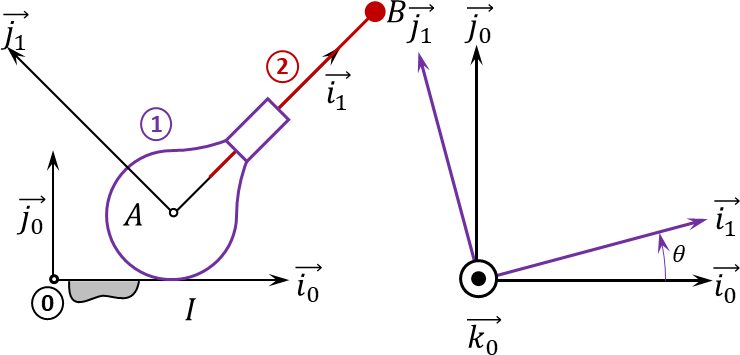
\includegraphics[width=\linewidth]{09_RT_RSG_01}
\end{marginfigure}
\fi


\question{Tracer le graphe des liaisons.}
\ifprof
\else
\fi


\question{Retracer le schéma cinématique pour $\theta(t)=0\,\text{rad}$ et $\lambda(t)=\SI{20}{mm}$. On notera $I_1$ le point de contact entre \textbf{0} et \textbf{1}.}
\ifprof
\else
\fi

\question{Retracer le schéma cinématique pour $\theta(t)=\dfrac{\pi}{2}\,\text{rad}$ et $\lambda(t)=\SI{30}{mm}$. On notera $I_2$ le point de contact entre \textbf{0} et \textbf{1}. On précisera la position des points $I_{0,0}$ et $I_{0,1}$, points résultants de la rupture de contact lors du passage de $\theta(t)$ de 0 à $\dfrac{\pi}{2}$.}
\ifprof
\else
\fi





\ifprof
\else

\marginnote{Corrigé  voir \ref{CIN:01:B2:12:09}.}

\fi 
 
\graphicspath{{\repStyle/png/}{../CIN/CIN-01-ModeliserSchemasCinematiques/1018_BorneReglable/images/}} 
\normalfalse \difficiletrue \tdifficilefalse
\correctionfalse
%\UPSTIidClasse{11} % 11 sup, 12 spé
%\newcommand{\UPSTIidClasse}{12}

\exer{Borne réglable  $\star\star$ \label{CIN:01:B2:12:1018}}
\setcounter{question}{0}\marginnote{\xpComp{CIN}{01}}%\UPSTIcompetence{B2-12}
\index{Compétence B2-12}\index{Compétence CIN-01}
\index{Schéma cinématique}

\ifcorrection
\else
\marginnote{\textbf{Pas de corrigé pour cet exercice.}}
\fi

\ifprof
\else
Soit la borne réglable suivante. 
\begin{marginfigure}
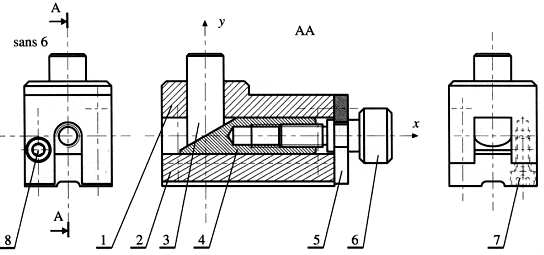
\includegraphics[width=\linewidth]{1018_01}
\end{marginfigure}
\fi


\ifprof
\else
La nomenclature est la suivante. 

\begin{marginfigure}
\begin{tabular}{lll}
\hline
\textbf{Rep} & \textbf{Désignation} & \textbf{Quantité} \\ \hline 
1 & Coulisseau & 1 \\ 
2 & Borne & 1 \\ 
3 & Corps & 1 \\ 
4 & Vis de guidage & 1 \\ 
5 & Couvercle & 1 \\ 
6 & Vis de couvercle & 2 \\ 
7 & Socle & 1 \\ 
8 & Vis de socle & 4 \\ 
10 & Molette & 1 \\ 
12 & Vis & 1 \\
13 & Goupille fendue & 1 \\ 
\hline
\end{tabular}
\end{marginfigure}
\fi


\question{Colorier le dessin de définition en utilisant la même couleur pour une même classe d'équivalence.}
\ifprof
\else
\fi

\question{Lister les classes classes d'équivalence.}
\ifprof
\else
\fi

\question{Donner le graphe de liaisons en précisant rigoureusement les liaisons. Justifier le choix des liaisons.}
\ifprof
\else
\fi


\question{Réaliser le schéma cinématique.}
\ifprof
\else
\fi

\ifprof
\else

\footnotesize
%\begin{marginfigure}
%\begin{tabular}{|p{.9\linewidth}|}
%\hline
%Indications (à vérifier...) :
%\begin{enumerate}
%\item $\vectv{B}{2}{0} = L\varphip(t)\vj{2} +\thetap(t)\left(L\vj{1}-R\vi{0}\right) $.
%\item  $\torseurcin{V}{2}{0} = \torseurl{\vecto{2}{0}=\left( \varphip(t)+\thetap(t) \right) \vk{0} }{ L\varphip(t)\vj{2} +\thetap(t)\left(L\vj{1}-R\vi{0}\right)}{B}$.
%\item $\vectg{B}{2}{0} =  L\varphipp(t)\vj{2}-L\varphip(t)\left(\varphip(t)+\thetap(t) \right)\vi{2}  + \thetapp(t)\left(L\vj{1}-R\vi{0}\right) - L\thetap^2(t)\vi{1}$.
%\end{enumerate} \\ \hline
%\end{tabular}
%\end{marginfigure}
\normalsize



\marginnote{Corrigé  voir \ref{CIN:01:B2:12:1018}.}

\fi 
 
\graphicspath{{\repStyle/png/}{../CIN/CIN-01-ModeliserSchemasCinematiques/1019_RobotPeinture/images/}} 
\normalfalse \difficiletrue \tdifficilefalse
\correctionfalse
%\UPSTIidClasse{11} % 11 sup, 12 spé
%\newcommand{\UPSTIidClasse}{12}

\exer{Robot de toit  $\star\star$ \label{CIN:01:B2:12:1019}}
\setcounter{question}{0}\marginnote{\xpComp{CIN}{01}}%\UPSTIcompetence{B2-12}
\index{Compétence B2-12}\index{Compétence CIN-01}
\index{Schéma cinématique}

\ifcorrection
\else
\marginnote{\textbf{Pas de corrigé pour cet exercice.}}
\fi

\ifprof
\else
Soit le mécanisme donné au verso.
\fi


\ifprof
\else
La nomenclature est la suivante. 
\begin{multicols}{2}
\begin{marginfigure}
\begin{tabular}{|l|l|l|}
\hline
Rep & Nb  & Désignation \\ \hline \hline % & Matière \\ \hline \hline
1 & 1 & Carter inférieur fixe  \\ \hline %&  Al Si 13 \\ \hline 
2&
1&
Carter supérieur pivotant\\ \hline %& Al Si 13 \\ \hline 
3&
2 &
Ecrou hexagonal ISO 4032 - M10 \\ \hline %& \\ \hline 
4&
1&
Rondelle plate ISO 10673 – Type N - 10 \\ \hline %& \\ \hline 
5&
1&
Axe fileté à tête fendu \\ \hline %& \\ \hline 
6&
1&
Plat de fermeture%&
\\ \hline %S 235 \\ \hline 
7&
7&
Rondelle plate ISO 10673 -- Type N - 5 \\ \hline %& \\ \hline 
8&
1&
Bride de liaison support coussinets \\ \hline % &Al Cu 4 Mg Si \\ \hline 
9&
1&
Bride de liaison gauche \\ \hline % & Al Cu 4 Mg Si   \\ \hline 
10&
2&
Coussinet \\ \hline %& Cu Sn 12 P  \\ \hline 
11&
1&
Tube carter \\ \hline %& \\ \hline 
12&
1&
Bride de liaison droite \\ \hline %& Al Cu 4 Mg Si \\ \hline 
13&
1&
Carter cylindrique\\ \hline % & \\ \hline 
14&
1&
Axe excentré \\ \hline %& \\ \hline 
15&
4&
Vis à tête cylindrique à six pans creux\\ \hline % ISO 4762 - M5-50\\ \hline % & \\ \hline 
16&
1&
Chape mâle\\ \hline % & C 45 \\ \hline 
17&
2&
Goupille cylindrique \\ \hline %ISO 8734 - 2x16 \\ \hline %& \\ \hline 
18&
1&
Bielle rotule \\ \hline % &C 45 \\ \hline 
19&
1&
Cale de réglage \\ \hline %& \\ \hline 
20&
1&
Fermeture rotule \\ \hline %& \\ \hline 
21&
1&
Bielle à portée sphérique \\ \hline %& \\ \hline 
22&
3&
Vis à tête cylindrique à six pans creux  \\
&& ISO 4762 - M5-30 \\ \hline %& \\ \hline 
23&
1&
Goupille cylindrique ISO 8734 - 3x30  \\ \hline %& \\ \hline 
24&
1&
Chape femelle \\ \hline %& \\ \hline %C 45 \\ \hline 

25&
1&
Axe de chape \\ \hline % & \\ \hline 
26&
1&
Anneau élastique pour arbre, 4 x 0,4 \\ \hline % & \\ \hline 
27&
2&
Coussinet à collerette \\ \hline %& Cu Sn 12 P \\ \hline 
28&
1&
Bielle \\ \hline % & C 45 \\ \hline 
\end{tabular}
\end{marginfigure}

\begin{marginfigure}
\begin{tabular}{|l|l|l|}
\hline
Rep & Nb  & Désignation \\ \hline \hline % & Matière \\ \hline \hline
29&
3&
Vis à tête cylindrique à six pans creux \\ \hline % ISO 4762 - M5-18 \\ \hline % & \\ \hline 
30&
1&
Axe d'articulation \\ \hline % & \\ \hline 
31&
1&
Axe de sortie \\ \hline % & \\ \hline %100 Cr 6  \\ \hline 
32&
1&
Support d'axe de sortie \\ \hline %C 45 \\ \hline 
33&
1&
Ecrou hexagonal \\ \hline % ISO 4032 - M24  \\ \hline %& \\ \hline 
34&
1&
Rondelle plate \\ \hline % ISO 10673 – Type S - 24\\ \hline % &  \\ \hline 
35&
2&
Coussinet à collerette \\ \hline %& Cu Sn 12 P  \\ \hline 
36&
1&
Plateau support excentrique \\ \hline %& \\ \hline 
37&
1&
Vis à tête moletée \\ \hline %& \\ \hline 
38&
1&
Doigt de réglage \\ \hline % & C 22 \\ \hline 
39&
1&
Coussinet \\ \hline %& Cu Sn 12 P \\ \hline 
40&
1&
Entretoise  \\ \hline 
41&
2&
Anneau élastique pour arbre, 6 x 0,7  \\ \hline %& \\ \hline 
42&
1&
Anneau élastique pour alésage, 32 x 1,5 \\ \hline %& \\ \hline 
43&
1&
Anneau élastique pour arbre, 12 x 1 \\ \hline %& \\ \hline 
44&
1&
Arbre d’entrée \\ \hline %& \\ \hline 
45&
2&
Roulement à une rangée de \\ 
&& billes à contact radial \\ \hline %& \\ \hline 
46&
1&
Support roulements \\ \hline %& Al Cu 4 Mg Si \\ \hline 
47&
1&
Carter \\ \hline % & Al Cu 4 Mg Si \\ \hline 
48&
1&
Vis sans fin Z48 = 2 filets \\ \hline %& \\ \hline 
49&
2&
Boitier\\ \hline % & \\ \hline 
50&
2&
Roulement à une rangée de \\ 
&& billes à contact radial\\  \hline % & \\ \hline 
51&
2&
Joint à deux lèvres \\ \hline %& \\ \hline 
52&
1&
Arbre Creux\\ \hline % & \\ \hline
53&
1&
Vis à tête hexagonale ISO 4014-M6 \\ \hline %  & \\ \hline 
54 & 
1 &
Arbre \\ \hline % & \\ \hline 
55 &
1&
Roue dentée Z55= 60 dents  \\ \hline %&Cu Ni 2 Si  \\ \hline 
\end{tabular}
\end{marginfigure}

\end{multicols}

\fi

\question{Colorier le dessin de définition en utilisant la même couleur pour une même classe d'équivalence.}
\ifprof
\else
\fi

\question{Lister les classes classes d'équivalence.}
\ifprof
\else
\fi

\question{Donner le graphe de liaisons en précisant rigoureusement les liaisons. Justifier le choix des liaisons.}
\ifprof
\else
\fi


\question{Réaliser le schéma cinématique.}
\ifprof
\else
\fi


\ifprof
\else
\begin{marginfigure}
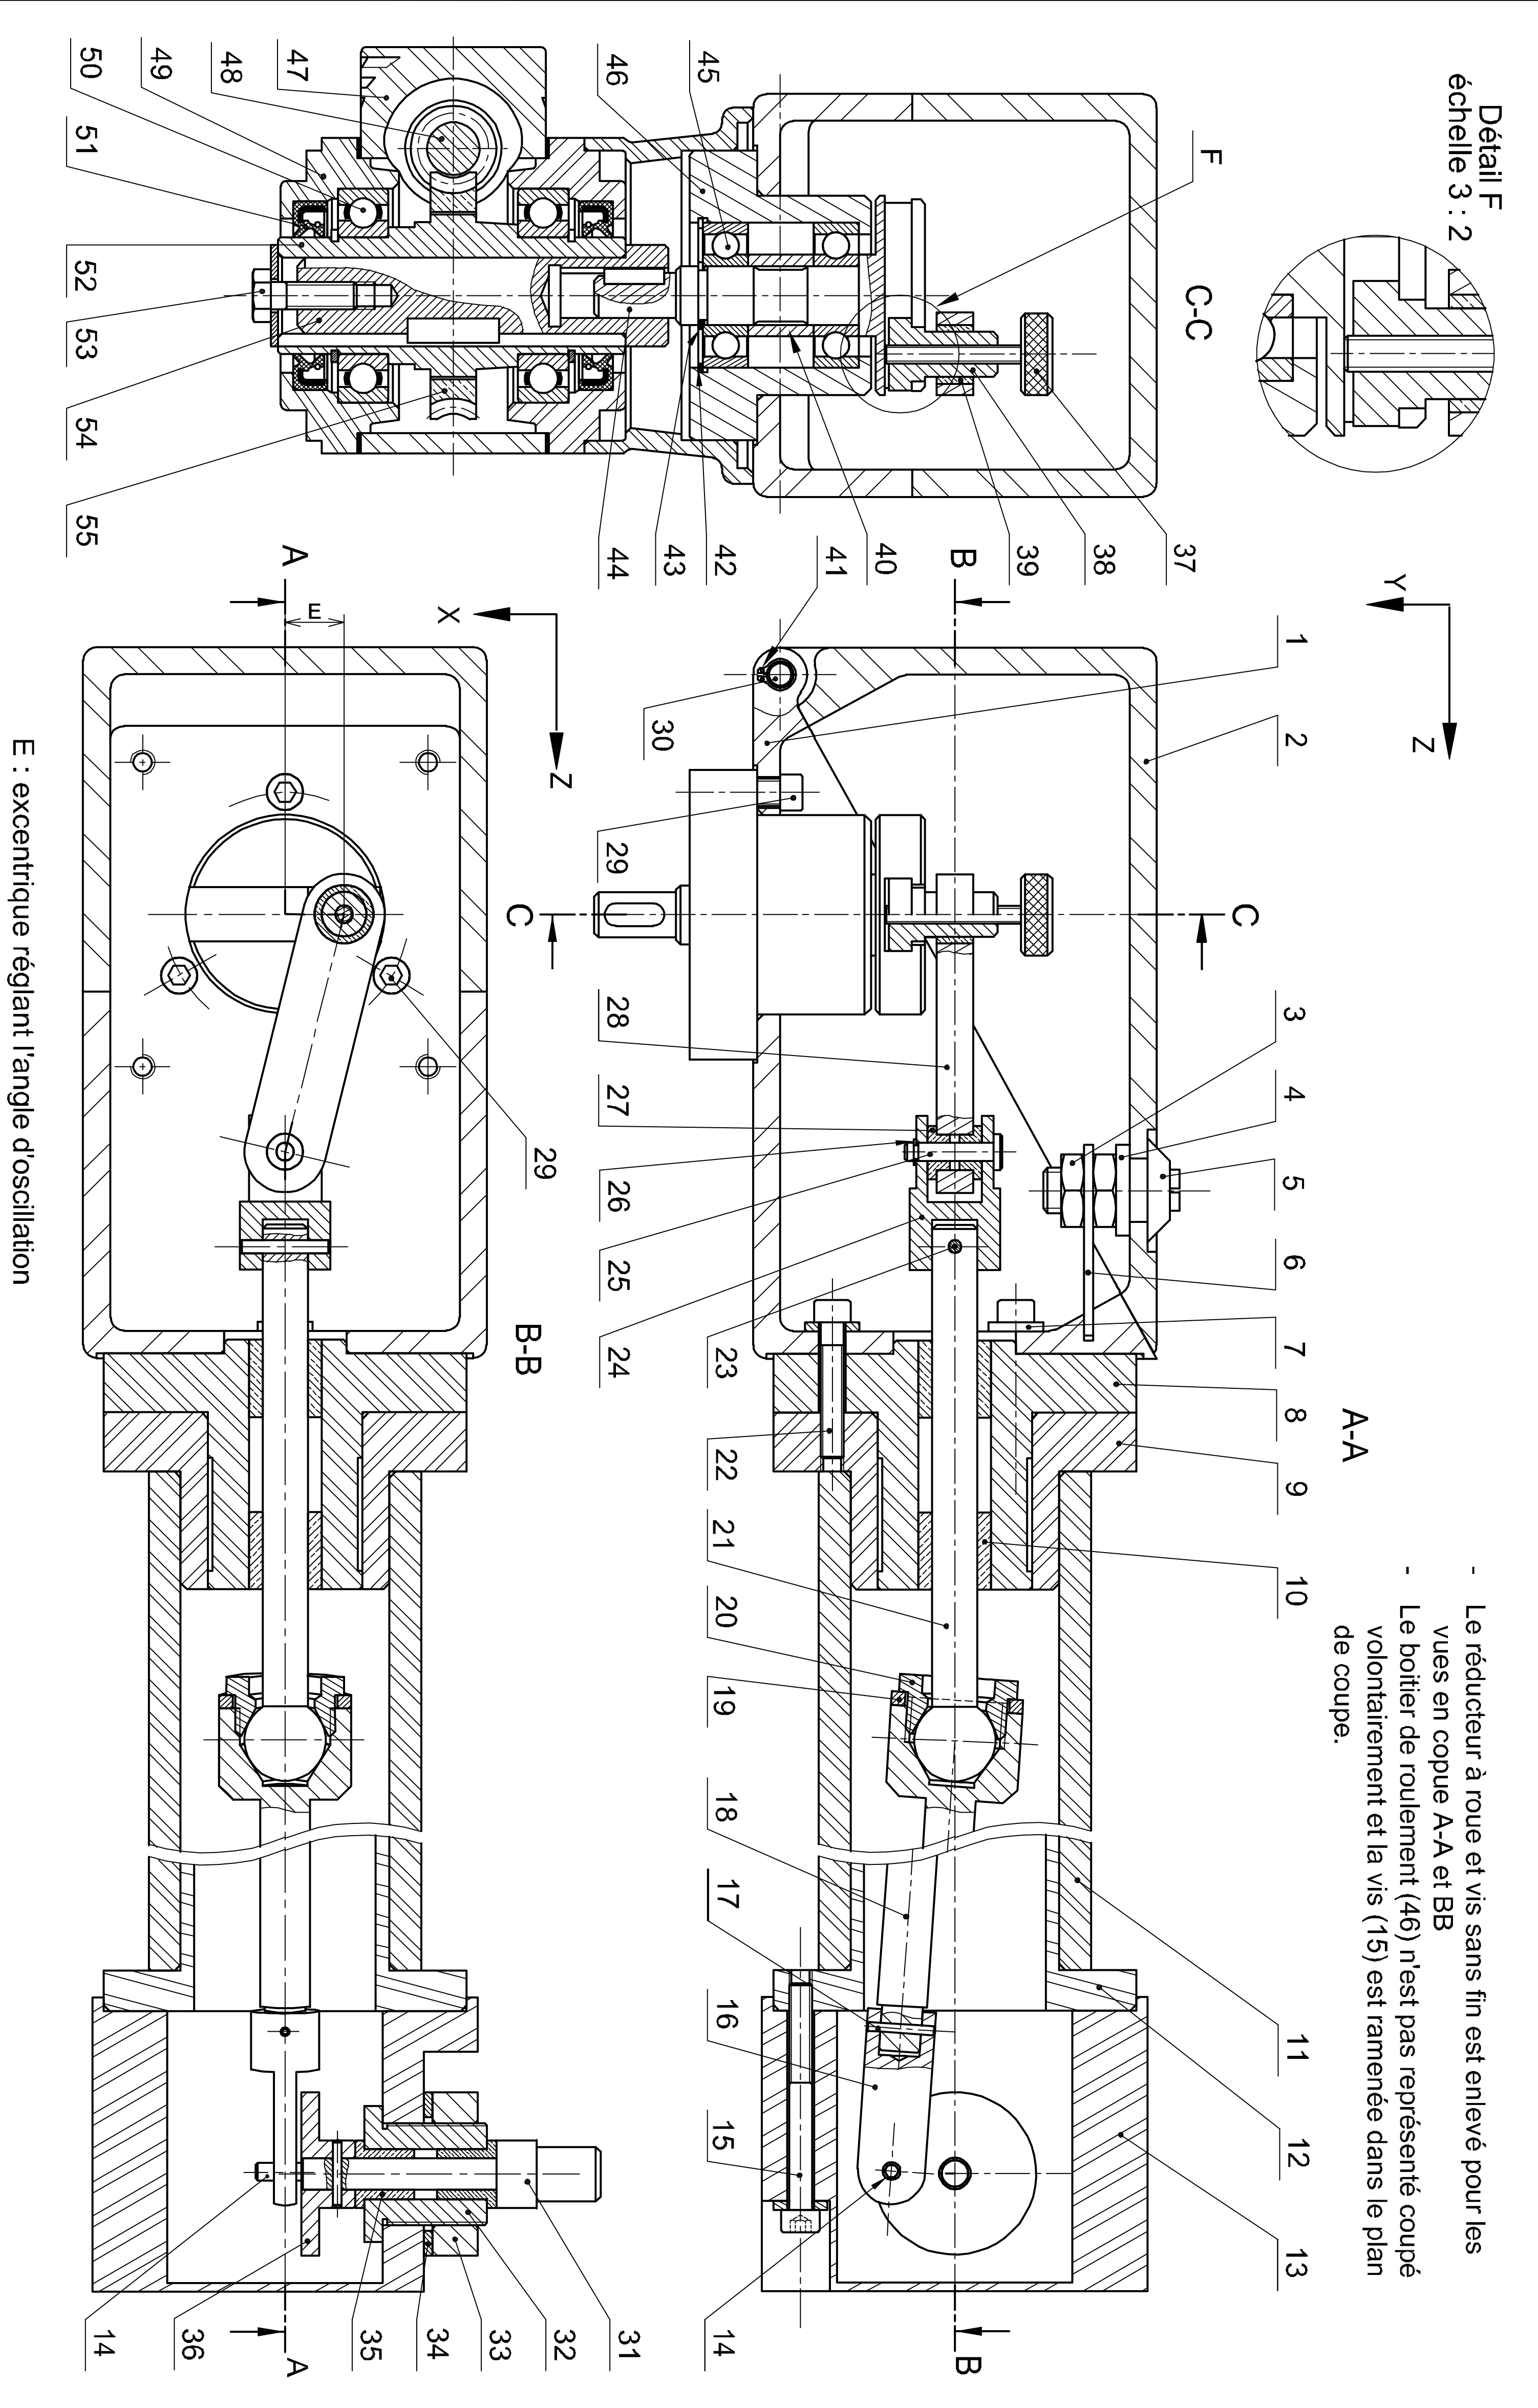
\includegraphics[width=\linewidth]{1019_01}
\end{marginfigure}
\fi


\ifprof
\else

\footnotesize
%\begin{marginfigure}
%\begin{tabular}{|p{.9\linewidth}|}
%\hline
%Indications (à vérifier...) :
%\begin{enumerate}
%\item $\vectv{B}{2}{0} = L\varphip(t)\vj{2} +\thetap(t)\left(L\vj{1}-R\vi{0}\right) $.
%\item  $\torseurcin{V}{2}{0} = \torseurl{\vecto{2}{0}=\left( \varphip(t)+\thetap(t) \right) \vk{0} }{ L\varphip(t)\vj{2} +\thetap(t)\left(L\vj{1}-R\vi{0}\right)}{B}$.
%\item $\vectg{B}{2}{0} =  L\varphipp(t)\vj{2}-L\varphip(t)\left(\varphip(t)+\thetap(t) \right)\vi{2}  + \thetapp(t)\left(L\vj{1}-R\vi{0}\right) - L\thetap^2(t)\vi{1}$.
%\end{enumerate} \\ \hline
%\end{tabular}
%\end{marginfigure}
\normalsize



\marginnote{Corrigé  voir \ref{CIN:01:B2:12:1018}.}

\fi 
 
\graphicspath{{\repStyle/png/}{../CIN/CIN-01-ModeliserSchemasCinematiques/1020_PompeEnsieta/images/}} 
\normalfalse \difficiletrue \tdifficilefalse
\correctionfalse
%\UPSTIidClasse{11} % 11 sup, 12 spé
%\newcommand{\UPSTIidClasse}{12}

\exer{Pompe ENSIETA  $\star\star$ \label{CIN:01:B2:12:1020}}
\setcounter{question}{0}\marginnote{\xpComp{CIN}{01}}%\UPSTIcompetence{B2-12}
\index{Compétence B2-12}\index{Compétence CIN-01}
\index{Schéma cinématique}
\index{Pompe ENSIETA}

\ifcorrection
\else
\marginnote{\textbf{Pas de corrigé pour cet exercice.}}
\fi



\ifprof
\else
Le plan joint format A4 représente l’ensemble monté d’une pompe hydraulique manuelle.

La pompe est fixée sur un support vertical au moyen de 3 trous filetés (1). Une série de trois trous filetés est usinée sur chaque coté du corps (2), permettant ainsi de fixer indifféremment la pompe sur l’une ou l’autre de ses faces.

L’admission de l’huile est effectuée par l’orifice (3), le refoulement par l’orifice (4).

Le pompage s’effectue en actionnant un levier placé dans l’alésage cannelé du maneton (5). Le mouvement alternatif est, par l’intermédiaire de la biellette articulée, transmis au piston coulissant (6).

Lors du mouvement de droite à gauche du piston coulissant, un volume d’huile est aspiré à travers (3) et vient s’emmagasiner dans l’alésage à droite de la tête du piston, simultanément l’huile qui se trouve à gauche de la tête du piston est refoulée par l’orifice (4).

Lors du mouvement de gauche à droite du piston coulissant s’effectue le transfert, à travers de la tête du piston, de l’huile emmagasinée à sa droite (celle-ci passant côté tige). Simultanément une partie de l’huile transférée est refoulée dans (4).

Un clapet anti-retour est constitué d’une bille et d’un ressort. Sur la pompe étudiée ils sont au nombre de trois. 
Le passage du fluide dans un sens, par action sur la bille provoque l’écrasement du ressort et libère le passage. 
Dans le sens contraire l’action du fluide se conjugue avec celle du ressort et interdit le passage. 
\fi

\question{Le diamètre nominal de la bille contenue dans le clapet anti-retour situé sur l’orifice (4) est identique à celui de l’alésage qui la guide. Est-ce fonctionnellement correct ? Justifier votre réponse. L’observation de la pièce (7) du clapet situé sur l’orifice (3) peut vous aider pour la réponse.}

\question{L’alésage du corps contenant l’extrémité du raccord orifice (4) et l’alésage sur lequel le piston (6) coulisse doivent-ils être réalisés avec le même type d’état de surface ? Justifier votre réponse.}

\question{Entre la tige du piston et l’alésage du corps, quel ajustement choisir ? Préciser s’il s’agit d’un ajustement avec jeu, avec serrage ou ajusté.}

\question{D’après la représentation du dessin d’ensemble, un des composants de la pompe ne peut pas être monté. Quel est-il (donner son numéro) ? Pourquoi ? Que faudrait-il faire pour le rendre montable ?}

\question{Dans le mouvement de droite à gauche du piston, le volume aspiré dans (3) à droite de la tête de piston est-il le même que celui refoulé à gauche de la tête de piston dans (4) ? Justifier votre réponse.}


\ifprof
\else
On donne les dimensions suivantes :
\begin{itemize}
\item tête de piston = \SI{29}{mm};
\item tige de piston = \SI{18}{mm};
\item course du piston = \SI{31}{mm}.
\end{itemize}
\fi

\question{Quel est le volume d’huile  envoyé à la sortie (4) :}
\textit{
\begin{itemize}
\item lors de la course droite -- gauche du piston ?
\item lors de la course gauche -- droite du piston ?
\end{itemize}}


\ifprof
\else

\subsection*{Schéma cinématique}
On considère la pompe sans aucun clapet. Seule la transformation de mouvement permettant le déplacement du piston nous intéresse.

\fi

\question{Faire le schéma cinématique de la pompe.}


\ifprof
\else
\begin{marginfigure}
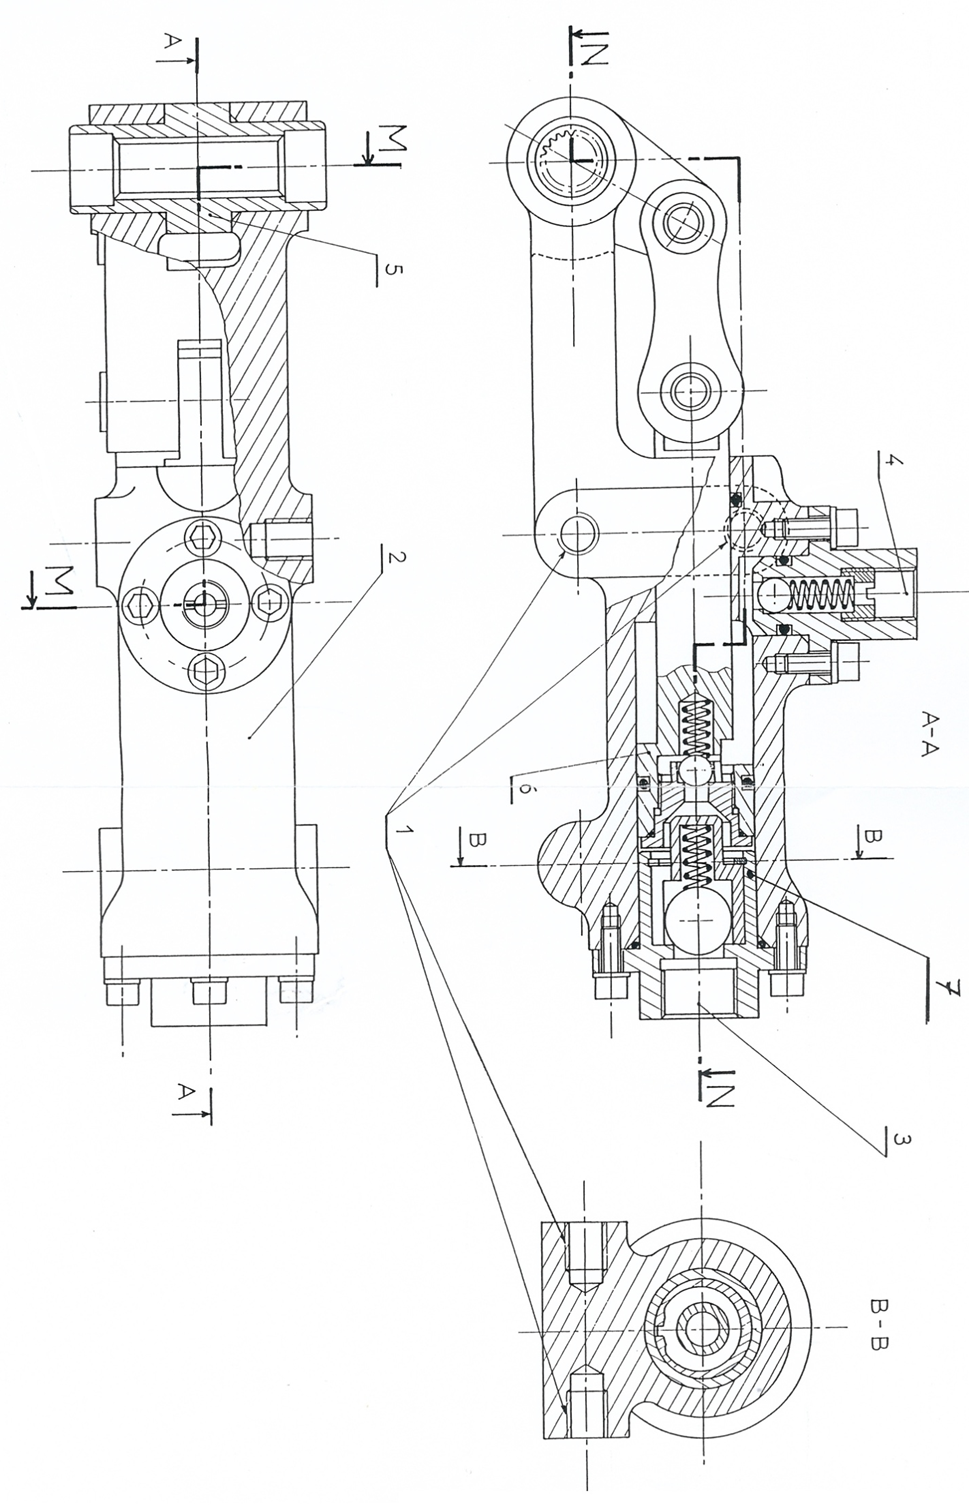
\includegraphics[width=.9\linewidth]{1020_02}
\end{marginfigure}
\fi


\ifprof
\else

\footnotesize
%\begin{marginfigure}
%\begin{tabular}{|p{.9\linewidth}|}
%\hline
%Indications (à vérifier...) :
%\begin{enumerate}
%\item $\vectv{B}{2}{0} = L\varphip(t)\vj{2} +\thetap(t)\left(L\vj{1}-R\vi{0}\right) $.
%\item  $\torseurcin{V}{2}{0} = \torseurl{\vecto{2}{0}=\left( \varphip(t)+\thetap(t) \right) \vk{0} }{ L\varphip(t)\vj{2} +\thetap(t)\left(L\vj{1}-R\vi{0}\right)}{B}$.
%\item $\vectg{B}{2}{0} =  L\varphipp(t)\vj{2}-L\varphip(t)\left(\varphip(t)+\thetap(t) \right)\vi{2}  + \thetapp(t)\left(L\vj{1}-R\vi{0}\right) - L\thetap^2(t)\vi{1}$.
%\end{enumerate} \\ \hline
%\end{tabular}
%\end{marginfigure}
\normalsize



\marginnote{Corrigé  voir \ref{CIN:01:B2:12:1020}.}

\fi 
 
\graphicspath{{\repStyle/png/}{../CIN/CIN-01-ModeliserSchemasCinematiques/10_PompePalette/images/}} 
\normalfalse \difficiletrue \tdifficilefalse
\correctiontrue

%\UPSTIidClasse{11} % 11 sup, 12 spé
%\newcommand{\UPSTIidClasse}{12}

\exer{Pompe à palettes  $\star\star$ \label{CIN:01:B2:12:10}}
\setcounter{question}{0}\marginnote{\xpComp{CIN}{01}}%\UPSTIcompetence{B2-12}
\index{Compétence B2-12}\index{Compétence CIN-01}
\index{Pompe à palettes}
\ifcorrection
\else
\marginnote{\textbf{Pas de corrigé pour cet exercice.}}
\fi

\ifprof
\else
Soit le mécanisme suivant. On a $\vect{AO}=e\vect{i_0}$ et $\vect{AB}=\lambda(t)\vect{i_1}$. De plus $e=\SI{10}{mm}$ et $R=\SI{20}{mm}$. Le contact entre \textbf{0} et \textbf{2} en $B$ est maintenu en permanence (notamment par effet centrifuge lors de la rotation de la pompe).
\begin{marginfigure}
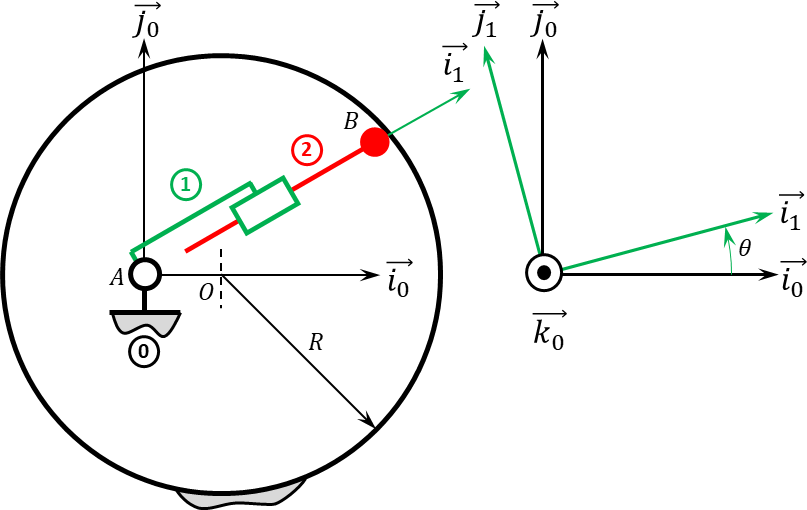
\includegraphics[width=\linewidth]{10_01}
\end{marginfigure}
\fi


\question{Tracer le graphe des liaisons.}
\ifprof
\begin{marginfigure}
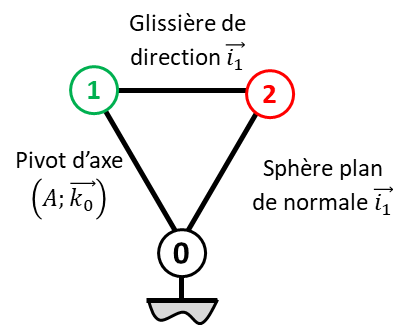
\includegraphics[width=5cm]{10_01_cor}
\end{marginfigure}
\else
\fi


\question{Retracer le schéma cinématique pour $\theta(t)=0 \,\text{rad}$.}
\ifprof
\begin{marginfigure}
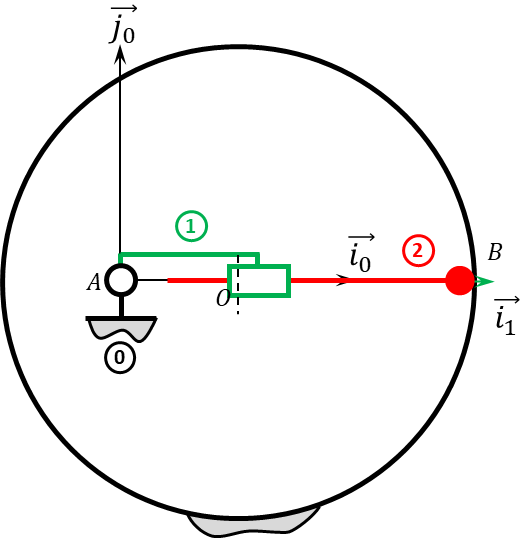
\includegraphics[width=5cm]{10_02_cor}
\end{marginfigure}
\else
\fi

\question{Retracer le schéma cinématique pour $\theta(t)=\pi\,\text{rad}$.}
\ifprof
\begin{marginfigure}
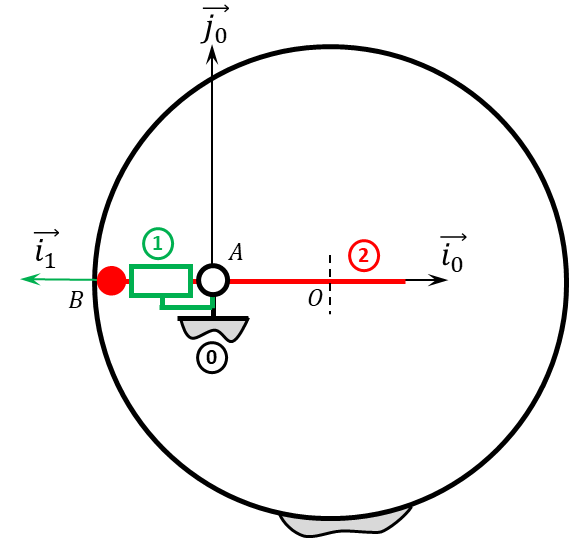
\includegraphics[width=5cm]{10_03_cor}
\end{marginfigure}

\else
\fi


\question{En déduire la course de la pièce \textbf{2}.}
\ifprof
La course de la pièce 2 est donnée par la différence entre la longueur $AB$ maximale et $AB$ minimale : $c= 30-10 = \SI{20}{mm}$.
\else
\fi



\ifprof
\else

\marginnote{Corrigé  voir \ref{CIN:01:B2:12:10}.}

\fi 
 
\graphicspath{{\repStyle/png/}{../CIN/CIN-01-ModeliserSchemasCinematiques/11_PompePistonsRadiaux/images/}} 
\normalfalse \difficiletrue \tdifficilefalse
\correctiontrue

%\UPSTIidClasse{11} % 11 sup, 12 spé
%\newcommand{\UPSTIidClasse}{12}

\exer{Pompe à pistons radiaux  $\star\star$ \label{CIN:01:B2:12:11}}
\setcounter{question}{0}\marginnote{\xpComp{CIN}{01}}%\UPSTIcompetence{B2-12}
\index{Compétence B2-12}\index{Compétence CIN-01}
\index{Pompe à pistons radiaux}
\index{Arbre à cames}
\ifcorrection
\else
\marginnote{\textbf{Pas de corrigé pour cet exercice.}}
\fi

\ifprof
\else
Soit le mécanisme suivant. On a $\vect{AB}=e\vect{i_1}$ et $\vect{BI}=R\vect{j_0}$. De plus, 
$e=\SI{10}{mm}$ et $R=\SI{20}{mm}$. Le contact entre \textbf{1} et \textbf{2} en $B$ est maintenu en permanence par un ressort suffisamment raide (non représenté) positionné entre \textbf{0} et \textbf{2}. 
\begin{marginfigure}
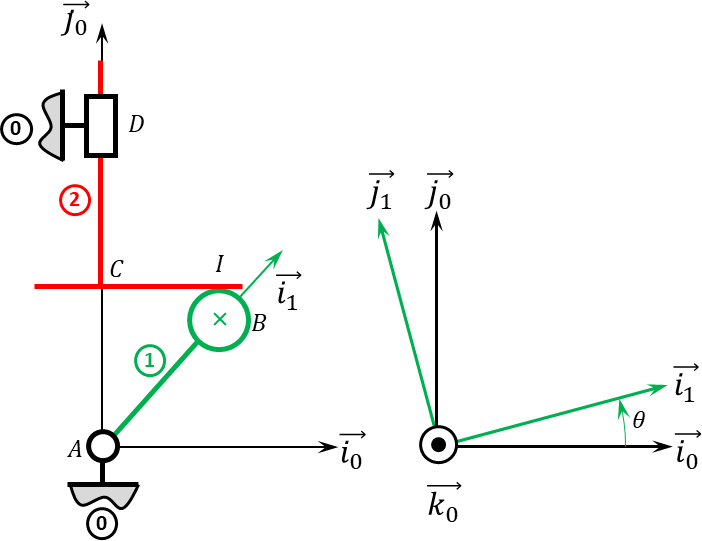
\includegraphics[width=\linewidth]{11_01}
\end{marginfigure}
\fi

\question{Tracer le graphe des liaisons.}
\ifprof
\begin{marginfigure}
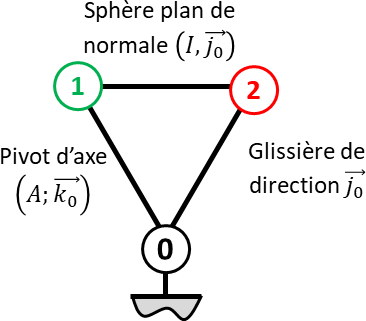
\includegraphics[width=4cm]{11_01_cor}
\end{marginfigure}
\else
\fi

\question{Retracer le schéma cinématique pour $\theta(t)=0 \,\text{rad}$.}
\ifprof
\else
\fi

\question{Retracer le schéma cinématique pour $\theta(t)=\dfrac{\pi}{2}\,\text{rad}$.}
\ifprof
\else
\fi

\question{Retracer le schéma cinématique pour $\theta(t)=-\dfrac{\pi}{2}\,\text{rad}$.}
\ifprof
\begin{marginfigure}
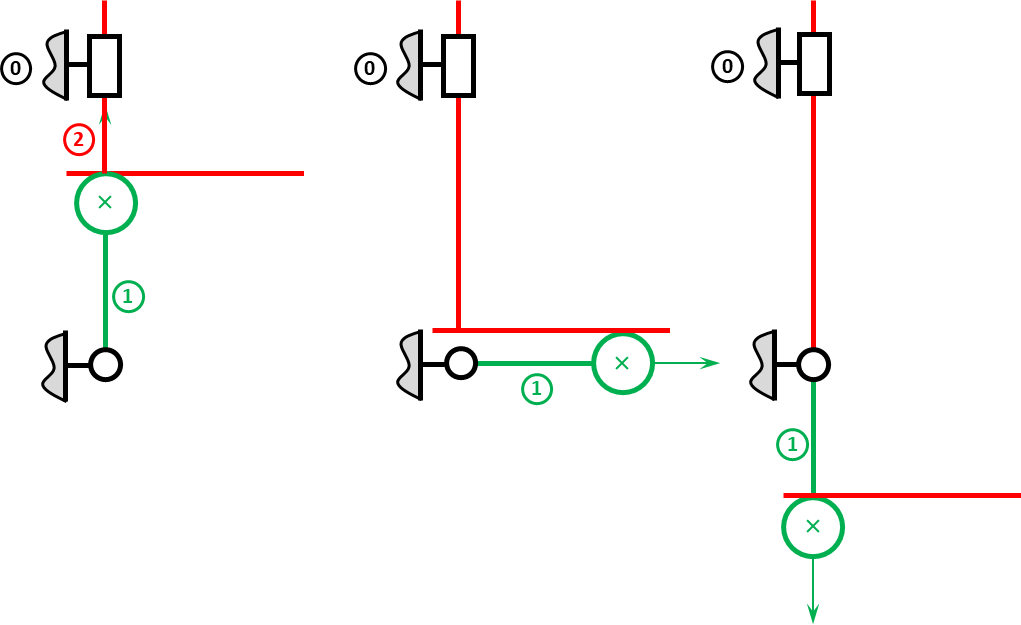
\includegraphics[width=8cm]{11_02_cor}
\end{marginfigure}
\else
\fi


\question{En déduire la course de la pièce \textbf{2}.}
\ifprof
La course est de 
\else
\fi



\ifprof
\else

\marginnote{Corrigé  voir \ref{CIN:01:B2:12:11}.}

\fi 
 
\graphicspath{{\repStyle/png/}{../CIN/CIN-01-ModeliserSchemasCinematiques/12_BielleManivelle/images/}} 
\normalfalse \difficiletrue \tdifficilefalse
\correctionfalse

%\UPSTIidClasse{11} % 11 sup, 12 spé
%\newcommand{\UPSTIidClasse}{12}

\exer{Système bielle manivelle  $\star\star$ \label{CIN:01:B2:12:12}}
\setcounter{question}{0}\marginnote{\xpComp{CIN}{01}}%\UPSTIcompetence{B2-12}
\index{Compétence B2-12}\index{Compétence CIN-01}
\index{Bielle Manivelle}
\index{Moteur}
\ifcorrection
\else
\marginnote{\textbf{Pas de corrigé pour cet exercice.}}
\fi

\ifprof
\else
Soit le mécanisme suivant. On a $\vect{AB}=R\vect{i_1}$ et $\vect{CB}=L\vect{i_2}$. De plus, 
$R=\SI{10}{mm}$ et $L=\SI{20}{mm}$. 

\begin{marginfigure}
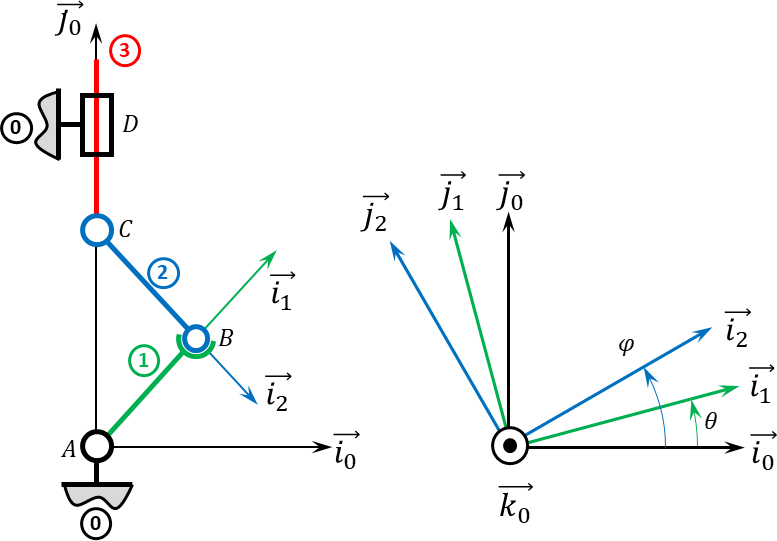
\includegraphics[width=\linewidth]{12_01}
\end{marginfigure}
\fi

\question{Tracer le graphe des liaisons.}
\ifprof
\else
\fi

\question{Retracer le schéma cinématique pour $\theta(t)=\dfrac{\pi}{2}\,\text{rad}$.}
\ifprof
\else
\fi

\question{Retracer le schéma cinématique pour $\theta(t)=-\dfrac{\pi}{2}\,\text{rad}$.}
\ifprof
\else
\fi


\question{En déduire la course de la pièce \textbf{3}.}
\ifprof
\else
\fi



\ifprof
\else
\marginnote{Corrigé  voir \ref{CIN:01:B2:12:12}.}
\fi 
 
\graphicspath{{\repStyle/png/}{../CIN/CIN-01-ModeliserSchemasCinematiques/13_TransfoMouvement/images/}} 
\normalfalse \difficilefalse \tdifficiletrue
\correctionfalse

%\UPSTIidClasse{11} % 11 sup, 12 spé
%\newcommand{\UPSTIidClasse}{12}

\exer{Système de transformation de mouvement  $\star\star$ \label{CIN:01:B2:12:13}}
\setcounter{question}{0}\marginnote{\xpComp{CIN}{01}}%\UPSTIcompetence{B2-12}
\index{Compétence B2-12}\index{Compétence CIN-01}
\index{Bielle Manivelle}
\index{Moteur}
\ifcorrection
\else
\marginnote{\textbf{Pas de corrigé pour cet exercice.}}
\fi

\ifprof
\else
Soit le mécanisme suivant. On a $\vect{AB}=R\vect{i_1}$ et $\vect{CA}=H\vect{j_0}$. De plus, 
$R=\SI{30}{mm}$ et $H=\SI{40}{mm}$. 

\begin{marginfigure}
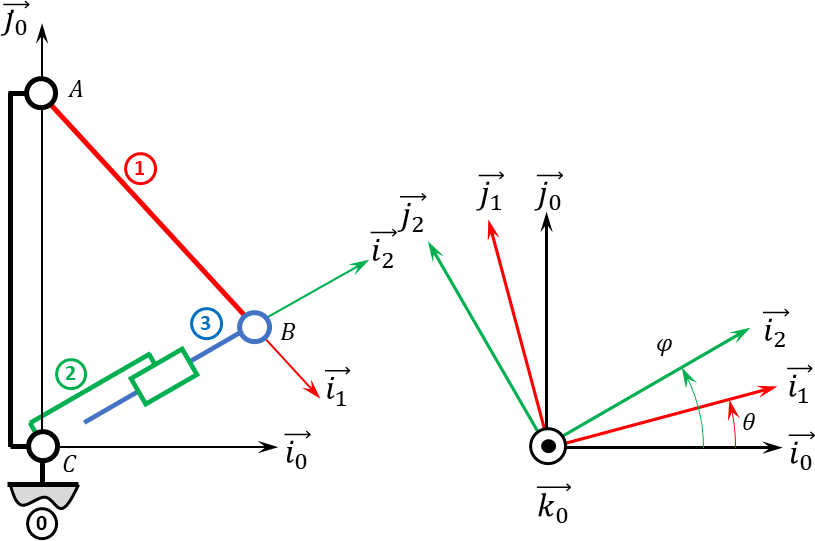
\includegraphics[width=\linewidth]{13_01}
\end{marginfigure}
\fi


\question{Tracer le graphe des liaisons.}
\ifprof
\else
\fi

\question{Retracer le schéma cinématique pour $\theta(t)=\dfrac{\pi}{2}\,\text{rad}$.}
\ifprof
\else
\fi

\question{Retracer le schéma cinématique pour $\theta(t)=0\,\text{rad}$.}
\ifprof
\else
\fi

\question{Retracer le schéma cinématique pour $\theta(t)=-\dfrac{\pi}{2}\,\text{rad}$.}
\ifprof
\else
\fi


\question{En déduire la course de la pièce \textbf{3}.}
\ifprof
\else
\fi



\ifprof
\else

\marginnote{Corrigé  voir \ref{CIN:01:B2:12:13}.}

\fi 
 
\graphicspath{{\repStyle/png/}{../CIN/CIN-01-ModeliserSchemasCinematiques/14_Sympact/images/}} 
\normalfalse \difficiletrue \tdifficilefalse
\correctiontrue

%\UPSTIidClasse{11} % 11 sup, 12 spé
%\newcommand{\UPSTIidClasse}{12}

\exer{Barrière Sympact $\star\star$ \label{CIN:01:B2:12:14}}
\setcounter{question}{0}\marginnote{\xpComp{CIN}{01}}%\UPSTIcompetence{B2-12}
\index{Compétence B2-12}\index{Compétence CIN-01}
\index{Barrière Sympact}
\ifcorrection
\else
\marginnote{\textbf{Pas de corrigé pour cet exercice.}}
\fi

\ifprof
\else
Soit le mécanisme suivant. On a $\vect{AC}=H\vect{j_0}$ et $\vect{CB}=R\vect{i_1}$. De plus, 
$H=\SI{120}{mm}$ et $R=\SI{40}{mm}$. 

\begin{marginfigure}
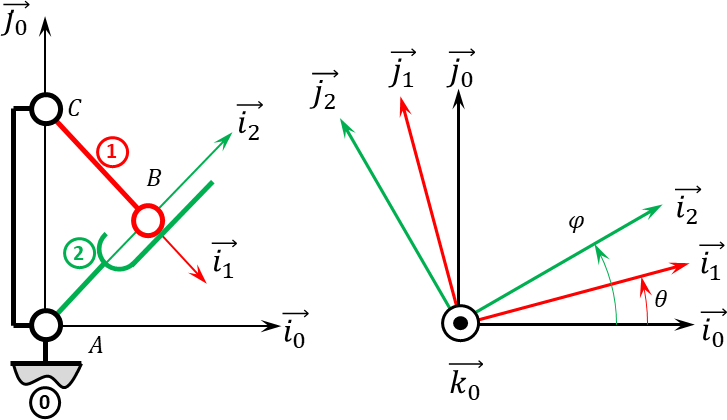
\includegraphics[width=\linewidth]{14_01}
\end{marginfigure}
\fi


\question{Tracer le graphe des liaisons.}
\ifprof
\begin{marginfigure}
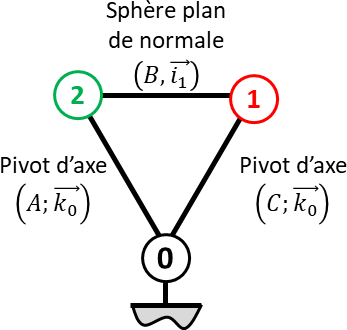
\includegraphics[width=.4\linewidth]{14_02_c}
\end{marginfigure}
\else
\fi

\question{Retracer le schéma cinématique pour $\theta(t)=\dfrac{\pi}{2}\,\text{rad}$.}
\ifprof
\begin{marginfigure}
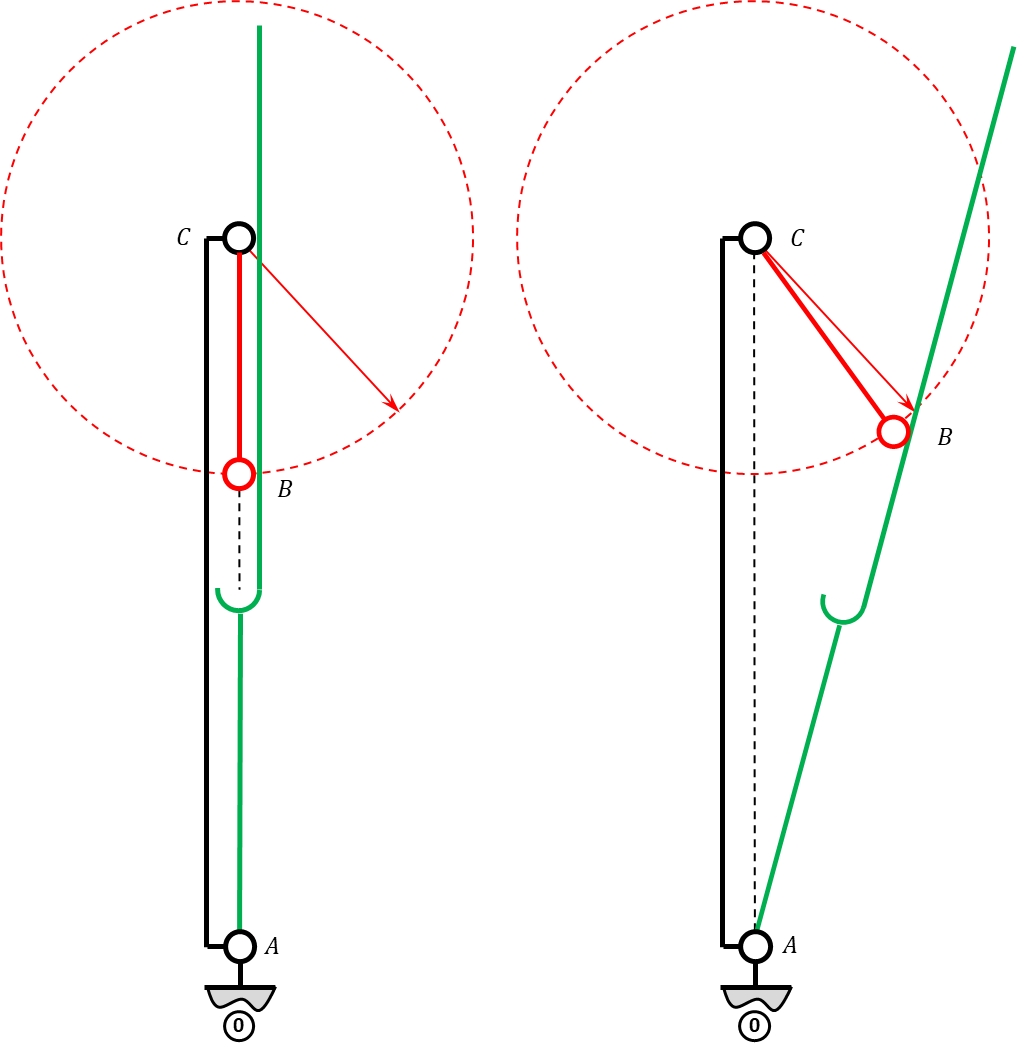
\includegraphics[width=.5\linewidth]{14_01_c}
\end{marginfigure}

\else
\fi

\question{Retracer le schéma cinématique pour $\theta(t)=75\degres$.}
\ifprof
\else
\fi


\question{Dans l'hypothèse où la pièce \textbf{1} peut faire des tours complets, quelle doit être la longueur minimale de la pièce \textbf{2}.}
\ifprof
Dans cas, dans le pire des cas, $A$, $B$ et $C$ sont alignés (avec $B$ au-dessus de $C$). Il faut donc $AB = AC+CB = \SI{160}{mm}$.
\else
\fi

\question{Dans l'hypothèse où la pièce \textbf{2} fait \SI{12}{cm}, quel sera le débattement maximal de la pièce \textbf{1}.}
\ifprof
Comme je suis paresseux, j'ai réalisé la construction avec geogebra. On mesure \SI{160,8}{\degres}.
\begin{marginfigure}
\rotatebox{90}{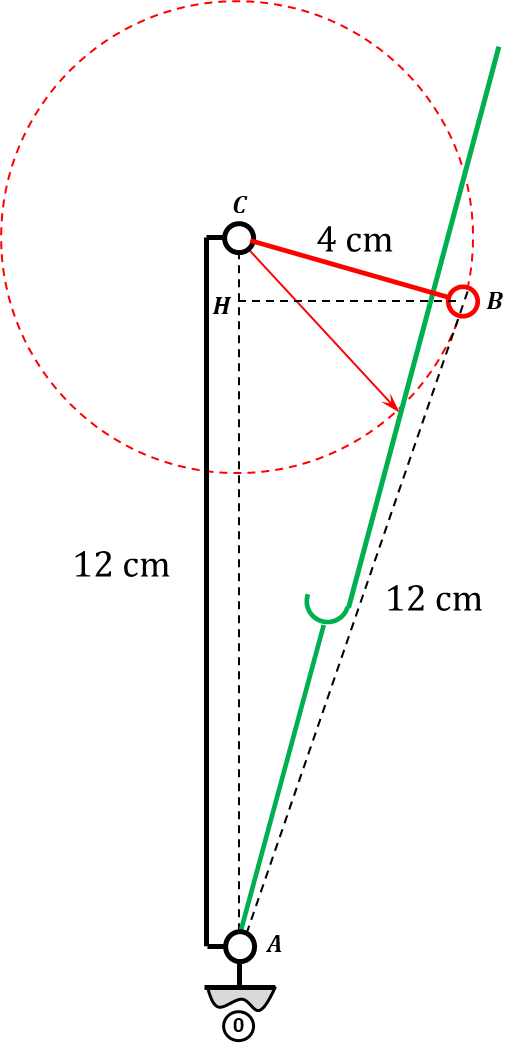
\includegraphics[width=.35\linewidth]{14_03_c}}
\end{marginfigure}
\else
\fi

\ifprof
\else
\ifcolle
\else
\marginnote{
\begin{solution}
\begin{enumerate}
\item .
\item .
\item .
\item \SI{160}{mm}.
\item \SI{160,8}{\degres}.
\end{enumerate}
\end{solution}
\fi
Corrigé  voir \ref{CIN:01:B2:12:14}.}
\fi 
 
\graphicspath{{\repStyle/png/}{../CIN/CIN-01-ModeliserSchemasCinematiques/15_SympactGalet/images/}} 
\normalfalse \difficiletrue \tdifficilefalse
\correctionfalse

%\UPSTIidClasse{11} % 11 sup, 12 spé
%\newcommand{\UPSTIidClasse}{12}

\exer{Barrière Sympact $\star\star$ \label{CIN:01:B2:12:15}}
\setcounter{question}{0}\marginnote{\xpComp{CIN}{01}}%\UPSTIcompetence{B2-12}
\index{Compétence B2-12}\index{Compétence CIN-01}
\index{Barrière Sympact}
\ifcorrection
\else
\marginnote{\textbf{Pas de corrigé pour cet exercice.}}
\fi
\ifprof
\else
Soit le mécanisme suivant. On a $\vect{AC}=H\vect{j_0}$ et $\vect{CB}=R\vect{i_1}$. De plus, 
$H=\SI{120}{mm}$, $R=\SI{40}{mm}$ $BI=\SI{10}{mm}$.

\begin{marginfigure}
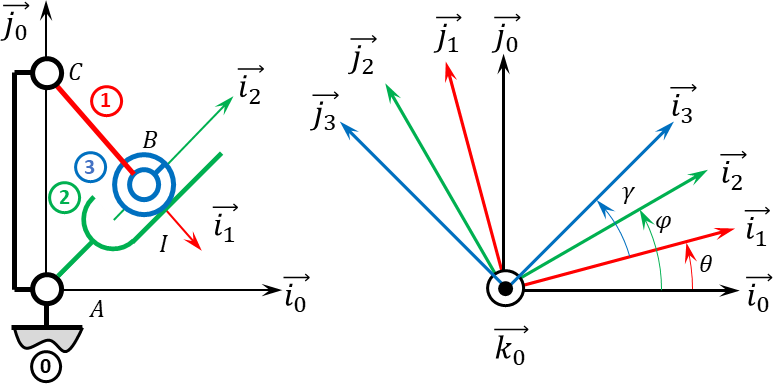
\includegraphics[width=\linewidth]{15_01}
\end{marginfigure}
\fi

\question{Tracer le graphe des liaisons.}
\ifprof
\else
\fi

\question{Retracer le schéma cinématique pour $\theta(t)=\dfrac{\pi}{2}\,\text{rad}$.}
\ifprof
\else
\fi

\question{Retracer le schéma cinématique pour $\theta(t)=-\dfrac{\pi}{2}\,\text{rad}$.}
\ifprof
\else
\fi


%\question{En déduire la course de la pièce \textbf{3}.}
%\ifprof
%\else
%\fi



\ifprof
\else
\marginnote{Corrigé voir \ref{CIN:01:B2:12:15}.}
\fi 
 
\graphicspath{{\repStyle/png/}{../CIN/CIN-01-ModeliserSchemasCinematiques/16_Poussoir/images/}} 
\normalfalse \difficiletrue \tdifficilefalse
\correctionfalse

%\UPSTIidClasse{11} % 11 sup, 12 spé
%\newcommand{\UPSTIidClasse}{12}

\exer{Poussoir $\star\star$ \label{CIN:01:B2:12:16}}
\setcounter{question}{0}\marginnote{\xpComp{CIN}{01}}%\UPSTIcompetence{B2-12}
\index{Compétence B2-12}\index{Compétence CIN-01}
%\index{Barrière Sympact}
\ifcorrection
\else
\marginnote{\textbf{Pas de corrigé pour cet exercice.}}
\fi

\ifprof
\else
Soit le mécanisme suivant. On a $\vect{AC}=L\vect{i_0}+H\vect{j_0}$. De plus, 
$H=\SI{120}{mm}$, $L=\SI{40}{mm}$.

\begin{marginfigure}
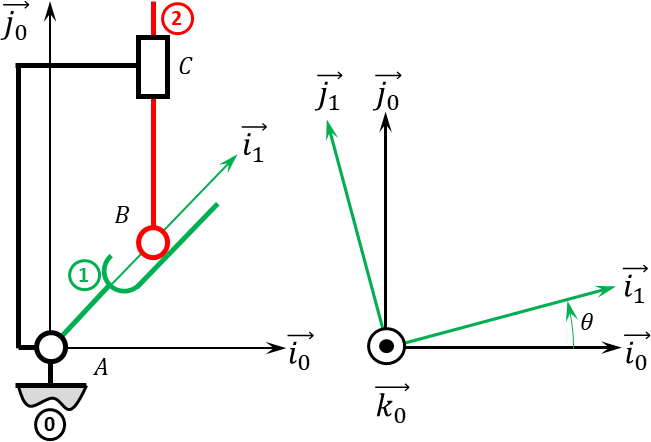
\includegraphics[width=\linewidth]{16_01}
\end{marginfigure}
\fi


\question{Tracer le graphe des liaisons.}
\ifprof
\else
\fi


\question{Retracer le schéma cinématique pour $\theta(t)=\dfrac{\pi}{4}\,\text{rad}$.}
\ifprof
\else
\fi

\question{Retracer le schéma cinématique pour $\theta(t)=-\dfrac{\pi}{4}\,\text{rad}$.}
\ifprof
\else
\fi


%\question{En déduire la course de la pièce \textbf{3}.}
%\ifprof
%\else
%\fi



\ifprof
\else

\marginnote{Corrigé  voir \ref{CIN:01:B2:12:16}.}

\fi 
 
\graphicspath{{\repStyle/png/}{../CIN/CIN-01-ModeliserSchemasCinematiques/17_4Barres/images/}} 
\normalfalse \difficilefalse \tdifficiletrue
\correctionfalse

%\UPSTIidClasse{11} % 11 sup, 12 spé
%\newcommand{\UPSTIidClasse}{12}

\exer{Système 4 barres $\star\star\star$ \label{CIN:01:B2:12:17}} 
\setcounter{question}{0}\marginnote{\xpComp{CIN}{01}}%\UPSTIcompetence{B2-12}
\index{Compétence B2-12}\index{Compétence CIN-01}
\index{Système 4 barres}
\ifcorrection
\else
\marginnote{\textbf{Pas de corrigé pour cet exercice.}}
\fi

\ifprof
\else
On a : 
%\begin{multicols}{2}
\begin{itemize}
\item $\vect{OA} = a \vx{1}-f \vy{1}$ avec $a=\SI{355}{mm}$ et $f=\SI{13}{mm}$;
\item $\vect{AB} = b \vx{2}$ avec $b=\SI{280}{mm}$;
\item $\vect{BC} = -c \vx{3}$ avec $c=\SI{280}{mm}$;
\item $\vect{OC} = -d \vx{0}-e\vy{0}$ avec $d=\SI{89,5}{mm}$ et $e=\SI{160}{mm}$;
\end{itemize}
%\end{multicols}
%a,b,c,d,e,ff = 355,280,280,89.5,160,13

\begin{marginfigure}
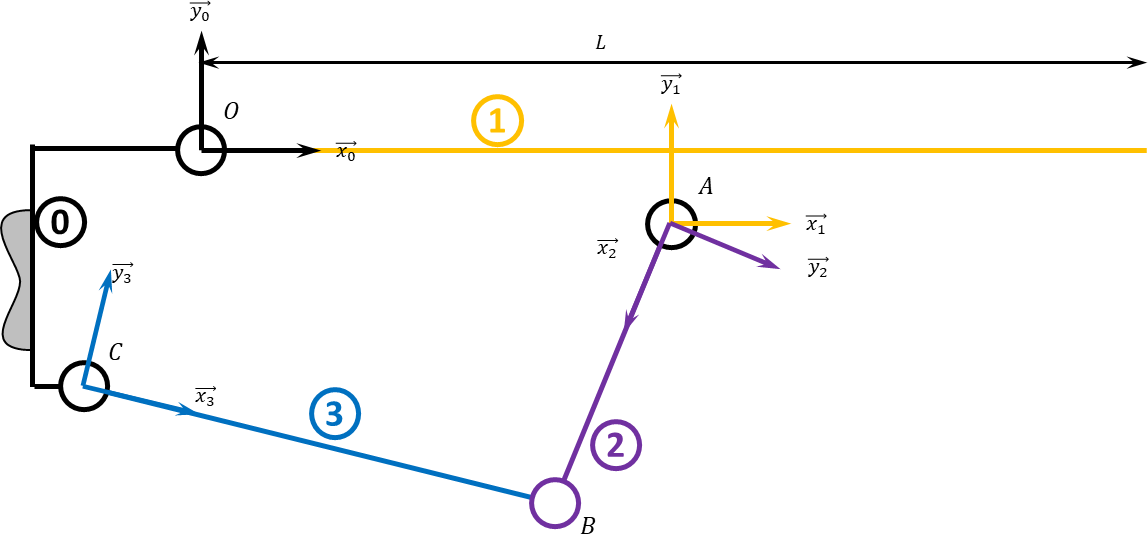
\includegraphics[width=\linewidth]{17_01}

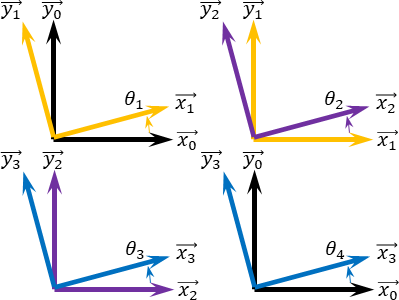
\includegraphics[width=\linewidth]{17_02}
\end{marginfigure}
\fi

\question{Tracer le graphe des liaisons.}
\ifprof
\else
\fi

\question{Retracer le schéma cinématique pour $\theta_1(t)=0\,\text{rad}$.}
\ifprof
\else
\fi

\question{Retracer le schéma cinématique pour $\theta_1(t)=-\dfrac{\pi}{2}\,\text{rad}$.}
\ifprof
\else
\fi


\question{En déduire la course angulaire ($\theta_4$) de la pièce \textbf{3}.}
\ifprof
\else
\fi



\ifprof
\else

\marginnote{Corrigé  voir \ref{CIN:01:B2:12:17}.}

\fi 
 
\graphicspath{{\repStyle/png/}{../CIN/CIN-01-ModeliserSchemasCinematiques/18_Maxpid/images/}} 
\normalfalse \difficilefalse \tdifficiletrue
\correctionfalse

%\UPSTIidClasse{11} % 11 sup, 12 spé
%\newcommand{\UPSTIidClasse}{12}

\exer{Maxpid $\star\star\star$ \label{CIN:01:B2:12:18}}
\setcounter{question}{0}\marginnote{\xpComp{CIN}{01}}%\UPSTIcompetence{B2-12}
\index{Compétence B2-12}\index{Compétence CIN-01}
\index{Maxpid}
\ifcorrection
\else
\marginnote{\textbf{Pas de corrigé pour cet exercice.}}
\fi

\ifprof
\else

Soit le schéma suivant. 
\begin{marginfigure}
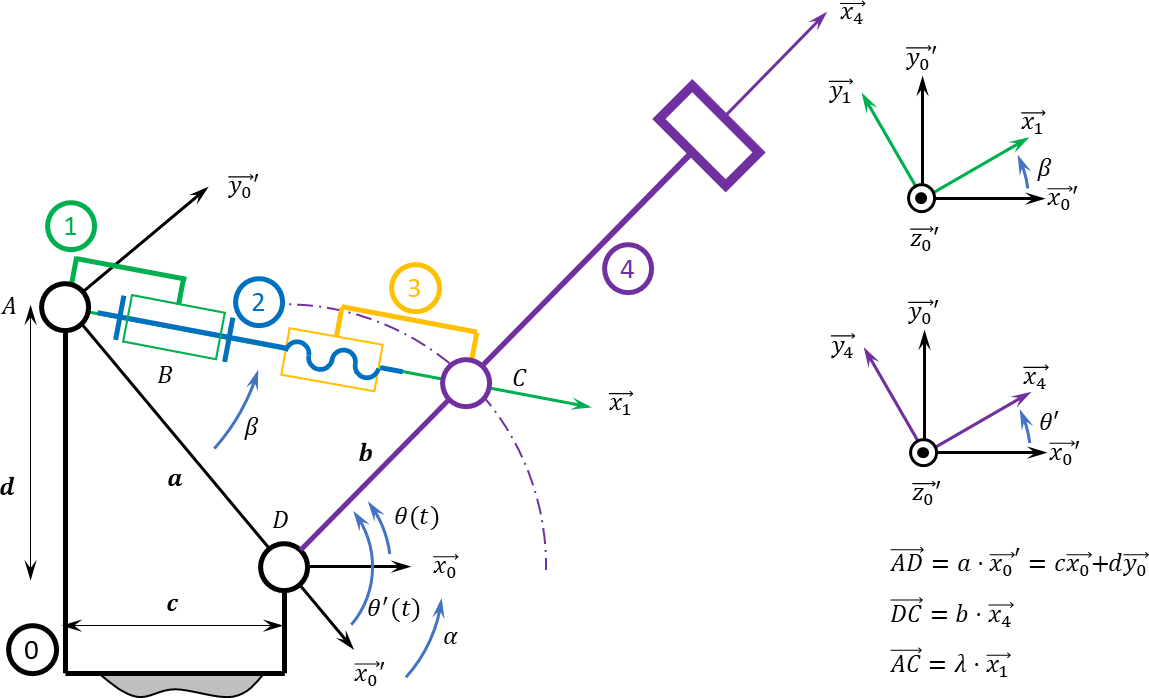
\includegraphics[width=\linewidth]{18_01}
\end{marginfigure}
\fi

Par ailleurs $a=\SI{107,1}{mm}$, $b=\SI{80}{mm}$, $c=\SI{70}{mm}$, $d=\SI{80}{mm}$. Le pas de la vis est de $\SI{4}{mm}$.


\question{Tracer le graphe des liaisons.}
\ifprof
\else
\fi

\question{Retracer le schéma cinématique pour $\theta(t)=0\,\text{rad}$.}
\ifprof
\else
\fi

\question{Retracer le schéma cinématique pour $\theta(t)=\dfrac{\pi}{2}\,\text{rad}$.}
\ifprof
\else
\fi


\question{En déduire la course de $\lambda$.}
\ifprof
\else
\fi



\ifprof
\else

\marginnote{Corrigé  voir \ref{CIN:01:B2:12:18}.}

\fi 
 
\graphicspath{{\repStyle/png/}{../CIN/CIN-01-ModeliserSchemasCinematiques/46_RR_RSG/images/}} 
\normalfalse \difficiletrue \tdifficilefalse
\correctionfalse

%\UPSTIidClasse{11} % 11 sup, 12 spé
%\newcommand{\UPSTIidClasse}{12}

\exer{Mouvement RR -- RSG  $\star\star$ \label{CIN:01:B2:12:46}}
\setcounter{question}{0}\marginnote{\xpComp{CIN}{01}}%\UPSTIcompetence{B2-12}
\index{Compétence B2-12}\index{Compétence CIN-01}
\index{Mécanisme à 1 rotations, 1 translation et RSG}
\ifcorrection
\else
\marginnote{\textbf{Pas de corrigé pour cet exercice.}}
\fi

\ifprof
\else
Soit le mécanisme suivant. On a $\vect{IA}=R\vect{j_0}$ et $\vect{AB}=L\vect{i_1}$. De plus $R=\SI{15}{mm}$.
\begin{marginfigure}
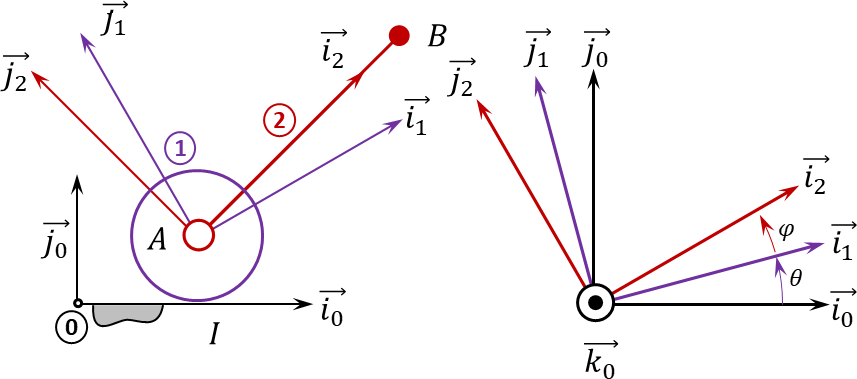
\includegraphics[width=\linewidth]{46_RR_RSG_01}
\end{marginfigure}
\fi


\question{Tracer le graphe des liaisons.}
\ifprof
\else
\fi


\question{Retracer le schéma cinématique pour $\theta(t)=0\,\text{rad}$ et $\varphi(t)=0\,\text{rad}$. On notera $I_0$ le point de contact entre \textbf{0} et \textbf{1}.}
\ifprof
\else
\fi

\question{Retracer le schéma cinématique pour $\theta(t)=\dfrac{\pi}{2}\,\text{rad}$ et $\varphi(t)=0\,\text{rad}$. On notera $I_1$ le point de contact entre \textbf{0} et \textbf{1}. On précisera la position des points $I_{0,0}$ et $I_{0,1}$, points résultants de la rupture de contact lors du passage de $\theta(t)$ de 0 à $\dfrac{\pi}{2}$.}
\ifprof
\else
\fi


\question{Retracer le schéma cinématique pour $\theta(t)=\dfrac{\pi}{2}\,\text{rad}$ et $\varphi(t)=\dfrac{\pi}{2}\,\text{rad}$.} 
\ifprof
\else
\fi


\ifprof
\else

\marginnote{Corrigé  voir \ref{CIN:01:B2:12:46}.}

\fi 
 
\graphicspath{{\repStyle/png/}{../CIN/CIN-01-ModeliserSchemasCinematiques/513_Divers_Tabouret/images/}} 
\normalfalse \difficiletrue \tdifficilefalse
\correctionfalse

%\UPSTIidClasse{11} % 11 sup, 12 spé
%\newcommand{\UPSTIidClasse}{12}

\exer{Tabouret  $\star\star$ \label{CIN:01:B2:12:513}}
\setcounter{question}{0}\marginnote{\xpComp{CIN}{01}}%\UPSTIcompetence{B2-12}
\index{Compétence B2-12}\index{Compétence CIN-01}

\ifcorrection
\else
\marginnote{\textbf{Pas de corrigé pour cet exercice.}}
\fi

\ifprof
\else
\begin{marginfigure}
\centering
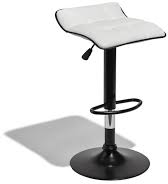
\includegraphics[width=.5\linewidth]{513_01}
\end{marginfigure}
\fi


\question{Proposer un schéma cinématique permettant de modéliser la liaison entre l'assise et le sol.}
\ifprof
\else
\fi

\ifprof
\else

\marginnote{Corrigé  voir \ref{CIN:01:B2:12:513}.}

\fi 
 
\graphicspath{{\repStyle/png/}{../CIN/CIN-01-ModeliserSchemasCinematiques/514_Divers_Tabouret/images/}} 
\normalfalse \difficiletrue \tdifficilefalse
\correctionfalse

%\UPSTIidClasse{11} % 11 sup, 12 spé
%\newcommand{\UPSTIidClasse}{12}

\exer{Tabouret  $\star\star$ \label{CIN:01:B2:12:514}}
\setcounter{question}{0}\marginnote{\xpComp{CIN}{01}}%\UPSTIcompetence{B2-12}
\index{Compétence B2-12}\index{Compétence CIN-01}

\ifcorrection
\else
\marginnote{\textbf{Pas de corrigé pour cet exercice.}}
\fi

\ifprof
\else
\begin{marginfigure}
\centering
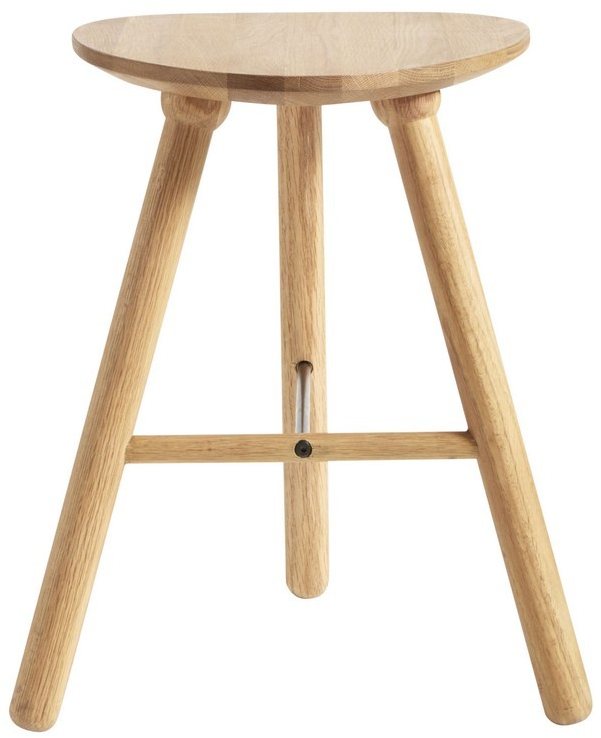
\includegraphics[width=.3\linewidth]{514_01}
\end{marginfigure}
\fi


\question{Proposer 3 schémas cinématiques permettant de modéliser les contacts entre le sol et le tabouret.}
\ifprof
\else
\fi

\ifprof
\else

\marginnote{Corrigé  voir \ref{CIN:01:B2:12:514}.}

\fi 
 
\graphicspath{{\repStyle/png/}{../CIN/CIN-01-Parametrage/01_T/images/}} 
\normaltrue
\correctiontrue

%\UPSTIidClasse{11} % 11 sup, 12 spé
%\newcommand{\UPSTIidClasse}{12}

\exer{Mouvement T -- $\star$ \label{CIN:01:B2:13:PTSI:01}}
\setcounter{question}{0}\marginnote{\xpComp{CIN}{01}}%\UPSTIcompetence[2]{B2-13}
\index{Compétence C2-05}\index{Compétence CIN-01}
\index{Compétence B2-13-PTSI}
\index{Mécanisme à 1 translation}
\ifcorrection
\else
\marginnote{\textbf{Pas de corrigé pour cet exercice.}}
\fi

\ifprof
\else
Soit le mécanisme suivant. 
\begin{marginfigure}
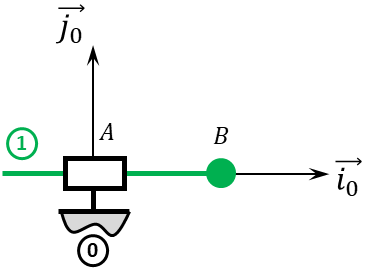
\includegraphics[width=\linewidth]{01_T_01}
\end{marginfigure}
\fi

\question{Réaliser le paramétrage du mécanisme.}
\ifprof~\\
Il n'y a ici que la distance $AB$ à paramétrer. On note $\vect{AB}=\lambda(t)\vi{0}$.
\else
\fi




\ifprof
\else


\marginnote{Corrigé voir \ref{CIN:01:B2:13:PTSI:01}.}

\fi


 
 
\graphicspath{{\repStyle/png/}{../CIN/CIN-01-Parametrage/01_T_02/images/}} 
\normaltrue
\correctionfalse

%\UPSTIidClasse{11} % 11 sup, 12 spé
%\newcommand{\UPSTIidClasse}{12}

\exer{Mouvement T -- $\star$ \label{CIN:01:B2:13:PTSI:01:02}}
\setcounter{question}{0}\marginnote{\xpComp{CIN}{01}}%\UPSTIcompetence[2]{B2-13}
\index{Compétence B2-13-PTSI}
\index{Mécanisme à 1 translation}
\ifcorrection
\else
\marginnote{\textbf{Pas de corrigé pour cet exercice.}}
\fi

\ifprof
\else ~\\
Soit le mécanisme suivant. On note $\vect{AB}=\lambda(t)\vect{i_0}$.
\begin{marginfigure}
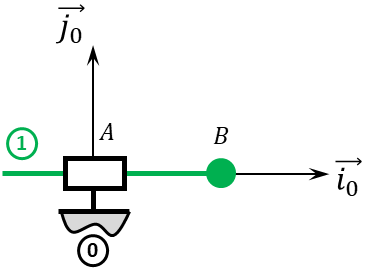
\includegraphics[width=\linewidth]{01_T_01}
\end{marginfigure}
\fi

\question{Réaliser le paramétrage du mécanisme.}
\ifprof ~\\

\else
\fi



\ifprof
\else
\footnotesize

\normalsize

\marginnote{Corrigé voir \ref{CIN:01:B2:13:PTSI:01:02}.}

\fi


 
 
\graphicspath{{\repStyle/png/}{../CIN/CIN-01-Parametrage/02_R/images/}} 
\normaltrue
\correctionfalse

%\UPSTIidClasse{11} % 11 sup, 12 spé
%\newcommand{\UPSTIidClasse}{12}

%\section{Rotation simple} %\label{B2:12:01}
\exer{Mouvement R  $\star$ \label{CIN:01:B2:13:PTSI:02}}
\setcounter{question}{0}\UPSTIcompetence[2]{C2-05}
\marginnote{\xpComp{CIN}{01}}%\UPSTIcompetence[2]{B2-13}
\index{Compétence C2-05}\index{Compétence CIN-01}
\index{Compétence B2-13-PTSI}
\index{Mécanisme à 1 rotation}
\ifcorrection
\else
\marginnote{\textbf{Pas de corrigé pour cet exercice.}}
\fi

\ifprof
\else
Soit le mécanisme suivant. On a $\vect{AB}=R\vect{i_1}$ avec $R=\SI{20}{mm}$. 
\begin{marginfigure}
\includegraphics[width=\linewidth]{02_R_01}
\end{marginfigure}
\fi

\question{Réaliser le paramétrage du mécanisme.}
\ifprof
\else
\fi


\ifprof
\else
\footnotesize

\normalsize

\marginnote{Corrigé voir \ref{CIN:01:B2:13:PTSI:02}.}

\fi 
 
\graphicspath{{\repStyle/png/}{../CIN/CIN-01-Parametrage/02_R_02/images/}} 
\normaltrue
\correctionfalse

%\UPSTIidClasse{11} % 11 sup, 12 spé
%\newcommand{\UPSTIidClasse}{12}

%\section{Rotation simple} %\label{B2:12:01}
\exer{Mouvement R  $\star$ \label{CIN:01:B2:13:PTSI:02}}
\setcounter{question}{0}
\marginnote{\xpComp{CIN}{01}}%\UPSTIcompetence[2]{B2-13}

\index{Compétence B2-13-PTSI}
\index{Mécanisme à 1 rotation}
\ifcorrection
\else
\marginnote{\textbf{Pas de corrigé pour cet exercice.}}
\fi

\ifprof
\else
Soit le mécanisme suivant. 
\begin{marginfigure}
\includegraphics[width=\linewidth]{02_R_01}
\end{marginfigure}
\fi

\question{Réaliser le paramétrage du mécanisme.}
\ifprof ~\\

\else
\fi


\ifprof
\else
\marginnote{Corrigé voir \ref{CIN:01:B2:13:PTSI:02}.}
\fi 
 
\graphicspath{{\repStyle/png/}{../CIN/CIN-01-Parametrage/03_TT/images/}} 
\normaltrue
\correctionfalse

%\UPSTIidClasse{11} % 11 sup, 12 spé
%\newcommand{\UPSTIidClasse}{12}


\exer{Mouvement TT -- $\star$ \label{CIN:01:B2:13:PTSI:03}}
\setcounter{question}{0}\UPSTIcompetence[2]{C2-05}
\marginnote{\xpComp{CIN}{01}}%\UPSTIcompetence[2]{B2-13}
\index{Compétence C2-05}\index{Compétence CIN-01}
\index{Compétence B2-13-PTSI}
\index{Mécanisme à 2 translations}
\ifcorrection
\else
\marginnote{\textbf{Pas de corrigé pour cet exercice.}}
\fi

\ifprof
\else
Soit le mécanisme suivant. 
\begin{marginfigure}
\includegraphics[width=\linewidth]{03_TT_01}
\end{marginfigure}
\fi

\question{Réaliser le paramétrage du mécanisme.}
\ifprof ~\\
\else
\fi




\ifprof
\else
\footnotesize

\normalsize

\marginnote{Corrigé voir \ref{CIN:01:B2:13:PTSI:03}.}

\fi


 
 
\graphicspath{{\repStyle/png/}{../CIN/CIN-01-Parametrage/03_TT_02/images/}} 
\normaltrue
\correctionfalse

%\UPSTIidClasse{11} % 11 sup, 12 spé
%\newcommand{\UPSTIidClasse}{12}


\exer{Mouvement TT -- $\star$ \label{CIN:01:B2:13:PTSI:03:02}}
\setcounter{question}{0}\UPSTIcompetence{B2-13}
\index{Compétence B2-13-PTSI}
\index{Mécanisme à 2 translations}
\ifcorrection
\else
\marginnote{\textbf{Pas de corrigé pour cet exercice.}}
\fi

\ifprof
\else
Soit le mécanisme suivant. 
\begin{marginfigure}
\includegraphics[width=\linewidth]{03_TT_01}
\end{marginfigure}
\fi

\question{Réaliser le paramétrage du mécanisme.}
\ifprof~\\ 

\else
\fi

\ifprof
\else
\footnotesize

\normalsize

\marginnote{Corrigé voir \ref{CIN:01:B2:13:PTSI:03:02}.}

\fi


 
 
\graphicspath{{\repStyle/png/}{../CIN/CIN-01-Parametrage/04_RR/images/}} 
\normaltrue
\correctionfalse

%\UPSTIidClasse{11} % 11 sup, 12 spé
%\newcommand{\UPSTIidClasse}{12}

\exer{Mouvement RR  $\star$ \label{CIN:01:B2:13:PTSI:04}}
\setcounter{question}{0}\UPSTIcompetence[2]{C2-05}
\marginnote{\xpComp{CIN}{01}}%\UPSTIcompetence[2]{B2-13}
\index{Compétence C2-05}\index{Compétence CIN-01}
\index{Compétence B2-13-PTSI}
\index{Mécanisme à 2 rotations}
\ifcorrection
\else
\marginnote{\textbf{Pas de corrigé pour cet exercice.}}
\fi

\ifprof
\else
Soit le mécanisme suivant. 
\begin{marginfigure}
\includegraphics[width=\linewidth]{04_RR_01}
\end{marginfigure}
\fi

\question{Réaliser le paramétrage du mécanisme.}
\ifprof~\\
\else
\fi



\ifprof
\else
\marginnote{Corrigé voir \ref{CIN:01:B2:13:PTSI:04}.}

\fi 
 
\graphicspath{{\repStyle/png/}{../CIN/CIN-01-Parametrage/04_RR_02/images/}} 
\normaltrue
\correctionfalse

%\UPSTIidClasse{11} % 11 sup, 12 spé
%\newcommand{\UPSTIidClasse}{12}

\exer{Mouvement RR  $\star$ \label{CIN:01:B2:13:PTSI:04:02}}
\setcounter{question}{0}\UPSTIcompetence{B2-13}
\index{Compétence B2-13-PTSI}
\index{Mécanisme à 2 rotations}
\ifcorrection
\else
\marginnote{\textbf{Pas de corrigé pour cet exercice.}}
\fi

\ifprof
\else
Soit le mécanisme suivant. 
\begin{marginfigure}
\includegraphics[width=\linewidth]{04_RR_01}
\end{marginfigure}
\fi

\question{Réaliser le paramétrage du mécanisme.}
\ifprof ~\\
\else

\fi



\ifprof
\else
\footnotesize

\normalsize
\marginnote{Corrigé voir \ref{CIN:01:B2:13:PTSI:04:02}.}

\fi 
 
\graphicspath{{\repStyle/png/}{../CIN/CIN-01-Parametrage/05_RT/images/}} 
\normaltrue
\correctionfalse

%\UPSTIidClasse{11} % 11 sup, 12 spé
%\newcommand{\UPSTIidClasse}{12}

\exer{Mouvement RT  $\star$ \label{CIN:01:B2:13:PTSI:05}}
\setcounter{question}{0}\UPSTIcompetence[2]{C2-05}
\marginnote{\xpComp{CIN}{01}\xpComp{GEO}{02}}%\UPSTIcompetence[2]{B2-13}
\index{Compétence C2-05}\index{Compétence CIN-01}
\index{Compétence B2-13-PTSI}
\index{Mécanisme à 1 rotation et 1 translation}
\ifcorrection
\else
\marginnote{\textbf{Pas de corrigé pour cet exercice.}}
\fi

\ifprof
\else
Soit le mécanisme suivant. 
\begin{marginfigure}
\includegraphics[width=\linewidth]{05_RT_01}
\end{marginfigure}
\fi

\question{Réaliser le paramétrage du mécanisme.}
\ifprof
\else
\fi


\ifprof
\else
\marginnote{Corrigé voir \ref{CIN:01:B2:13:PTSI:05}.}

\fi 
 
\graphicspath{{\repStyle/png/}{../CIN/CIN-01-Parametrage/05_RT_02/images/}} 
\normaltrue
\correctionfalse

%\UPSTIidClasse{11} % 11 sup, 12 spé
%\newcommand{\UPSTIidClasse}{12}

\exer{Mouvement RT  $\star$ \label{CIN:01:B2:13:PTSI:05:02}}
\setcounter{question}{0}\UPSTIcompetence{B2-13}
\index{Compétence B2-13-PTSI}
\index{Mécanisme à 1 rotation et 1 translation}
\ifcorrection
\else
\marginnote{\textbf{Pas de corrigé pour cet exercice.}}
\fi

\ifprof
\else
Soit le mécanisme suivant. On a $\vect{AB}=\lambda(t)\vect{i_1}$.
\begin{marginfigure}
\includegraphics[width=\linewidth]{05_RT_01}
\end{marginfigure}
\fi

\question{Réaliser le paramétrage du mécanisme.}
\ifprof  ~\\

\else
\fi



\ifprof
\else
\footnotesize

\normalsize

\marginnote{Corrigé voir \ref{CIN:01:B2:13:PTSI:05:02}.}

\fi 
 
\graphicspath{{\repStyle/png/}{../CIN/CIN-01-Parametrage/06_TR/images/}} 
\normaltrue
\correctionfalse

%\UPSTIidClasse{11} % 11 sup, 12 spé
%\newcommand{\UPSTIidClasse}{12}

\exer{Mouvement RT  $\star$ \label{CIN:01:B2:13:PTSI:06}}
\setcounter{question}{0}\UPSTIcompetence[2]{C2-05}
\marginnote{\xpComp{CIN}{01}}%\UPSTIcompetence[2]{B2-13}
\index{Compétence C2-05}\index{Compétence CIN-01}
\index{Compétence B2-13-PTSI}
\index{Mécanisme à 1 translation et 1 rotation}
\ifcorrection
\else
\marginnote{\textbf{Pas de corrigé pour cet exercice.}}
\fi

\ifprof
\else
Soit le mécanisme suivant. 
\begin{marginfigure}
\includegraphics[width=\linewidth]{06_TR_01}
\end{marginfigure}
\fi

\question{Réaliser le paramétrage du mécanisme.}
\ifprof
\else
\fi

\ifprof
\else
\marginnote{Corrigé voir \ref{CIN:01:B2:13:PTSI:06}.}

\fi 
 
\graphicspath{{\repStyle/png/}{../CIN/CIN-01-Parametrage/06_TR_02/images/}} 
\normaltrue
\correctionfalse

%\UPSTIidClasse{11} % 11 sup, 12 spé
%\newcommand{\UPSTIidClasse}{12}

\exer{Mouvement RT  $\star$ \label{CIN:01:B2:13:PTSI:06:02}}
\setcounter{question}{0}\UPSTIcompetence{B2-13}
\index{Compétence B2-13-PTSI}
\index{Mécanisme à 1 translation et 1 rotation}
\ifcorrection
\else
\marginnote{\textbf{Pas de corrigé pour cet exercice.}}
\fi

\ifprof
\else
Soit le mécanisme suivant. 
\begin{marginfigure}
\includegraphics[width=\linewidth]{06_TR_01}
\end{marginfigure}
\fi

\question{Réaliser le paramétrage du mécanisme.}
\ifprof ~\\

\else
\fi

\ifprof
\else
\footnotesize

\normalsize
\marginnote{Corrigé voir \ref{CIN:01:B2:13:PTSI:06:02}.}

\fi 
 
\graphicspath{{\repStyle/png/}{../CIN/CIN-01-Parametrage/07_RR3D/images/}} 
\normalfalse \difficiletrue \tdifficilefalse
\correctionfalse

%\UPSTIidClasse{11} % 11 sup, 12 spé
%\newcommand{\UPSTIidClasse}{12}

\exer{Mouvement RR 3D  $\star\star$ \label{CIN:01:B2:13:PTSI:07}}
\setcounter{question}{0}\UPSTIcompetence[2]{C2-05}
\marginnote{\xpComp{CIN}{01}}%\UPSTIcompetence[2]{B2-13}
\index{Compétence C2-05}\index{Compétence CIN-01}
\index{Compétence B2-13-PTSI}
\index{Mécanisme à 2 rotations 3D}
\ifcorrection
\else
\marginnote{\textbf{Pas de corrigé pour cet exercice.}}
\fi

\ifprof
\else
Soit le mécanisme suivant. 
\begin{marginfigure}
\includegraphics[width=\linewidth]{07_RR3D_01}
\end{marginfigure}
\fi

\question{Réaliser le paramétrage du mécanisme.}
\ifprof
\else
\fi



\ifprof
\else
\footnotesize

\normalsize

\marginnote{Corrigé voir \ref{CIN:01:B2:13:PTSI:07}.}

\fi 
 
\graphicspath{{\repStyle/png/}{../CIN/CIN-01-Parametrage/07_RR3D_02/images/}} 
\normaltrue \difficilefalse \tdifficilefalse
\correctionfalse

%\UPSTIidClasse{11} % 11 sup, 12 spé
%\newcommand{\UPSTIidClasse}{12}

\exer{Mouvement RR 3D  $\star$ \label{CIN:01:B2:13:PTSI:07:02}}
\setcounter{question}{0}\UPSTIcompetence{B2-13}
\index{Compétence B2-13-PTSI}
\index{Mécanisme à 2 rotations 3D}
\ifcorrection
\else
\marginnote{\textbf{Pas de corrigé pour cet exercice.}}
\fi

\ifprof
\else
Soit le mécanisme suivant. 
\begin{marginfigure}
\includegraphics[width=\linewidth]{07_RR3D_01}
\end{marginfigure}
\fi

\question{Réaliser le paramétrage du mécanisme.}
\ifprof ~\\

\else
\fi





\ifprof
\else
\footnotesize

\normalsize

\marginnote{Corrigé voir \ref{CIN:01:B2:13:PTSI:07}.}

\fi 
 
\graphicspath{{\repStyle/png/}{../CIN/CIN-01-Parametrage/08_RR3D/images/}} 
\normalfalse \difficiletrue \tdifficilefalse
\correctionfalse

%\UPSTIidClasse{11} % 11 sup, 12 spé
%\newcommand{\UPSTIidClasse}{12}

\exer{Mouvement RR 3D  $\star\star$ \label{CIN:01:B2:13:PTSI:08}}
\setcounter{question}{0}\UPSTIcompetence[2]{C2-05}
\marginnote{\xpComp{CIN}{01}}%\UPSTIcompetence[2]{B2-13}
\index{Compétence C2-05}\index{Compétence CIN-01}
\index{Compétence B2-13-PTSI}
\index{Mécanisme à 2 rotations 3D}
\ifcorrection
\else
\marginnote{\textbf{Pas de corrigé pour cet exercice.}}
\fi

\ifprof
\else
Soit le mécanisme suivant. 
\begin{marginfigure}
\includegraphics[width=\linewidth]{08_RR3D_01}
\end{marginfigure}
\fi

\question{Réaliser le paramétrage du mécanisme.}
\ifprof
\else
\fi



\ifprof
\else
\footnotesize

\normalsize
\marginnote{Corrigé voir \ref{CIN:01:B2:13:PTSI:08}.}

\fi 
 
\graphicspath{{\repStyle/png/}{../CIN/CIN-01-Parametrage/08_RR3D_02/images/}} 
\normalfalse \difficiletrue \tdifficilefalse
\correctionfalse

%\UPSTIidClasse{11} % 11 sup, 12 spé
%\newcommand{\UPSTIidClasse}{12}

\exer{Mouvement RR 3D  $\star$ \label{CIN:01:B2:13:PTSI:08}}
\setcounter{question}{0}\marginnote{\xpComp{CIN}{01}}%\UPSTIcompetence[2]{B2-13}
\index{Compétence B2-13-PTSI}
\index{Mécanisme à 2 rotations 3D}
\ifcorrection
\else
\marginnote{\textbf{Pas de corrigé pour cet exercice.}}
\fi

\ifprof
\else
Soit le mécanisme suivant. On a $\vect{AB}=H\vect{j_1}+R\vect{i_1}$ et $\vect{BC}=L\vect{i_2}$. On a $H=\SI{20}{mm}$, $r=\SI{5}{mm}$, $L=\SI{10}{mm}$. 
\begin{marginfigure}
\includegraphics[width=\linewidth]{08_RR3D_01}
\end{marginfigure}
\fi

\question{Réaliser le paramétrage du mécanisme.}
\ifprof
\else
\fi



\ifprof
\else
\footnotesize

\normalsize
\marginnote{Corrigé voir \ref{CIN:01:B2:13:PTSI:08}.}

\fi 
 
\graphicspath{{\repStyle/png/}{../CIN/CIN-01-Parametrage/09_RT_RSG/images/}} 
\normalfalse \difficiletrue \tdifficilefalse
\correctionfalse

%\UPSTIidClasse{11} % 11 sup, 12 spé
%\newcommand{\UPSTIidClasse}{12}

\exer{Mouvement RT -- RSG  $\star\star$ \label{CIN:01:B2:13:PTSI:09}}
\setcounter{question}{0}\marginnote{\xpComp{CIN}{01}}%\UPSTIcompetence[2]{B2-13}
\index{Compétence B2-13-PTSI}
\index{Mécanisme à 1 rotations, 1 translation et RSG}
\ifcorrection
\else
\marginnote{\textbf{Pas de corrigé pour cet exercice.}}
\fi

\ifprof
\else
Soit le mécanisme suivant. 
\begin{marginfigure}
\includegraphics[width=\linewidth]{09_RT_RSG_01}
\end{marginfigure}
\fi


\question{Réaliser le paramétrage du mécanisme.}
\ifprof ~\\

\else
\fi

\question{Donner le torseur cinématique $\torseurcin{V}{2}{0}$ au point $B$.}
\ifprof ~\\
\else
\fi

\question{Déterminer $\vectg{B}{2}{0}$.}
\ifprof ~\\

\else
\fi

\ifprof
\else
\footnotesize

\normalsize
\marginnote{Corrigé voir \ref{CIN:01:B2:13:PTSI:09}.}

\fi 
 
\graphicspath{{\repStyle/png/}{../CIN/CIN-01-Parametrage/10_PompePalette/images/}} 
\normaltrue \difficilefalse \tdifficilefalse
\correctionfalse
%\UPSTIidClasse{11} % 11 sup, 12 spé
%\newcommand{\UPSTIidClasse}{12}

\exer{Pompe à palettes  $\star$ \label{CIN:01:B2:13:PTSI:10}}
\setcounter{question}{0}\marginnote{\xpComp{CIN}{01}}%\UPSTIcompetence[2]{B2-13}
\index{Compétence B2-13-PTSI}
\index{Pompe à palettes}
\ifcorrection
\else
\marginnote{\textbf{Pas de corrigé pour cet exercice.}}
\fi

\ifprof
\else
Soit le mécanisme suivant.
\begin{marginfigure}
\includegraphics[width=.65\linewidth]{10_01}
\end{marginfigure}

\fi


\question{Réaliser le paramétrage du mécanisme.}

\ifprof

\else
\fi


\ifprof
\else
\footnotesize
\ifcolle
\else

\fi

\normalsize
\marginnote{Corrigé voir \ref{CIN:01:B2:13:PTSI:10}.}

\fi 
 
\graphicspath{{\repStyle/png/}{../CIN/CIN-01-Parametrage/11_PompePistonsRadiaux/images/}} 
\normaltrue \difficilefalse \tdifficilefalse
\correctionfalse

%\UPSTIidClasse{11} % 11 sup, 12 spé
%\newcommand{\UPSTIidClasse}{12}

\exer{Pompe à piston axial $\star$ \label{CIN:01:B2:13:PTSI:11}}
\setcounter{question}{0}\marginnote{\xpComp{CIN}{01}}%\UPSTIcompetence[2]{B2-13}
\index{Compétence B2-13-PTSI}
\index{Pompe à piston axial}
\index{Arbre à cames}
\ifcorrection
\else
\marginnote{\textbf{Pas de corrigé pour cet exercice.}}
\fi

\ifprof
\else
Soit le mécanisme suivant. 
\begin{marginfigure}
\includegraphics[width=.6\linewidth]{11_01}
\end{marginfigure}
\fi


\question{Réaliser le paramétrage du mécanisme.}
\ifprof
%$\torseurcin{V}{2}{0} = \torseurl{\vect{0}}{\lambdap (t)\vj{0}}{C}$.
\else
\fi



\ifprof
\else
\footnotesize
\ifcolle
\else

\fi
\normalsize
\marginnote{Corrigé voir \ref{CIN:01:B2:13:PTSI:11}.}

\fi 
 
\graphicspath{{\repStyle/png/}{../CIN/CIN-01-Parametrage/12_BielleManivelle/images/}} 
\normaltrue \difficilefalse \tdifficilefalse
\correctionfalse

%\UPSTIidClasse{11} % 11 sup, 12 spé
%\newcommand{\UPSTIidClasse}{12}

\exer{Système bielle manivelle  $\star$ \label{CIN:01:B2:13:PTSI:12}}
\setcounter{question}{0}\marginnote{\xpComp{CIN}{01}}%\UPSTIcompetence[2]{B2-13}
\index{Compétence B2-13-PTSI}
\index{Bielle Manivelle}
\index{Moteur}
\ifcorrection
\else
\marginnote{\textbf{Pas de corrigé pour cet exercice.}}
\fi

\ifprof
\else
Soit le mécanisme suivant. 

\begin{marginfigure}
\includegraphics[width=0.6\linewidth]{12_01}
\end{marginfigure}
\fi


\question{Réaliser le paramétrage du mécanisme.}
\ifprof

\else
\fi


\ifprof
\else
\marginnote{Corrigé voir \ref{CIN:01:B2:13:PTSI:12}.}

\fi 
 
\graphicspath{{\repStyle/png/}{../CIN/CIN-01-Parametrage/13_TransfoMouvement/images/}} 
\normaltrue \difficilefalse \tdifficilefalse
\correctionfalse

%\UPSTIidClasse{11} % 11 sup, 12 spé
%\newcommand{\UPSTIidClasse}{12}

\exer{Système de transformation de mouvement  $\star$ \label{CIN:01:B2:13:PTSI:13}}
\setcounter{question}{0}\marginnote{\xpComp{CIN}{01}}%\UPSTIcompetence[2]{B2-13}
\index{Compétence B2-13-PTSI}
\index{Bielle Manivelle}
\index{Moteur}
\ifcorrection
\else
\marginnote{\textbf{Pas de corrigé pour cet exercice.}}
\fi

\ifprof
\else
Soit le mécanisme suivant. 
\begin{marginfigure}
\includegraphics[width=.65\linewidth]{13_01}
\end{marginfigure}
\fi


\question{Réaliser le paramétrage du mécanisme.}
\ifprof
\else
\fi

\ifprof
\else
\marginnote{Corrigé voir \ref{CIN:01:B2:13:PTSI:13}.}

\fi 
 
\graphicspath{{\repStyle/png/}{../CIN/CIN-01-Parametrage/14_Sympact/images/}} 
\normalfalse \difficiletrue \tdifficilefalse
\correctionfalse

%\UPSTIidClasse{11} % 11 sup, 12 spé
%\newcommand{\UPSTIidClasse}{12}

\exer{Barrière Sympact $\star\star$ \label{CIN:01:B2:13:PTSI:14}}
\setcounter{question}{0}\UPSTIcompetence{B2-13}
\index{Compétence B2-13-PTSI}
\index{Barrière Sympact}
\ifcorrection
\else
\marginnote{\textbf{Pas de corrigé pour cet exercice.}}
\fi

\ifprof
\else
Soit le mécanisme suivant. 

\begin{marginfigure}
\includegraphics[width=\linewidth]{14_01}
\end{marginfigure}
\fi


\question{Réaliser le paramétrage du mécanisme.}
\ifprof
\else
\fi



\ifprof
\else
\footnotesize
\ifcolle
\else
\fi
\normalsize

\marginnote{Corrigé voir \ref{CIN:01:B2:13:PTSI:14}.}

\fi 
 
\graphicspath{{\repStyle/png/}{../CIN/CIN-01-Parametrage/15_SympactGalet/images/}} 
\normalfalse \difficiletrue \tdifficilefalse
\correctionfalse

%\UPSTIidClasse{11} % 11 sup, 12 spé
%\newcommand{\UPSTIidClasse}{12}

\exer{Barrière Sympact $\star\star$ \label{B2:12:14}}
\setcounter{question}{0}\marginnote{\xpComp{CIN}{01}}%\UPSTIcompetence[2]{B2-13}
\index{Compétence B2-13-PTSI}
\index{Barrière Sympact}
\ifcorrection
\else
\marginnote{\textbf{Pas de corrigé pour cet exercice.}}
\fi
\ifprof
\else
Soit le mécanisme suivant.
\begin{marginfigure}
\includegraphics[width=\linewidth]{15_01}
\end{marginfigure}
\fi



\question{Réaliser le paramétrage du mécanisme.}
\ifprof
\else
\fi


\ifprof
\else
\marginnote{Corrigé voir \ref{CIN:01:B2:12:14}.}

\fi 
 
\graphicspath{{\repStyle/png/}{../CIN/CIN-01-Parametrage/16_Poussoir/images/}} 
\normalfalse \difficiletrue \tdifficilefalse
\correctionfalse

%\UPSTIidClasse{11} % 11 sup, 12 spé
%\newcommand{\UPSTIidClasse}{12}

\exer{Poussoir $\star\star$ \label{B2:12:16}}
\setcounter{question}{0}\UPSTIcompetence{B2-12}
\index{Compétence B2-12}
%\index{Barrière Sympact}
\ifcorrection
\else
\marginnote{\textbf{Pas de corrigé pour cet exercice.}}
\fi

\ifprof
\else
\begin{marginfigure}
\includegraphics[width=\linewidth]{16_01}
\end{marginfigure}
\fi


\question{Réaliser le paramétrage du mécanisme.}
\ifprof
\else
\fi



\ifprof
\else
\marginnote{Corrigé voir \ref{CIN:01:B2:12:16}.}

\fi 
 
\graphicspath{{\repStyle/png/}{../CIN/CIN-01-Parametrage/17_4Barres/images/}} 
\normalfalse \difficilefalse \tdifficiletrue
\correctionfalse

%\UPSTIidClasse{11} % 11 sup, 12 spé
%\newcommand{\UPSTIidClasse}{12}

\exer{Système 4 barres $\star\star\star$ \label{CIN:01:B2:13:PTSI:17}} 
\setcounter{question}{0}\marginnote{\xpComp{CIN}{01}}%\UPSTIcompetence[2]{B2-13}
\index{Compétence B2-13-PTSI}
\index{Système 4 barres}
\ifcorrection
\else
\marginnote{\textbf{Pas de corrigé pour cet exercice.}}
\fi

\ifprof
\else

\begin{marginfigure}
\includegraphics[width=\linewidth]{17_01}
\end{marginfigure}
\fi


\question{Réaliser le paramétrage du mécanisme.}
\ifprof
\else
\fi


\ifprof
\else
\marginnote{Corrigé voir \ref{CIN:01:B2:13:PTSI:17}.}

\fi 
 
\graphicspath{{\repStyle/png/}{../CIN/CIN-01-Parametrage/18_Maxpid/images/}} 
\normalfalse \difficilefalse \tdifficiletrue
\correctionfalse

%\UPSTIidClasse{11} % 11 sup, 12 spé
%\newcommand{\UPSTIidClasse}{12}

\exer{Maxpid $\star\star\star$ \label{CIN:01:B2:13:PTSI:18}}
\setcounter{question}{0}\UPSTIcompetence{B2-13}
\index{Compétence B2-13-PTSI}
\index{Maxpid}
\ifcorrection
\else
\marginnote{\textbf{Pas de corrigé pour cet exercice.}}
\fi

\ifprof
\else

Soit le schéma suivant. 
\begin{marginfigure}
\includegraphics[width=\linewidth]{18_01}
\end{marginfigure}
\fi



\question{Réaliser le paramétrage du mécanisme.}\ifprof
\else
\fi



\ifprof
\else
\marginnote{Corrigé voir \ref{CIN:01:B2:13:PTSI:18}.}

\fi 
 
\graphicspath{{\repStyle/png/}{../CIN/CIN-01-Parametrage/46_RR_RSG/images/}} 
\normalfalse \difficiletrue \tdifficilefalse
\correctionfalse

%\UPSTIidClasse{11} % 11 sup, 12 spé
%\newcommand{\UPSTIidClasse}{12}

\exer{Mouvement RR -- RSG  $\star\star$ \label{CIN:01:B2:13:PTSI:46}}
\setcounter{question}{0}\UPSTIcompetence{B2-13}
\index{Compétence B2-13-PTSI}
\index{Mécanisme à 2 rotations et RSG}
\index{Segway}
\ifcorrection
\else
\marginnote{\textbf{Pas de corrigé pour cet exercice.}}
\fi

\ifprof
\else
Soit le mécanisme suivant.
\begin{marginfigure}
\includegraphics[width=\linewidth]{46_RR_RSG_01}
\end{marginfigure}
\fi


\question{Réaliser le paramétrage du mécanisme.}



\ifprof
\else

\footnotesize

\normalsize


\marginnote{Corrigé voir \ref{CIN:01:B2:13:PTSI:46}.}

\fi 
 
\section{Déterminer un vecteur vitesse, un torseur cinématique, un vecteur accélération} 
\graphicspath{{\repStyle/png/}{../CIN/CIN-02-VitesseAcceleration/01_T/images/}} 
\normaltrue
\correctiontrue

%\UPSTIidClasse{11} % 11 sup, 12 spé
%\newcommand{\UPSTIidClasse}{12}

\exer{Mouvement T -- $\star$ \label{CIN:02:B2:13:01}}
\setcounter{question}{0}\marginnote{
\xpComp{CIN}{02}}%\xpComp{CIN}{02}%\UPSTIcompetence[2]{C2-05}
%\UPSTIcompetence[2]{B2-13}}

\index{Compétence C2-05}
\index{Compétence B2-13}\index{Compétence CIN-02}
\index{Mécanisme à 1 translation}

\ifcorrection
\else
\marginnote{\marginnote{\textbf{Pas de corrigé pour cet exercice.}}}
\fi

\ifprof
\else
Soit le mécanisme de la figure \ref{fig_01_T:01_T_01}. On note $\vect{AB}=\lambda(t)\vect{i_0}$.
\begin{marginfigure}
\includegraphics[width=\linewidth]{01_T_01}
\caption{\label{fig_01_T:01_T_01} 1 translation}
\end{marginfigure}
\fi

\question{Quel est le mouvement de \textbf{1} par rapport à~\textbf{0}.}
\ifprof~\\
\textbf{1} est en translation de direction $\vi{0}$ par rapport à \textbf{0}.
\else
\fi

\question{Donner l'équation paramétrique de la trajectoire du point $B$, point appartenant à \textbf{1} par rapport à~\textbf{0}.}
\ifprof~\\
On a $\vect{AB}=\lambda(t)\vect{i_0} $. La trajectoire du point $B$ est donc donnée par 
$\left\{ 
\begin{array}{l}
x_B(t) = \lambda (t) \\
y_B(t) = 0 \\
z_B(t) = 0 \\
\end{array}
\right.$ dans le repère $\repere{A}{i_0}{j_0}{z_0}$.
\else
\fi


\ifprof
\else
\marginnote{
\begin{solution}
\begin{enumerate}
\item .
\item $x_B(t) = \lambda (t)$.
\end{enumerate}
\end{solution}}
 
\marginnote{Corrigé  voir \ref{CIN:02:B2:13:01}.}
\fi


 
 
\graphicspath{{\repStyle/png/}{../CIN/CIN-02-VitesseAcceleration/01_T_02/images/}} 
\normaltrue
\correctiontrue

%\UPSTIidClasse{11} % 11 sup, 12 spé
%\newcommand{\UPSTIidClasse}{12}

\exer{Mouvement T -- $\star$ \label{CIN:02:B2:13:01:02}}
\setcounter{question}{0}\marginnote{\xpComp{CIN}{02}}%\marginnote{\UPSTIcompetence[2]{B2-13}}
\index{Compétence B2-13}\index{Compétence CIN-02}
\index{Mécanisme à 1 translation}
\ifcorrection
\else
\marginote{\marginnote{\textbf{Pas de corrigé pour cet exercice.}}}
\fi

\ifprof
\else ~\\
Soit le mécanisme de la figure \ref{fig_01_T_02:01_T_01}. On note $\vect{AB}=\lambda(t)\vect{i_0}$.
\begin{marginfigure}
\includegraphics[width=\linewidth]{01_T_01}
\caption{\label{fig_01_T_02:01_T_01} 1 translation}
\end{marginfigure}
\fi

\question{Donner le torseur cinématique $\torseurcin{V}{1}{0}$ au point $B$.}
\ifprof ~\\
$\torseurcin{V}{1}{0} = \torseurl{\vect{0}}{\dot{\lambda}(t)\vi{0}}{\forall P}$.

$\vectv{B}{1}{0} = \deriv{\vect{AB}}{\rep{0}}=\dot{\lambda}(t)\vi{0}$.
\else
\fi

\question{Déterminer $\vectg{B}{1}{0}$.}
\ifprof  ~\\
 $\vectg{B}{1}{0} = \deriv{\vectv{B}{1}{0}}{\rep{0}}=\ddot{\lambda}(t)\vi{0}$.
\else
\fi


\ifprof
\else
\marginnote{
\begin{solution}
\begin{enumerate}
\item $\torseurcin{V}{1}{0} = \torseurl{\vect{0}}{\dot{\lambda}(t)\vi{0}}{\forall P}$.
\item  $\vectg{B}{1}{0} =\ddot{\lambda}(t)\vi{0}$.
\end{enumerate} 
\end{solution}}

\marginnote{Corrigé  voir \ref{CIN:02:B2:13:01:02}.}
\fi


 
 
\graphicspath{{\repStyle/png/}{../CIN/CIN-02-VitesseAcceleration/02_R/images/}} 
\normaltrue
\correctiontrue

%\UPSTIidClasse{11} % 11 sup, 12 spé
%\newcommand{\UPSTIidClasse}{12}

%\section{Rotation simple} %\label{B2:12:01}
\exer{Mouvement R  $\star$ \label{CIN:02:B2:13:02}}
\setcounter{question}{0}\marginnote{\xpComp{CIN}{02}}%%\xpComp{CIN}{02}%\UPSTIcompetence[2]{C2-05}}
%\marginnote{\xpComp{CIN}{02}}%\marginnote{\UPSTIcompetence[2]{B2-13}}
\index{Compétence C2-05}
\index{Compétence B2-13}\index{Compétence CIN-02}
\index{Mécanisme à 1 rotation}
\ifcorrection
\else
\marginnote{\textbf{Pas de corrigé pour cet exercice.}}
\fi

\ifprof
\else
Soit le mécanisme suivant. On a $\vect{AB}=R\vect{i_1}$ avec $R=\SI{20}{mm}$. 
\begin{marginfigure}
\includegraphics[width=\linewidth]{02_R_01}
\end{marginfigure}
\fi

% ==================
\ifprof
\else
\marginnote{
\begin{solution}
\begin{enumerate}
\item .
\item .
\item $x_B(t) = R\cos\theta (t)$ et $y_B(t) = R\sin\theta (t)$.
\end{enumerate}
\end{solution}
Corrigé  voir \ref{CIN:02:B2:13:02}.}
\fi
% ==================
\question{Quel est le mouvement de \textbf{1} par rapport à~\textbf{0}.}
\ifprof
\textbf{1} est en rotation de centre $A$ et d'axe $\vk{0}$ par rapport à \textbf{0}.
\else
\fi

\question{Quelle est la trajectoire du point $B$ appartenant à \textbf{1} par rapport à~\textbf{0}.}
\ifprof
$B$ est est en rotation par rapport à \textbf{0} (cercle de centre $A$ et de rayon $R$).
\else
\fi

\question{Donner l'équation paramétrique de la trajectoire du point $B$, point appartenant à \textbf{1} par rapport à~\textbf{0}.}
\ifprof

On a $\vect{AB}=R\vi{1}$ $=R\cos\theta \vi{0}+R\sin\theta \vj{0}$. La trajectoire du point $B$ est donc donnée par 
$\left\{ 
\begin{array}{l}
x_B(t) = R\cos\theta (t) \\
y_B(t) = R\sin\theta (t) \\
z_B(t)=0 
\end{array}
\right.$ dans le repère $\repere{A}{i_0}{j_0}{z_0}$.

\else
\fi

 
 
\graphicspath{{\repStyle/png/}{../CIN/CIN-02-VitesseAcceleration/02_R_02/images/}} 
\normaltrue
\correctiontrue

%\UPSTIidClasse{11} % 11 sup, 12 spé
%\newcommand{\UPSTIidClasse}{12}

%\section{Rotation simple} %\label{B2:12:01}
\exer{Mouvement R  $\star$ \label{CIN:02:B2:13:02}}
\setcounter{question}{0}
\marginnote{\xpComp{CIN}{02}}%\marginnote{\UPSTIcompetence[2]{B2-13}}

\index{Compétence B2-13}\index{Compétence CIN-02}
\index{Mécanisme à 1 rotation}
\ifcorrection
\else
\marginnote{\textbf{Pas de corrigé pour cet exercice.}}
\fi

\ifprof
\else
Soit le mécanisme suivant. On a $\vect{AB}=R\vect{i_1}$ avec $R=\SI{20}{mm}$. 
\begin{marginfigure}
\includegraphics[width=.7\linewidth]{02_R_01}
\end{marginfigure}
\fi


% ===============
\ifprof
\else
\marginnote{
\begin{solution}
\begin{enumerate}
\item $\vectv{B}{1}{0}=R\dot{\theta}\vj{1}$.
\item $\vectv{B}{1}{0}=R\dot{\theta}\vj{1}$.
\item $\torseurcin{V}{1}{0} = \torseurl{\dot{\theta}\vk{0}}{R\dot{\theta}\vj{1}}{B}$.
\item  $\vectg{B}{1}{0} = R\ddot{\theta}\vj{1}-R\dot{\theta}^2\vi{1}$.
\end{enumerate} 
\end{solution}
Corrigé  voir \ref{CIN:02:B2:13:02}.
}
\fi
% ===============


\question{Déterminer $\vectv{B}{1}{0}$ par dérivation vectorielle.}
\ifprof ~\\
$\vectv{B}{1}{0}$ $ = \deriv{\vect{AB}}{\rep{0}}$ $=\deriv{R\vect{i_1}}{\rep{0}}$.
Or $\deriv{\vi{1}}{\rep{0}} = \deriv{\vi{1}}{\rep{1}} + \vecto{1}{0}\wedge \vi{1} $ $=\vect{0}+\dot{\theta}\vk{0}\wedge \vi{1}$ $=\dot{\theta}\vj{1}$.

D'où $\vectv{B}{1}{0}=R\dot{\theta}\vj{1}$.
\else
\fi

\question{Déterminer $\vectv{B}{1}{0}$ par une autre méthode.}
\ifprof ~\\
$\babarv{B}{A}{1}{0}$ $=\vect{0}-R\vi{1}\wedge \dot{\theta}\vk{0} =R\dot{\theta}\vj{1} $.

\else
\fi

\question{Donner le torseur cinématique $\torseurcin{V}{1}{0}$ au point $B$.}
\ifprof ~\\
On a directement $\torseurcin{V}{1}{0} = \torseurl{\dot{\theta}\vk{0}}{R\dot{\theta}\vj{1}}{B}$.
\else
\fi

\question{Déterminer $\vectg{B}{1}{0}$.}
\ifprof ~\\
 $\vectg{B}{1}{0} = \deriv{\vectv{B}{1}{0}}{\rep{0}}=R\ddot{\theta}\vj{1}-R\dot{\theta}^2\vi{1}$.
(En effet,  $\deriv{\vj{1}}{\rep{0}} = \deriv{\vj{1}}{\rep{1}} + \vecto{1}{0}\wedge \vj{1} $ $=\vect{0}+\dot{\theta}\vk{0}\wedge \vj{1}$ $=-\dot{\theta}\vi{1}$.)
 
\else
\fi

 
 
\graphicspath{{\repStyle/png/}{../CIN/CIN-02-VitesseAcceleration/03_TT/images/}} 
\normaltrue
\correctiontrue

%\UPSTIidClasse{11} % 11 sup, 12 spé
%\newcommand{\UPSTIidClasse}{12}


\exer{Mouvement TT -- $\star$ \label{CIN:02:B2:13:03}}
\setcounter{question}{0}\marginnote{\xpComp{CIN}{02}%\xpComp{CIN}{02}%\UPSTIcompetence[2]{C2-05}
\UPSTIcompetence[2]{B2-13}}
\index{Compétence C2-05}
\index{Compétence B2-13}\index{Compétence CIN-02}
\index{Mécanisme à 2 translations}
\ifcorrection
\else
\marginnote{\textbf{Pas de corrigé pour cet exercice.}}
\fi

\ifprof
\else
Soit le mécanisme suivant. On note $\vect{AB}=\lambda(t)\vect{i_0}$ et $\vect{BC}=\mu(t)\vect{j_0}$.
\begin{marginfigure}
\includegraphics[width=\linewidth]{03_TT_01}
\end{marginfigure}
\fi


% ==================
\ifprof
\else
\marginnote{
\begin{solution}
\begin{enumerate}
\item .
\item $x_C(t)= \lambda(t)$ et $y_C(t)= \mu(t)$.
\item $ \theta(t)=\dfrac{v}{R}t$.
\item $\lambda(t) = R\cos\left( \dfrac{v}{R}t\right)$, $\mu(t) = R\sin\left( \dfrac{v}{R}t\right)$.
\item .
\end{enumerate} 
\end{solution}
Corrigé  voir \ref{CIN:02:B2:13:03}}
\fi
% ==================

\question{Quel est le mouvement de \textbf{2} par rapport à~\textbf{0}.}
\ifprof ~\\
Le point $C$ a un mouvement quelconque dans le plan $\left(A,\vi{0},\vj{0}\right)$.
\else
\fi

\question{Donner l'équation du mouvement du point $C$ dans le mouvement de \textbf{2} par rapport à~\textbf{0}.}
\ifprof ~\\
On  a $\vect{AC}=\lambda(t)\vect{i_0}+\mu(t)\vect{j_0}$ et donc, on a directement 
$\left\{
\begin{array}{l}
x_C(t)= \lambda(t) \\
y_C(t)= \mu(t)\\
z_C(t)= 0\\
\end{array}
\right.
$ dans le repère $\repere{A}{i_0}{j_0}{k_0}$.

\else
\fi

On souhaite que le point $C$ réalise un cercle de centre $A$ et de rayon $R=\SI{10}{cm}$ à la vitesse $v=\SI{0,01}{m.s^{-1}}$. 

\question{Donner la relation liant $\theta(t)$, $v$ et $R$. }

Par ailleurs la vitesse du point $C$ est donnée par $\vectv{C}{2}{0}=\deriv{\vect{AC}}{\rep{0}} = R\dot{\theta}\vect{e_\theta}$. 
\ifprof  ~\\
On a $v=R\dot{\theta}(t)$. Par intégration, $ \theta(t)=\dfrac{v}{R}t$ (avec $\theta(t)=\SI{0}{rad}$ pour $t=\SI{0}{s}$).

\else
\fi

\question{Donner les expressions de $\lambda(t)$ et $\mu(t)$ permettant la réalisation de cette trajectoire  en fonction de $v$, $R$ et du temps.}
\ifprof  ~\\
Exprimons la trajectoire du point $C$ : $\vect{AC}=R\vect{e_r} = R\cos\theta(t) \vi{0}+ R\sin\theta(t)  \vj{0}$. Par identification 
$ \lambda(t) = R\cos\theta(t)$ et $\mu(t) = R\sin\theta(t)$.

Au final, 
$\left\{
\begin{array}{l}
\lambda(t) = R\cos\left( \dfrac{v}{R}t\right)\\
\mu(t) = R\sin\left( \dfrac{v}{R}t\right)\\
\end{array}
\right.
$.

\else
\fi


\question{En utilisant Python, tracer $\lambda(t)$, $\mu(t)$ et la trajectoire générée.}
\ifprof
~\\
\noindent\rule{\linewidth}{.1mm}
\begin{lstlisting}
import numpy as np
import matplotlib.pyplot as plt
import math as m
R = 0.1 # m
v = 0.01 # m.s-1 

# Temps pour faire un tour 
T = 2*m.pi*R/v

les_t = np.linspace(0,T,200)
les_lambda = R*np.cos(v/R*les_t)
les_mu = R*np.sin(v/R*les_t)
plt.grid()
plt.plot(les_t,les_lambda,label="$\\lambda(t)$")
plt.plot(les_t,les_mu,label="$\\mu(t)$")
plt.xlabel("Temps ($s$)")
plt.ylabel("Position ($m$)")
plt.legend()
#plt.show()
plt.savefig("03_TT_01_c.pdf")
plt.cla()

plt.grid()
plt.axis("equal")
plt.plot(les_lambda,les_mu,label="Trajectoire de $C$")
plt.legend()
#plt.show()
plt.savefig("03_TT_02_c.pdf")
\end{lstlisting}
\noindent\rule{\linewidth}{.1mm}


\begin{marginfigure}
\includegraphics[width=\linewidth]{03_TT_01_c}
\end{marginfigure}

\begin{marginfigure}
\includegraphics[width=\linewidth]{03_TT_02_c}
\end{marginfigure}

\else
\fi
 
 
\graphicspath{{\repStyle/png/}{../CIN/CIN-02-VitesseAcceleration/03_TT_02/images/}} 
\normaltrue
\correctiontrue

%\UPSTIidClasse{11} % 11 sup, 12 spé
%\newcommand{\UPSTIidClasse}{12}


\exer{Mouvement TT -- $\star$ \label{CIN:02:B2:13:03:02}}
\setcounter{question}{0}\marginnote{\xpComp{CIN}{02}}%\marginnote{\UPSTIcompetence{B2-13}}
\index{Compétence B2-13}\index{Compétence CIN-02}
\index{Mécanisme à 2 translations}
\ifcorrection
\else
\marginnote{\textbf{Pas de corrigé pour cet exercice.}}
\fi

\ifprof
\else
Soit le mécanisme suivant. On note $\vect{AB}=\lambda(t)\vect{i_0}$ et $\vect{BC}=\mu(t)\vect{j_0}$.
\begin{marginfigure}
\includegraphics[width=\linewidth]{03_TT_01}
\end{marginfigure}
\fi

% ===============
\ifprof
\else
\marginnote{
\begin{solution}
\begin{enumerate}
\item $\vectv{C}{2}{0} =  \dot{\lambda}(t)\vect{i_0}+\dot{\mu}(t)\vect{j_0}$.
\item $\torseurcin{V}{2}{0}= \torseurl{\vect{0}}{\dot{\lambda}(t)\vect{i_0}+\dot{\mu}(t)\vect{j_0}}{\forall P}$.
\item $\vectg{C}{2}{0} = \ddot{\lambda}(t)\vect{i_0}+\ddot{\mu}(t)\vect{j_0}$.
\end{enumerate} 
\end{solution}
Corrigé  voir \ref{CIN:02:B2:13:03:02}.}
\fi
% ===============

\question{Déterminer $\vectv{C}{2}{0}$ par dérivation vectorielle ou par composition.}
\ifprof~\\ 

Par dérivation vectorielle, on a : $\vectv{C}{2}{0} $
$ = \deriv{\vect{AC}}{\rep{0}}$
$ = \dot{\lambda}(t)\vect{i_0}+\dot{\mu}(t)\vect{j_0}$.

Par composition du torseur cinématique, on a : 
$\vectv{C}{2}{0} = \vectv{C}{2}{1} +\vectv{C}{1}{0}$
$ = \deriv{\vect{BC}}{\rep{1}}+\deriv{\vect{AC}}{\rep{0}}$
$ = \dot{\lambda}(t)\vect{i_0}+\dot{\mu}(t)\vect{j_0}$.
\else
\fi

\question{Donner le torseur cinématique $\torseurcin{V}{2}{0}$ au point $C$.}
\ifprof ~\\
$\torseurcin{V}{2}{0}= \torseurl{\vect{0}}{\dot{\lambda}(t)\vect{i_0}+\dot{\mu}(t)\vect{j_0}}{\forall P}$.
\else
\fi

\question{Déterminer $\vectg{C}{2}{0}$.}
\ifprof ~\\
 $\vectg{C}{2}{0} = \deriv{\vectv{C}{2}{0}}{\rep{0}}=\ddot{\lambda}(t)\vect{i_0}+\ddot{\mu}(t)\vect{j_0}$.
\else
\fi




 
 
\graphicspath{{\repStyle/png/}{../CIN/CIN-02-VitesseAcceleration/04_RR/images/}} 
\normaltrue
\correctionfalse

%\UPSTIidClasse{11} % 11 sup, 12 spé
%\newcommand{\UPSTIidClasse}{12}

\exer{Mouvement RR  $\star$ \label{CIN:02:B2:13:04}}
\setcounter{question}{0}\marginnote{\xpComp{CIN}{02}}%\xpComp{CIN}{02}%\UPSTIcompetence[2]{C2-05}
%\UPSTIcompetence[2]{B2-13}}
\index{Compétence C2-05}
\index{Compétence B2-13}\index{Compétence CIN-02}
\index{Mécanisme à 2 rotations}
\ifcorrection
\else
\marginnote{\textbf{Pas de corrigé pour cet exercice.}}
\fi

\ifprof
\else
Soit le mécanisme suivant. On a $\vect{AB}=R\vect{i_1}$ avec $R=\SI{20}{mm}$ et  
$\vect{BC}=L\vect{i_2}$ avec $L=\SI{15}{mm}$.
\begin{marginfigure}
\includegraphics[width=.8\linewidth]{04_RR_01}
\end{marginfigure}
\fi

\question{Donner l'ensemble des positions accessibles par le point $C$.}
\ifprof~\\
Le point $C$ peut atteindre tous les points situés compris entre deux cercles de rayon \SI{5}{mm} et de rayon \SI{25}{mm}.
\else
\fi

\question{Donner l'équation du mouvement du point $C$ dans son mouvement de \textbf{2} par rapport à \textbf{0}.}
\ifprof~\\
On  a $\vect{AC}=R\vi{1}+L\vi{2}$. On projetant ce vecteur dans le repère $\rep{A}{i_0}{j_0}{k_0}$ on a 

$\vect{AC}=R\left(\cos\theta \vi{0} + \sin\theta \vj{0}\right) +L\left(\cos\left(\theta+\varphi\right) \vi{0} + \sin\left(\theta+\varphi\right) \vj{0}\right)$. 

On a donc :
$\left\{
\begin{array}{l}
x_C(t)= R\cos\theta  +L\cos\left(\theta+\varphi\right)  \\
y_C(t)= R \sin\theta + L\sin\left(\theta+\varphi\right)\\
z_C(t)= 0\\
\end{array}
\right.
$ dans le repère $\repere{A}{i_0}{j_0}{k_0}$.
\else
\fi

\ifprof
\else
On souhaite que le point $C$ réalise un segment entre les points $[-20,25]$ et $[20,25]$ à la vitesse linéaire $v$. 
\fi


\question{Donner la durée du mouvement si $C$ se déplace à vitesse quelconque.}
\ifprof ~\\
Distance à parcourir : $\SI{0,05}{m}$. Durée du parcours : $T=\dfrac{0,05}{v}$.
\else
\fi


\question{Donner l'équation paramétrique que doit suivre le point $C$.}
\ifprof ~\\
$\forall t \in \left[0,\dfrac{0,05}{v}\right]$, $y_C(t)=0,025$. 
Pour $t=0$, $x_C(0)=-0,025$. On a alors $x_C(t)=-0,025+vt$.  

Au final, $\forall t \in \left[0,\dfrac{0,05}{v}\right]$, $\left\{
\begin{array}{l}
x_C(t)= -0,025+vt\\
y_C(t)= 0,025\\
z_C(t)= 0\\
\end{array}
\right.
$ dans le repère $\repere{A}{i_0}{j_0}{k_0}$.


\else
\fi

\question{Donner les expressions de $\theta(t)$ et $\varphi(t)$ permettant la réalisation de cette trajectoire à la vitesse $v=\SI{0,01}{m.s^{-1}}$.}
\ifprof ~\\
Afin que le point $C$ suive un segment, il faut donc que 
$\left\{
\begin{array}{l}
-0,025+vt= R\cos\theta  +L\cos\left(\theta+\varphi\right)  \\
0,025 = R \sin\theta + L\sin\left(\theta+\varphi\right)\\
\end{array}
\right.
$

$\Leftrightarrow 
\left\{
\begin{array}{l}
-0,025+vt- R\cos\theta  =L\cos\left(\theta+\varphi\right)  \\
0,025 - R \sin\theta  = L\sin\left(\theta+\varphi\right)\\
\end{array}
\right.
$

$\Rightarrow 
\left\{
\begin{array}{l}
\left(-0,025+vt- R\cos\theta\right)^2  =L^2\cos^2\left(\theta+\varphi\right)  \\
\left(0,025 - R \sin\theta  \right)^2= L^2\sin^2\left(\theta+\varphi\right)\\
\end{array}
\right.
$

$\Rightarrow 
\left(-0,025+vt- R\cos\theta\right)^2  + \left(0,025 - R \sin\theta  \right)^2 = L^2
$

$\Rightarrow 
0,025^2+v^2t^2+R^2\cos^2\theta -2\times 0,025 vt+2R\cos\theta-vtR\cos\theta
  + 0,025^2 + R^2 \sin^2\theta -2\times 0,025 R \sin\theta  =      L^2
$

$\Rightarrow 
\left(2-vt\right)\cos\theta  -2\times 0,025  \sin\theta  =      \dfrac{L^2}{R} - \dfrac{2\times0,025^2}{R}-\dfrac{v^2t^2}{R}-R +2\times 0,025 \dfrac{vt}{R}
$


Équation trigonométrique de la forme $a\cos x  + b\sin x =c$.

Il y a donc une solution analytique. On peut aussi résoudre l'équation numériquement.


Une fois $\theta(t)$ déterminée, on a $0,025 - R \sin\theta  = L\sin\left(\theta+\varphi\right)$ 
$\Rightarrow \arcsin\left(\dfrac{0,025 - R \sin\theta(t)}{L}\right)  - \theta(t) = \varphi(t)$

\else
\fi


\question{En utilisant Python, tracer $\theta(t)$, $\varphi(t)$ et la trajectoire générée.}
\ifprof
\else
\fi


\ifprof
\else
\marginnote{Corrigé  voir \ref{CIN:02:B2:13:04}.}
\fi 
 
\graphicspath{{\repStyle/png/}{../CIN/CIN-02-VitesseAcceleration/04_RR_02/images/}} 
\normaltrue
\correctiontrue

%\UPSTIidClasse{11} % 11 sup, 12 spé
%\newcommand{\UPSTIidClasse}{12}

\exer{Mouvement RR  $\star$ \label{CIN:02:B2:13:04:02}}
\setcounter{question}{0}\marginnote{\UPSTIcompetence{B2-13}}
\index{Compétence B2-13}\index{Compétence CIN-02}
\index{Mécanisme à 2 rotations}
\ifcorrection
\else
\marginnote{\textbf{Pas de corrigé pour cet exercice.}}
\fi

\ifprof
\else
Soit le mécanisme suivant. On a $\vect{AB}=R\vect{i_1}$ avec $R=\SI{20}{mm}$ et  
$\vect{BC}=L\vect{i_2}$ avec $L=\SI{15}{mm}$.
\begin{marginfigure}
\includegraphics[width=\linewidth]{04_RR_01}
\end{marginfigure}
\fi

% ==============================
\ifprof
\else
\ifcolle
\else
\marginnote{
\begin{solution}
\begin{enumerate}
\item $ \vectv{C}{2}{0}= R\dot{\theta}\vj{1}+L\left( \dot{\theta}+\dot{\varphi}\right)\vj{2}$.
\item $\vectv{C}{2}{0} = L\dot{\varphi}\vj{2} + \dot{\theta}\left( L\vj{2} +R\vj{1}\right)$ (c'est la même :)).
\item $\torseurcin{V}{2}{0}=\torseurl{ \left( \dot{\theta}+\dot{\varphi}\right)\vk{0}}{R\dot{\theta}\vj{1}+L\left( \dot{\theta}+\dot{\varphi}\right)\vj{2}}{C}$.
\item $\vectg{C}{2}{0}=R\ddot{\theta}\vj{1}-R\dot{\theta}^2\vi{1}+L\left( \ddot{\theta}+\ddot{\varphi}\right)\vj{2}-L\left( \dot{\theta}+\dot{\varphi}\right)^2\vi{2}$.
\end{enumerate} 
\end{solution}}
\fi
\marginnote{Corrigé  voir \ref{CIN:02:B2:13:04:02}.}
\fi

% ==============================


\question{Déterminer $\vectv{C}{2}{0}$ par dérivation vectorielle.}
\ifprof ~\\
$\vectv{C}{2}{0}$ $ = \deriv{\vect{AC}}{\rep{0}}$
$ = \deriv{\vect{AB}}{\rep{0}}+\deriv{\vect{BC}}{\rep{0}}$
$ = R\deriv{\vect{i_1}}{\rep{0}}+L\deriv{\vect{i_2}}{\rep{0}}$
$ = R\dot{\theta}\vj{1}+L\left( \dot{\theta}+\dot{\varphi}\right)\vj{2}$.

(Avec $\deriv{\vect{i_2}}{\rep{0}} = \deriv{\vect{i_2}}{\rep{2}} + \vecto{2}{0}\wedge \vi{2}$
$ = \left( \dot{\theta}+\dot{\varphi}\right)\vk{0}\wedge \vi{2}$ $ = \left( \dot{\theta}+\dot{\varphi}\right)\vj{2}$).
\else
\fi


\question{Déterminer $\vectv{C}{2}{0}$ par composition.}
\ifprof ~\\
On a $\vectv{C}{2}{0} $ $= \vectv{C}{2}{1}+\vectv{C}{1}{0}$.

$\babarv{C}{B}{2}{1} = -L\vi{2}\wedge \dot{\varphi}\vk{0}= L\dot{\varphi}\vj{2}$.

$\babarv{C}{A}{1}{0} = \left( -L\vi{2} -R\vi{1}\right)\wedge  \dot{\theta}\vk{0}$
$=\dot{\theta}\left( L\vj{2} +R\vj{1}\right)$.

Au final, $\vectv{C}{2}{0} = L\dot{\varphi}\vj{2} + \dot{\theta}\left( L\vj{2} +R\vj{1}\right)$.

\else
\fi

\question{Donner le torseur cinématique $\torseurcin{V}{2}{0}$ au point $C$.}
\ifprof ~\\
$\torseurcin{V}{2}{0}=\torseurcin{V}{2}{1}+\torseurcin{V}{1}{0}$. Pour sommer les torseurs, il faut écrire les vecteurs vitesses au même point, ici en $C$. 

$\torseurcin{V}{2}{0}=\torseurl{ \left( \dot{\theta}+\dot{\varphi}\right)\vk{0}}{R\dot{\theta}\vj{1}+L\left( \dot{\theta}+\dot{\varphi}\right)\vj{2}}{C}$
 \else
\fi

\question{Déterminer $\vectg{C}{2}{0}$.}
\ifprof~\\

$\vectg{C}{2}{0}$ $ = \deriv{\vectv{C}{2}{0}}{\rep{0}}$ $= \deriv{R\dot{\theta}\vj{1}+L\left( \dot{\theta}+\dot{\varphi}\right)\vj{2}}{\rep{0}}$.

De plus,  $\deriv{\vj{1}}{\rep{0}} = \deriv{\vj{1}}{\rep{1}} + \vecto{1}{0}\wedge \vj{1}$
$ =\dot{\theta}\vk{0} \wedge \vj{1} $ $=-\dot{\theta}\vi{1}$ et 
$\deriv{\vect{j_2}}{\rep{0}} = \deriv{\vect{j_2}}{\rep{2}} + \vecto{2}{0}\wedge \vj{2}$
$ = \left( \dot{\theta}+\dot{\varphi}\right)\vk{0}\wedge \vj{2}$ $ = -\left( \dot{\theta}+\dot{\varphi}\right)\vi{2}$.

On a donc $\vectg{C}{2}{0}$ $=R\ddot{\theta}\vj{1}-R\dot{\theta}^2\vi{1}+L\left( \ddot{\theta}+\ddot{\varphi}\right)\vj{2}-L\left( \dot{\theta}+\dot{\varphi}\right)^2\vi{2}$.

\else
\fi

 
 
\graphicspath{{\repStyle/png/}{../CIN/CIN-02-VitesseAcceleration/05_RT/images/}} 
\normaltrue
\correctionfalse

%\UPSTIidClasse{11} % 11 sup, 12 spé
%\newcommand{\UPSTIidClasse}{12}

\exer{Mouvement RT  $\star$ \label{CIN:02:B2:13:05}}
\setcounter{question}{0}\marginnote{\xpComp{CIN}{02}}%\xpComp{CIN}{02}%\UPSTIcompetence[2]{C2-05}
%\UPSTIcompetence[2]{B2-13}}
\index{Compétence C2-05}
\index{Compétence B2-13}\index{Compétence CIN-02}
\index{Mécanisme à 1 rotation et 1 translation}
\ifcorrection
\else
\marginnote{\textbf{Pas de corrigé pour cet exercice.}}
\fi

\ifprof
\else
Soit le mécanisme suivant. On a $\vect{AB}=\lambda(t)\vect{i_1}$.
\begin{marginfigure}
\includegraphics[width=\linewidth]{05_RT_01}
\end{marginfigure}
\fi

\question{Donner l'ensemble des positions accessibles par le point $B$.}
\ifprof
En considérant que $\lambda(t)$ peut varier de 0 à $R$ et $\theta(t)$ peut varier de 0 à $2\pi$, toutes les positions du disque de centre $A$ et de rayon $R$ sont accessibles. 
\else
\fi

\question{Donner l'équation horaire (trajectoire en fonction du temps) du point $B$ dans le mouvement de \textbf{2} par rapport à \textbf{0}.}
\ifprof
$\vect{AB}=\lambda(t) \vi{1} =\lambda(t) \cos \theta \vi{0} +\lambda(t) \sin \theta \vj{0}$.  
\else
\fi

On souhaite que le point $B$ réalise un segment entre les points $[-25,25]$ et $[25,25]$. 

\question{Donner les expressions de $\theta(t)$ et $\lambda(t)$ permettant la réalisation de cette trajectoire à la vitesse $v=\SI{0,01}{m.s^{-1}}$.}
\ifprof
On pose $\vect{AB} = x(t)\vi{0}+y(t)\vj{0}$. On a donc 
$\left\{
\begin{array}{l}
x(t) = \lambda(t) \cos \theta(t) \\
y(t) = \lambda(t) \sin \theta(t) \\
\end{array}
\right.$
On note $\ell = 25$. 

Si le segment est parcouru à vitesse constante, on a une durée de parcours de $T = 2\ell / v$. 
Par conséquent la trajectoire souhaitée est donnée par $\forall t \in [0,T]$. 
$\left\{
\begin{array}{l}
x(t) = -\ell+vt \\
y(t) = \ell \\
\end{array}
\right.
$

Par suite,
$\left\{
\begin{array}{l}
-\ell+vt  = \lambda(t) \cos \theta(t) \\
\ell = \lambda(t) \sin \theta(t) \\
\end{array}
\right.$ 
$\Rightarrow 
\left\{
\begin{array}{l}
\left(-\ell+vt\right)^2 + \ell^2   = \lambda(t)^2  \\
\dfrac{\ell}{vt+\ell} =  \tan \theta(t) \\
\end{array}
\right.$ 
$\Rightarrow 
\left\{
\begin{array}{l}
\lambda(t) = \sqrt{\left(-\ell+vt\right)^2 + \ell^2}\\
\theta(t) = \arctan \left( \dfrac{\ell}{vt+\ell} \right)
\end{array}
\right.$ 

\else
\fi


\question{En utilisant Python, tracer $\theta(t)$, $\lambda(t)$ et la trajectoire générée.}
\ifprof
\else
\fi

\ifprof
\else
\marginnote{Corrigé  voir \ref{CIN:02:B2:13:05}.}
\fi 
 
\graphicspath{{\repStyle/png/}{../CIN/CIN-02-VitesseAcceleration/05_RT_02/images/}} 
\normaltrue
\correctiontrue

%\UPSTIidClasse{11} % 11 sup, 12 spé
%\newcommand{\UPSTIidClasse}{12}

\exer{Mouvement RT  $\star$ \label{CIN:02:B2:13:05:02}}
\setcounter{question}{0}\marginnote{\UPSTIcompetence{B2-13}}
\index{Compétence B2-13}\index{Compétence CIN-02}
\index{Mécanisme à 1 rotation et 1 translation}
\ifcorrection
\else
\marginnote{\textbf{Pas de corrigé pour cet exercice.}}
\fi

\ifprof
\else
Soit le mécanisme suivant. On a $\vect{AB}=\lambda(t)\vect{i_1}$.
\begin{marginfigure}
\includegraphics[width=\linewidth]{05_RT_01}
\end{marginfigure}
\fi


% ================================
\ifprof
\else
\ifcolle
\else
\marginnote{
\begin{solution}
\begin{enumerate}
\item $\vectv{B}{2}{0} =\dot{\lambda}(t)\vect{i_1}+\lambda(t)\dot{\theta}(t)\vect{j_1}$.
\item $\vectv{B}{2}{0}=\dot{\lambda}(t)\vi{1}+\lambda(t)\dot{\theta}(t)\vj{1}$.
\item $\torseurcin{V}{2}{0} =\torseurl{\dot{\theta}(t)\vk{0}}{\dot{\lambda}(t)\vi{1}+\lambda(t)\dot{\theta}(t)\vj{1}}{B}$.
\item $\vectg{B}{2}{0} =  \left( \ddot{\lambda}(t)-\lambda(t)\dot{\theta}(t)^2\right)\vi{1}  +  \left( \dot{\lambda}(t)\dot{\theta}(t) +\dot{\lambda}(t)\dot{\theta}(t)\right) \vj{1}$.
\end{enumerate}
\end{solution}}
\fi
\marginnote{Corrigé  voir \ref{CIN:02:B2:13:05:02}.}
\fi
% ================================



\question{Déterminer $\vectv{B}{2}{0}$ par dérivation vectorielle.}
\ifprof  ~\\
$\vectv{B}{2}{0} = \deriv{\vect{AB}}{\rep{0}}$ $=\deriv{\lambda(t)\vect{i_1}}{\rep{0}}$
$=\dot{\lambda}(t)\vect{i_1}+\lambda(t)\dot{\theta}(t)\vect{j_1}$.
\else
\fi


\question{Déterminer $\vectv{B}{2}{0}$ par composition.}
\ifprof ~\\
$\vectv{B}{2}{0}=\vectv{B}{2}{1}+\vectv{B}{1}{0}$.

$\forall P$, $\vectv{P}{2}{1}=\dot{\lambda}(t)\vi{1}$.

Par ailleurs $\babarv{B}{A}{1}{0}=-\lambda(t)\vi{1}\wedge\dot{\theta}(t)\vk{0}$
$=\lambda(t)\dot{\theta}(t)\vj{1}$.

Au final, $\vectv{B}{2}{0}=\dot{\lambda}(t)\vi{1}+\lambda(t)\dot{\theta}(t)\vj{1}$.

\else
\fi

\question{Donner le torseur cinématique $\torseurcin{V}{2}{0}$ au point $B$.}
\ifprof  ~\\
$\torseurcin{V}{2}{0} = \torseurl{\dot{\theta}(t)\vk{0}}{\dot{\lambda}(t)\vi{1}+\lambda(t)\dot{\theta}(t)\vj{1}}{B}$.
\else
\fi

\question{Déterminer $\vectg{B}{2}{0}$.}
\ifprof  ~\\
$\vectg{B}{2}{0} = \deriv{\vectv{B}{2}{0}}{\rep{0}}$
$ = \ddot{\lambda}(t)\vi{1}+  \dot{\lambda}(t)\dot{\theta}\vj{1}+\dot{\lambda}(t)\dot{\theta}\vj{1}-\lambda(t)\dot{\theta}(t)^2\vi{1}$
$ = \left( \ddot{\lambda}(t)-\lambda(t)\dot{\theta}(t)^2\right)\vi{1}  +  \left( \dot{\lambda}(t)\dot{\theta}(t) +\dot{\lambda}(t)\dot{\theta}(t)\right) \vj{1}$.
\else
\fi

 
 
\graphicspath{{\repStyle/png/}{../CIN/CIN-02-VitesseAcceleration/06_TR/images/}} 
\normaltrue
\correctionfalse

%\UPSTIidClasse{11} % 11 sup, 12 spé
%\newcommand{\UPSTIidClasse}{12}

\exer{Mouvement RT  $\star$ \label{CIN:02:B2:13:06}}
\setcounter{question}{0}\marginnote{\xpComp{CIN}{02}%\xpComp{CIN}{02}%\UPSTIcompetence[2]{C2-05}
\UPSTIcompetence[2]{B2-13}}
\index{Compétence C2-05}
\index{Compétence B2-13}\index{Compétence CIN-02}
\index{Mécanisme à 1 translation et 1 rotation}
\ifcorrection
\else
\marginnote{\textbf{Pas de corrigé pour cet exercice.}}
\fi

\ifprof
\else
Soit le mécanisme suivant. On a $\vect{AB}=\lambda(t)\vect{i_0}$ et $\vect{BC}=R\vect{i_2}$ avec $R=\SI{30}{mm}$. 
\begin{marginfigure}
\includegraphics[width=.8\linewidth]{06_TR_01}
\end{marginfigure}
\fi

\question{Donner l'ensemble des positions accessibles par le point $B$.}
\ifprof
\else
\fi

\question{Donner l'équation horaire (trajectoire en fonction du temps) du point $B$ dans le mouvement de \textbf{2} par rapport à \textbf{0}.}
\ifprof
\else
\fi

On souhaite que le point $B$ réalise un segment entre les points $[-25,25]$ et $[25,25]$. 

\question{Donner les expressions de $\theta(t)$ et $\lambda(t)$ permettant la réalisation de cette trajectoire à la vitesse $v=\SI{0,01}{m.s^{-1}}$.}
\ifprof
\else
\fi

\question{En utilisant Python, tracer $\theta(t)$, $\lambda(t)$ et la trajectoire générée.}
\ifprof
\else
\fi


\ifprof
\else
\marginnote{Corrigé  voir \ref{CIN:02:B2:13:06}.}
\fi 
 
\graphicspath{{\repStyle/png/}{../CIN/CIN-02-VitesseAcceleration/06_TR_02/images/}} 
\normaltrue
\correctiontrue

%\UPSTIidClasse{11} % 11 sup, 12 spé
%\newcommand{\UPSTIidClasse}{12}

\exer{Mouvement RT  $\star$ \label{CIN:02:B2:13:06:02}}
\setcounter{question}{0}\marginnote{\UPSTIcompetence{B2-13}}
\index{Compétence B2-13}\index{Compétence CIN-02}
\index{Mécanisme à 1 translation et 1 rotation}
\ifcorrection
\else
\marginnote{\textbf{Pas de corrigé pour cet exercice.}}
\fi

\ifprof
\else
Soit le mécanisme suivant. On a $\vect{AB}=\lambda(t)\vect{i_0}$ et $\vect{BC}=R\vect{i_2}$ avec $R=\SI{30}{mm}$. 
\begin{marginfigure}
\includegraphics[width=\linewidth]{06_TR_01a}
\includegraphics[width=\linewidth]{06_TR_01b}
\end{marginfigure}
\fi

% ================================
\ifprof
\else
\ifcolle
\else
\marginnote{\begin{solution}
\begin{enumerate}
\item $\vectv{C}{2}{0} =\dot{\lambda}(t) \vect{i_0} + R \dot{\theta} \vj{2}$.
\item $\torseurcin{V}{2}{0}=\torseurl{\vecto{2}{0}=\dot{\theta}\vk{0}}{\vectv{C}{2}{0}}{C}$.
\item $\vectg{C}{2}{0} =\ddot{\lambda}(t) \vect{i_0} + R \left(\ddot{\theta} \vj{2} - \dot{\theta}^2 \vi{2}\right) $.
\end{enumerate} 
\end{solution}}
\fi
\marginnote{Corrigé  voir \ref{CIN:02:B2:13:06:02}.}
\fi
% ================================

\question{Déterminer $\vectv{C}{2}{0}$ par dérivation vectorielle ou par composition.}
\ifprof ~\\

\textbf{Méthode 1 -- Dérivation vectorielle} ~\\

$\vectv{C}{2}{0} =$
$\deriv{\vect{AC}}{\rep{0}}= \deriv{\vect{AB}}{\rep{0}}+\deriv{\vect{BC}}{\rep{0}}$
$= \dot{\lambda}(t) \vect{i_0} + R \deriv{\vi{2}}{\rep{0}}$
$= \dot{\lambda}(t) \vect{i_0} + R \dot{\theta} \vj{2}$
%$= \ddot{\lambda}(t) \vect{i_0} + R \left(\ddot{\theta} \vj{2} - \dot{\theta}^2 \vi{2}\right) $.

\textbf{Méthode 2 -- Composition du torseur cinématique} ~\\
$\vectv{C}{2}{0} =\vectv{C}{2}{1} +\vectv{C}{1}{0} $

Pour tout point $P$, $\vectv{P}{1}{0}=\dot{\lambda}\vi{0}$.

$\babarv{C}{B}{2}{1}=-R\vi{2}\wedge \dot{\theta}\vk{0}=R\dot{\theta}\vj{2}$.

On a donc $\vectv{C}{2}{0}=\dot{\lambda}\vi{0}+R\dot{\theta}\vj{2}$.

\else
\fi

\question{Donner le torseur cinématique $\torseurcin{V}{2}{0}$ au point $C$.}
\ifprof

$\torseurcin{V}{2}{0}=\torseurl{\vecto{2}{0}=\dot{\theta}\vk{0}}{\vectv{C}{2}{0}=\dot{\lambda}\vi{0}+R\dot{\theta}\vj{2}}{C}$.


\else
\fi

\question{Déterminer $\vectg{C}{2}{0}$.}
\ifprof ~\\

$\vectg{C}{2}{0} =\deriv{\vectv{C}{2}{0}}{\rep{0}}$
$= \ddot{\lambda}(t) \vect{i_0} + R \deriv{\dot{\theta} \vj{2}}{\rep0}$
$= \ddot{\lambda}(t) \vect{i_0} + R \left(\ddot{\theta} \vj{2} - \dot{\theta}^2 \vi{2}\right) $.
\else
\fi

 
 
\graphicspath{{\repStyle/png/}{../CIN/CIN-02-VitesseAcceleration/07_RR3D/images/}} 
\normalfalse \difficiletrue \tdifficilefalse
\correctiontrue

%\UPSTIidClasse{11} % 11 sup, 12 spé
%\newcommand{\UPSTIidClasse}{12}

\exer{Mouvement RR 3D  $\star\star$ \label{CIN:02:B2:13:07}}
\setcounter{question}{0}\marginnote{\xpComp{CIN}{02}%\xpComp{CIN}{02}%\UPSTIcompetence[2]{C2-05}
\UPSTIcompetence[2]{B2-13}}
\index{Compétence C2-05}
\index{Compétence B2-13}\index{Compétence CIN-02}
\index{Mécanisme à 2 rotations 3D}
\ifcorrection
\else
\marginnote{\textbf{Pas de corrigé pour cet exercice.}}
\fi

\ifprof
\else
Soit le mécanisme suivant. On a $\vect{AB}=R\vect{i_1}$ et $\vect{BC}=\ell\vect{i_2}+r\vect{j_2}$. On note $R+\ell=L = \SI{20}{mm}$ et $r=\SI{10}{mm}$.
\begin{marginfigure}
\includegraphics[width=.8\linewidth]{07_RR3D_01}
\end{marginfigure}
\fi


\ifprof
\else
\marginnote{
\begin{solution}
\begin{enumerate}
\item .
\item $x_C(t)= \left(R+\ell\right)\cos\theta  - r\cos\varphi  \sin\theta$, 
$y_C(t)= \left(R+\ell\right)\sin\theta  + r\cos\varphi \cos\theta$, 
$z_C(t)=  r\sin\varphi$.
\end{enumerate}
\end{solution}
Corrigé  voir \ref{CIN:02:B2:13:07}.}
\fi

\question{Donner l'ensemble des positions accessibles par le point $C$.}
\ifprof
Ça ressemble à un tore, mais c'est pas vraiment un tore :) (aussi bien l'intérieur que l'extérieur...)...
\else
\fi

\question{Donner l'équation du mouvement du point $C$ dans le mouvement de \textbf{2} par rapport à \textbf{0}.}
\ifprof ~\\
On a $\vect{AC}=\vect{AB}+\vect{BC} = R\vect{i_1} + \ell\vect{i_2}+r\vect{j_2}$. 
Soit $\vect{AC} = \left(R+\ell\right)\left(\cos\theta\vi{0} + \sin\theta\vj{0}\right)  + r\left(\cos\varphi \vj{1}+\sin\varphi \vk{1}\right)$  $= \left(R+\ell\right)\left(\cos\theta\vi{0} + \sin\theta\vj{0}\right)  + r\left(\cos\varphi \left(  \cos\theta\vj{0} - \sin\theta\vi{0}\right)+\sin\varphi \vk{0}\right)$.

On a donc :
$\left\{
\begin{array}{l}
x_C(t)= \left(R+\ell\right)\cos\theta  - r\cos\varphi  \sin\theta\\
y_C(t)= \left(R+\ell\right)\sin\theta  + r\cos\varphi \cos\theta \\
z_C(t)=  r\sin\varphi \\
\end{array}
\right.
$ dans le repère $\repere{A}{i_0}{j_0}{k_0}$.
\else
\fi

 
 
\graphicspath{{\repStyle/png/}{../CIN/CIN-02-VitesseAcceleration/07_RR3D_02/images/}} 
\normaltrue \difficilefalse \tdifficilefalse
\correctiontrue

%\UPSTIidClasse{11} % 11 sup, 12 spé
%\newcommand{\UPSTIidClasse}{12}

\exer{Mouvement RR 3D  $\star$ \label{CIN:02:B2:13:07:02}}
\setcounter{question}{0}
\marginnote{\xpComp{CIN}{02}}%\marginnote{\UPSTIcompetence{B2-13}}
\index{Compétence B2-13}\index{Compétence CIN-02}
\index{Mécanisme à 2 rotations 3D}
\ifcorrection
\else
\marginnote{\textbf{Pas de corrigé pour cet exercice.}}
\fi

\ifprof
\else
Soit le mécanisme suivant. On a $\vect{AB}=R\vect{i_1}$ et $\vect{BC}=\ell\vect{i_2}+r\vect{j_2}$. On note $R+\ell=L = \SI{20}{mm}$ et $r=\SI{10}{mm}$.
\begin{marginfigure}
\includegraphics[width=.8\linewidth]{07_RR3D_01}
\end{marginfigure}
\fi

%=====================================
\ifprof
\else
\ifcolle
\else
\marginnote{
\begin{solution}
\begin{enumerate}
\item $\vectv{C}{2}{0}= \left(R+\ell\right)\dot{\theta}\vj{1} -r\dot{\theta}\cos\varphi \vi{1} + r\dot{\varphi}\vk{2}$.
\item  $\vectv{C}{2}{0}=r\dot{\varphi}\vk{2}-r\dot{\theta}\cos\varphi\vi{1}+\ell\dot{\theta}\vj{1}+R\dot{\theta}\vj{1}$.
\item $\torseurcin{V}{2}{0} = \torseurl{\dot{\theta}\vk{1}+ \dot{\varphi}\vi{1}}{\left(R+\ell\right)\dot{\theta}\vj{1} -r\dot{\theta}\cos\varphi \vi{1} + r\dot{\varphi}\vk{2}}{C}$.
\item $\vectg{C}{2}{0} =\left(R+\ell\right)\ddot{\theta}\vj{1} -\left(R+\ell\right)\dot{\theta}^2\vi{1} 
-r\ddot{\theta}\cos\varphi \vi{1} +r\dot{\theta}\dot{\varphi}\sin\varphi \vi{1} -r\dot{\theta}^2\cos\varphi \vj{1} 
+ r\ddot{\varphi}\vk{2}+ r\dot{\varphi}\left(\dot{\theta}\sin\varphi\vi{1}- \dot{\varphi}\vj{2} \right)$.
\end{enumerate} 
\end{solution}}
\fi
\marginnote{Corrigé voir \ref{CIN:02:B2:13:07}.}
\fi
%=====================================


\question{Déterminer $\vectv{C}{2}{0}$ par dérivation vectorielle.}
\ifprof ~\\
$\vectv{C}{2}{0}$ 
$=\deriv{\vect{AC}}{\rep{0}}$ 
$=\deriv{R\vi{1}+\ell\vi{2}+r\vj{2}}{\rep{0}}$.

Calculons : 
\begin{itemize}
\item $\deriv{\vi{1}}{\rep{0}}$ $=\vecto{1}{0} \wedge \vi{1}$ $=\dot{\theta}\vk{0} \wedge \vi{1}$ $=\dot{\theta}\vj{1}$.
\item $\deriv{\vi{2}}{\rep{0}}$ $=\dot{\theta}\vj{1}$ ($\vi{1}=\vi{2}$).
\item $\deriv{\vj{2}}{\rep{0}}$ $=\vecto{2}{0} \wedge \vj{2}$ 
$=\left(\dot{\theta}\vk{0}+ \dot{\varphi}\vi{1} \right) \wedge \vj{2}$
$=\dot{\theta}\vk{1} \wedge \vj{2}+ \dot{\varphi}\vi{1}  \wedge \vj{2}$
$=-\dot{\theta}\cos\varphi \vi{1} + \dot{\varphi}\vk{2} $.
\end{itemize}

On a donc, 
$\vectv{C}{2}{0}= \left(R+\ell\right)\dot{\theta}\vj{1} -r\dot{\theta}\cos\varphi \vi{1} + r\dot{\varphi}\vk{2}$.
\else
\fi


\question{Déterminer $\vectv{C}{2}{0}$ par composition.}
\ifprof ~\\
On a $\vectv{C}{2}{0}= \vectv{C}{2}{1}+\vectv{C}{1}{0}$.
\begin{itemize}
\item $\vectv{C}{2}{1}$ : on passe par $B$ car $B$ est le centre de la pivot entre 2 et 1 et que $\vectv{B}{2}{1}=\vect{0}$. 
$\babarv{C}{B}{2}{1} =\left(-\ell\vi{2}-r\vj{2} \right)\wedge \dot{\varphi}\vi{1} $ 

$=-\ell\vi{2}\wedge \dot{\varphi}\vi{1}-r\vj{2} \wedge \dot{\varphi}\vi{1}$.

$=r\dot{\varphi}\vk{2}$.

\item $\vectv{C}{1}{0}$ : on passe par $A$ car $A$ est le centre de la pivot entre 1 et 0 et que $\vectv{A}{1}{0}=\vect{0}$ est nul. 
$\babarv{C}{A}{1}{0}$ 

$=\left(-r\vj{2}-\ell\vi{2}-R\vi{1}\right)\wedge \dot{\theta}\vk{1}$

$=-r\dot{\theta}\cos\varphi\vi{1}+\ell\dot{\theta}\vj{1}+R\dot{\theta}\vj{1}$ %%
\end{itemize}

Au final, 
 $\vectv{C}{2}{0}=r\dot{\varphi}\vk{2}-r\dot{\theta}\cos\varphi\vi{1}+\ell\dot{\theta}\vj{1}+R\dot{\theta}\vj{1}$.
\else
\fi


\question{Donner le torseur cinématique $\torseurcin{V}{2}{0}$ au point $C$.}
\ifprof ~\\
$\torseurcin{V}{2}{0} = \torseurl{\dot{\theta}\vk{1}+ \dot{\varphi}\vi{1}}{\left(R+\ell\right)\dot{\theta}\vj{1} -r\dot{\theta}\cos\varphi \vi{1} + r\dot{\varphi}\vk{2}}{C}$
\else
\fi

\question{Déterminer $\vectg{C}{2}{0}$.}
\ifprof ~\\
 
 $\vectg{C}{2}{0} = \deriv{\vectv{C}{2}{0}}{\rep{0}}$
 
 $ = \deriv{\left(R+\ell\right)\dot{\theta}\vj{1} -r\dot{\theta}\cos\varphi \vi{1} + r\dot{\varphi}\vk{2}}{\rep{0}}$
 
 Calculons : 
\begin{itemize}
\item $\deriv{\vi{1}}{\rep{0}}$ $=\vecto{1}{0} \wedge \vi{1}$ $=\dot{\theta}\vk{0} \wedge \vi{1}$ $=\dot{\theta}\vj{1}$.
\item $\deriv{\vj{1}}{\rep{0}}$ $=\vecto{1}{0} \wedge \vj{1}$ $=\dot{\theta}\vk{0} \wedge \vj{1}$ $=-\dot{\theta}\vi{1}$.
\item $\deriv{\vk{2}}{\rep{0}}$ $=\vecto{2}{0} \wedge \vk{2}$ 
$=\left(\dot{\theta}\vk{0}+ \dot{\varphi}\vi{1} \right) \wedge \vk{2}$
$=\dot{\theta}\vk{1} \wedge \vk{2}+ \dot{\varphi}\vi{2}  \wedge \vk{2}$
$=\dot{\theta}\sin\varphi\vi{1}- \dot{\varphi}\vj{2}$.
\end{itemize}

$\vectg{C}{2}{0}$ 
$ =\left(R+\ell\right)\ddot{\theta}\vj{1} -\left(R+\ell\right)\dot{\theta}^2\vi{1} 
-r\ddot{\theta}\cos\varphi \vi{1} +r\dot{\theta}\dot{\varphi}\sin\varphi \vi{1} -r\dot{\theta}^2\cos\varphi \vj{1} 
+ r\ddot{\varphi}\vk{2}+ r\dot{\varphi}\left(\dot{\theta}\sin\varphi\vi{1}- \dot{\varphi}\vj{2} \right)$.
\else
\fi

 
 
\graphicspath{{\repStyle/png/}{../CIN/CIN-02-VitesseAcceleration/08_RR3D/images/}} 
\normalfalse \difficiletrue \tdifficilefalse
\correctiontrue

%\UPSTIidClasse{11} % 11 sup, 12 spé
%\newcommand{\UPSTIidClasse}{12}

\exer{Mouvement RR 3D  $\star\star$ \label{CIN:02:B2:13:08}}
\setcounter{question}{0}\marginnote{
\xpComp{CIN}{02}%\xpComp{CIN}{02}%\UPSTIcompetence[2]{C2-05}
\UPSTIcompetence[2]{B2-13}}
\index{Compétence C2-05}
\index{Compétence B2-13}\index{Compétence CIN-02}
\index{Mécanisme à 2 rotations 3D}
\ifcorrection
\else
\marginnote{\textbf{Pas de corrigé pour cet exercice.}}
\fi

\ifprof
\else
Soit le mécanisme suivant. On a $\vect{AB}=H\vect{j_1}+R\vect{i_1}$ et $\vect{BC}=L\vect{i_2}$. On a $H=\SI{20}{mm}$, $R=\SI{20}{mm}$, $L=\SI{10}{mm}$. 
\begin{marginfigure}
\includegraphics[width=.8\linewidth]{08_RR3D_01}
\end{marginfigure}
\fi


% ==============================================
\ifprof
\else
\marginnote{
\begin{solution}
\begin{enumerate}
\item Tore.
\item $x_C(t)=R\cos\theta+L\cos\varphi\cos\theta$, $y_C(t)= H+L\sin\varphi$, $z_C(t)=  -R\sin\theta-L\cos\varphi\sin\theta$.
\end{enumerate} 
\end{solution}
Corrigé  voir \ref{CIN:02:B2:13:08}.}
\fi
% ==============================================
\question{Donner l'ensemble des positions accessibles par le point $C$.}
\ifprof
Le point $C$ peut décrire un tore de grand rayon $R$ et de petit rayon $L$ (surface torique uniquement, pas l'intérieur du tore). 
\else
\fi

\question{Donner l'équation de mouvement du point $C$ dans le mouvement de \textbf{2} par rapport à \textbf{0}.}
\ifprof ~\\
On  a  $\vect{AC}=H\vect{j_1}+R\vect{i_1}+L\vect{i_2}$ $=H\vj{0}+R\cos\theta\vi{0}-R\sin\theta\vk{0}+L\cos\varphi\vi{1}+L\sin\varphi\vj{1}$ 
$=H\vj{0}+R\cos\theta\vi{0}-R\sin\theta\vk{0}+L\cos\varphi\left(\cos\theta\vi{0}-\sin\theta\vk{0} \right)+L\sin\varphi\vj{0}$ .

On a donc :
$\left\{
\begin{array}{l}
x_C(t)=R\cos\theta+L\cos\varphi\cos\theta \\
y_C(t)= H+L\sin\varphi\\
z_C(t)=  -R\sin\theta-L\cos\varphi\sin\theta\\
\end{array}
\right.
$ dans le repère $\repere{A}{i_0}{j_0}{k_0}$.
\else
\fi
 
 
\graphicspath{{\repStyle/png/}{../CIN/CIN-02-VitesseAcceleration/08_RR3D_02/images/}} 
\normalfalse \difficiletrue \tdifficilefalse
\correctiontrue

%\UPSTIidClasse{11} % 11 sup, 12 spé
%\newcommand{\UPSTIidClasse}{12}

\exer{Mouvement RR 3D  $\star$ \label{CIN:02:B2:13:08}}
\setcounter{question}{0}\marginnote{\xpComp{CIN}{02}}%\marginnote{\UPSTIcompetence[2]{B2-13}}
\index{Compétence B2-13}\index{Compétence CIN-02}
\index{Mécanisme à 2 rotations 3D}
\ifcorrection
\else
\marginnote{\textbf{Pas de corrigé pour cet exercice.}}
\fi

\ifprof
\else
Soit le mécanisme suivant. On a $\vect{AB}=H\vect{j_1}+R\vect{i_1}$ et $\vect{BC}=L\vect{i_2}$. On a $H=\SI{20}{mm}$, $r=\SI{5}{mm}$, $L=\SI{10}{mm}$. 
\begin{marginfigure}
\centering
\includegraphics[width=\linewidth]{08_RR3D_01a}
\includegraphics[width=\linewidth]{08_RR3D_01b}
\end{marginfigure}
\fi

\question{Déterminer $\vectv{C}{2}{0}$ par dérivation vectorielle.} 
\ifprof
$\vectv{C}{2}{0}$ 
$=\deriv{\vect{AC}}{\rep{0}}$
$=\deriv{H\vect{j_1}+R\vect{i_1}+L\vect{i_2}}{\rep{0}}$.

Calculons : 
\begin{itemize}
\item $\deriv{\vj{0}}{\rep{0}}$ $=\vect{0}$;
\item $\deriv{\vi{1}}{\rep{0}}$ $=\vecto{1}{0} \wedge \vi{1}$ $=\dot{\theta}\vj{1} \wedge \vi{1}$ $=-\dot{\theta}\vk{1}$;
\item $\deriv{\vi{2}}{\rep{0}}$ $=\vecto{2}{0} \wedge \vi{2}$ 
$=\left(\dot{\theta}\vj{1} + \dot{\varphi}\vk{2}\right)\wedge \vi{2}$
$=\dot{\theta}\vj{1}\wedge \vi{2} + \dot{\varphi}\vk{2}\wedge \vi{2}$
$=-\dot{\theta}\cos\varphi\vk{1} + \dot{\varphi}\vj{2}$.
\end{itemize}

On a donc 
$\vectv{C}{2}{0}$ 
$= -R\dot{\theta}\vk{1}+L\left(-\dot{\theta}\cos\varphi\vk{1} + \dot{\varphi}\vj{2}\right)$.


\else
\fi

\question{Déterminer $\vectv{C}{2}{0}$ par composition du vecteur vitesse.} 
\ifprof
$\vectv{C}{2}{0}=\vectv{C}{2}{1}+\vectv{C}{1}{0}$.

\begin{itemize}
\item Pour calculer $\vectv{C}{2}{1}$, passons par $B$ car $\vectv{B}{2}{1}=\vect{0}$ :
$\babarv{C}{B}{2}{1}$
$ = \vect{CB}\wedge\vecto{2}{1}$
$ = -L\vi{2}\wedge\dot{\varphi}\vk{2}$
$ = L\dot{\varphi}\vj{2}$.
\item Pour calculer $\vectv{C}{1}{0}$, passons par $A$ car $\vectv{A}{1}{0}=\vect{0}$ :
$\babarv{C}{A}{1}{0}$
$ = \vect{CA}\wedge\vecto{1}{0}$
$ = -\left( H\vect{j_1}+R\vect{i_1}+L\vect{i_2}\right)\wedge\thetap\vj{1}$
$ = -\thetap\left( R\vect{i_1}\wedge\vj{1}+L\vect{i_2}\wedge\vj{1}\right)$
$ = -\thetap\left( R\vk{1}+L\cos\varphi\vk{1}\right)$.
\end{itemize}

Au final, $\vectv{C}{2}{0}= L\dot{\varphi}\vj{2}-\thetap\left( R\vk{1}+L\cos\varphi\vk{1}\right)$.
\else
\fi

\question{Donner le torseur cinématique $\torseurcin{V}{2}{0}$ au point $C$.}
\ifprof~\\
$\torseurcin{V}{2}{0}=\torseurl{\dot{\varphi}\vk{2}+\thetap\vj{0}}{ L\dot{\varphi}\vj{2}-\thetap\left( R\vk{1}+L\cos\varphi\vk{1}\right)}{C}$.

\else
\fi

\question{Déterminer $\vectg{C}{2}{0}$.}
\ifprof ~\\
$\vectg{C}{2}{0} =\deriv{\vectv{C}{2}{0}}{\rep{0}}$

$ =\deriv{ L\dot{\varphi}\vj{2}-\thetap\left( R\vk{1}+L\cos\varphi\vk{1}\right)}{\rep{0}} $.

Calculons :
\begin{itemize}
\item $\deriv{\vj{2}}{\rep{0}}=\vecto{2}{0}\wedge\vj{2}$ 
$=\left(\thetap\vj{1}+\thetap\vk{1} \right)\wedge\vj{2}$ 
$=\thetap\vj{1}\wedge\vj{2}+\thetap\vk{1} \wedge\vj{2}$
$=\thetap\sin\varphi\vk{1}-\thetap\vi{2} $.
\item $\deriv{\vk{1}}{\rep{0}} = \thetap\vi{1}$.
\end{itemize}

$\vectg{C}{2}{0} $
$ =
L\ddot{\varphi}\vj{2}+L\dot{\varphi}\left(\thetap\sin\varphi\vk{1}-\thetap\vi{2}\right)
-\thetapp\left( R\vk{1} +L\cos\varphi\vk{1}\right)
-\thetap\left( R \thetap\vi{1} +L\cos\varphi \thetap\vi{1}
-L\varphip\sin\varphi\vk{1}\right)
$.
\else
\fi


\ifprof
\else
\ifcolle
\else

\begin{solution}
\begin{enumerate}
\item $\vectv{C}{2}{0}= -R\dot{\theta}\vk{1}+L\left(-\dot{\theta}\cos\varphi\vk{1} + \dot{\varphi}\vj{2}\right)$.
\item $\vectv{C}{2}{0}= L\dot{\varphi}\vj{2}-\thetap\left( R\vk{1}+L\cos\varphi\vk{1}\right)$.
\item $\torseurcin{V}{2}{0}=\torseurl{\dot{\varphi}\vk{2}+\thetap\vj{0}}{ L\dot{\varphi}\vj{2}-\thetap\left( R\vk{1}+L\cos\varphi\vk{1}\right)}{C}$.
\item $\vectg{C}{2}{0} =
L\ddot{\varphi}\vj{2}+L\dot{\varphi}\left(\thetap\sin\varphi\vk{1}-\thetap\vi{2}\right)
-\thetapp\left( R\vk{1} +L\cos\varphi\vk{1}\right)
-\thetap\left( R \thetap\vi{1} +L\cos\varphi \thetap\vi{1}
-L\varphip\sin\varphi\vk{1}\right)$.
\end{enumerate} 
\end{solution}

\fi
\marginnote{Corrigé  voir \ref{CIN:02:B2:13:08}.}
\fi 
 
\graphicspath{{\repStyle/png/}{../CIN/CIN-02-VitesseAcceleration/09_RT_RSG/images/}} 
\normalfalse \difficiletrue \tdifficilefalse
\correctiontrue

%\UPSTIidClasse{11} % 11 sup, 12 spé
%\newcommand{\UPSTIidClasse}{12}

\exer{Mouvement RT -- RSG  $\star\star$ \label{CIN:02:B2:13:09}}
\setcounter{question}{0}\marginnote{\xpComp{CIN}{02}}%\marginnote{\UPSTIcompetence[2]{B2-13}}
\index{Compétence B2-13}\index{Compétence CIN-02}
\index{Mécanisme à 1 rotations, 1 translation et RSG}
\ifcorrection
\else
\marginnote{\textbf{Pas de corrigé pour cet exercice.}}
\fi

\ifprof
\else
Soit le mécanisme suivant. On a $\vect{IA}=R\vect{j_0}$ et $\vect{AB}=\lambda(t)\vect{i_1}$. De plus $R=\SI{15}{mm}$.
On fait l'hypothèse de roulement sans glissement au point $I$.
\begin{marginfigure}
\includegraphics[width=\linewidth]{09_RT_RSG_01}
\end{marginfigure}
\fi


\question{Déterminer $\vectv{B}{2}{0}$.}
\ifprof ~\\
$\vectv{B}{2}{0}=\vectv{B}{2}{1}+\vectv{B}{1}{0}$.

D'une part,  $\vectv{B}{2}{1}=\lambdap\vi{1}$.

D'autre part, en utilisant le roulement sans glissement en $I$, 
$\babarv{B}{I}{1}{0} $ $=\vect{0}+\left(-\lambda(t)\vi{1}-R\vj{0} \right)\wedge\thetap \vk{0}$
$=-\thetap\left(\lambda(t)\vi{1}\wedge \vk{0}+R\vj{0}\wedge \vk{0} \right)$
$=\thetap\left(\lambda(t)\vj{1}-R\vi{0} \right)$.

Au final, $\vectv{B}{2}{0} = \lambdap\vi{1} + \thetap\left(\lambda(t)\vj{1}-R\vi{0} \right)$.

\else
\fi

\question{Donner le torseur cinématique $\torseurcin{V}{2}{0}$ au point $B$.}
\ifprof ~\\
$\torseurcin{V}{2}{0}=\torseurl{\thetap \vk{0}}{ \lambdap\vi{1} + \thetap\left(\lambda(t)\vj{1}-R\vi{0} \right)}{B}$.
\else
\fi

\question{Déterminer $\vectg{B}{2}{0}$.}
\ifprof ~\\
$\vectg{B}{2}{0} = \deriv{\vectv{B}{2}{0}}{\rep{0}}$
$ = \lambdapp(t)\vi{1} +\lambdap(t)\thetap\vj{1} 
+ \thetapp(t)\left(\lambda(t)\vj{1}-R\vi{0} \right)
+ \thetap(t)\left(\lambdap(t)\vj{1}-\lambda(t)\thetap\vi{1} \right)
$.
\else
\fi

\ifprof
\else
\ifcolle
\else
\begin{solution}
\begin{enumerate}
\item $\vectv{B}{2}{0} = \lambdap\vi{1} + \thetap\left(\lambda(t)\vj{1}-R\vi{0} \right)$.
\item $\torseurcin{V}{2}{0}=\torseurl{\thetap \vk{0}}{ \lambdap\vi{1} + \thetap\left(\lambda(t)\vj{1}-R\vi{0} \right)}{B}$.
\item $\vectg{B}{2}{0}  = \lambdapp(t)\vi{1} +\lambdap(t)\thetap\vj{1} 
+ \thetapp(t)\left(\lambda(t)\vj{1}-R\vi{0} \right)
+ \thetap(t)\left(\lambdap(t)\vj{1}-\lambda(t)\thetap\vi{1} \right)
$.
\end{enumerate} 
\end{solution}
\fi

\marginnote{Corrigé  voir \ref{CIN:02:B2:13:09}.}
\fi 
 
\graphicspath{{\repStyle/png/}{../CIN/CIN-02-VitesseAcceleration/10_PompePalette/images/}} 
\normaltrue \difficilefalse \tdifficilefalse
\correctiontrue
%\UPSTIidClasse{11} % 11 sup, 12 spé
%\newcommand{\UPSTIidClasse}{12}

\exer{Pompe à palettes  $\star$ \label{CIN:02:B2:13:10}}
\setcounter{question}{0}\marginnote{\xpComp{CIN}{02}}%\UPSTIcompetence[2]{B2-13}
\index{Compétence B2-13}\index{Compétence CIN-02}
\index{Pompe à palettes}
\ifcorrection
\else
\marginnote{\textbf{Pas de corrigé pour cet exercice.}}
\fi

\ifprof
\else
Soit le mécanisme suivant. On a $\vect{AO}=e\vect{i_0}$ et $\vect{AB}=\lambda(t)\vect{i_1}$. De plus $e=\SI{10}{mm}$ et $R=\SI{20}{mm}$. Le contact entre \textbf{0} et \textbf{2} en $B$ est maintenu en permanence (notamment par effet centrifuge lors de la rotation de la pompe).
\begin{marginfigure}
\includegraphics[width=\linewidth]{10_01}
\end{marginfigure}

Il est possible de mettre la loi entrée-sortie sous la forme 
$ \dot{\lambda}_{+}(t)= -e\dot{\theta}(t)\sin\theta(t)-  \dfrac{ e^2\dot{\theta}(t)\cos\theta(t)\sin\theta(t)}{ \sqrt{e^2\cos^2\theta(t)-e^2+R^2}}$
(voir exercice \ref{C2:06:10} -- à vérifier).

\fi


\question{Donner le torseur cinématique $\torseurcin{V}{2}{0}$ au point $B$.}

\ifprof

En utilisant la décomposition du vecteur cinématique, on a :
$\vectv{B}{2}{0} = \vectv{B}{2}{1}+\vectv{B}{1}{0}$.

\begin{itemize}
\item $\vectv{B}{2}{1} = \lambdap(t) \vi{1}$.
\item $\babarv{B}{A}{1}{0}$ $=-\lambda(t)\vi{1}\wedge\thetap(t)\vk{0}$ $=\lambda(t)\thetap(t)\vj{1}$.
\end{itemize}

$\torseurcin{V}{2}{0} = \torseurl{\thetap(t)\vk{0}}{\lambdap(t) \vi{1}+\lambda(t)\thetap(t)\vj{1}}{B}$.

\else
\fi

\question{Déterminer $\vectg{B}{2}{0}$.}

\ifprof

$\vectg{B}{2}{0} = \deriv{\vectv{B}{2}{0}}{\rep{0}}$
$= \lambdapp(t) \vi{1}+\lambdap(t) \thetap(t) \vj{1}+\lambdap(t)\thetap(t)\vj{1}+\lambda(t)\thetapp(t)\vj{1}-\lambda(t)\thetap^2(t)\vi{1} $.


\else
\fi


\ifprof
\else
\footnotesize
\ifcolle
\else
\begin{marginfigure}
\begin{tabular}{|p{.9\linewidth}|}
\hline
Indications :
\begin{enumerate}
\item $\torseurcin{V}{2}{0} = \torseurl{\thetap(t)\vk{0}}{\lambdap(t) \vi{1}+\lambda(t)\thetap(t)\vj{1}}{B}$.
\item $\vectg{B}{2}{0} = \lambdapp(t) \vi{1}+2 \lambdap(t) \thetap(t) \vj{1}+\lambda(t)\thetapp(t)\vj{1}-\lambda(t)\thetap^2(t)\vi{1} $.
\end{enumerate} \\ \hline
\end{tabular}
\end{marginfigure}
\fi

\normalsize
\begin{flushright}
\footnotesize{Corrigé  voir \ref{CIN:02:B2:13:10}.}
\end{flushright}%
\fi 
 
\graphicspath{{\repStyle/png/}{../CIN/CIN-02-VitesseAcceleration/11_PompePistonsRadiaux/images/}} 
\normaltrue \difficilefalse \tdifficilefalse
\correctiontrue

%\UPSTIidClasse{11} % 11 sup, 12 spé
%\newcommand{\UPSTIidClasse}{12}

\exer{Pompe à piston axial $\star$ \label{CIN:02:B2:13:11}}
\setcounter{question}{0}\marginnote{\xpComp{CIN}{02}}%\UPSTIcompetence[2]{B2-13}
\index{Compétence B2-13}\index{Compétence CIN-02}
\index{Pompe à piston axial}
\index{Arbre à cames}
\ifcorrection
\else
\marginnote{\textbf{Pas de corrigé pour cet exercice.}}
\fi

\ifprof
\else
Soit le mécanisme suivant. On a $\vect{AB}=e\vect{i_1}$ et $\vect{BI}=R\vect{j_0}$. De plus, 
$e=\SI{10}{mm}$ et $R=\SI{20}{mm}$. Le contact entre \textbf{1} et \textbf{2} en $B$ est maintenu en permanence par un ressort suffisamment raide (non représenté) positionné entre \textbf{0} et \textbf{2}. 
\begin{marginfigure}
\includegraphics[width=\linewidth]{11_01}
\end{marginfigure}
\fi

Il est possible de mettre la loi entrée-sortie sous la forme $ \lambda(t) = e\sin\theta +R $
ou encore $\lambdap (t)=e\thetap(t) \cos\theta (t)$  (voir exercice \ref{C2:06:11}).


\question{Donner le torseur cinématique $\torseurcin{V}{2}{0}$ au point $C$.}
\ifprof
$\torseurcin{V}{2}{0} = \torseurl{\vect{0}}{\lambdap (t)\vj{0}}{C}$.
\else
\fi

\question{Déterminer $\vectg{C}{2}{0}$.}
\ifprof
$\vectg{C}{2}{0} = \lambdapp (t)\vj{0}$.
\else
\fi

\ifprof
\else
\footnotesize
\ifcolle
\else
\begin{marginfigure}
\begin{tabular}{|p{.9\linewidth}|}
\hline
Indications :
\begin{enumerate}
\item $\torseurcin{V}{2}{0} = \torseurl{\vect{0}}{\lambdap (t)\vj{0}}{C}$.
\item $\vectg{C}{2}{0} = \lambdapp (t)\vj{0}$.
\end{enumerate} \\ \hline
\end{tabular}
\end{marginfigure}
\fi
\normalsize
\begin{flushright}
\footnotesize{Corrigé  voir \ref{CIN:02:B2:13:11}.}
\end{flushright}%
\fi 
 
\graphicspath{{\repStyle/png/}{../CIN/CIN-02-VitesseAcceleration/12_BielleManivelle/images/}} 
\normaltrue \difficilefalse \tdifficilefalse
\correctionfalse

%\UPSTIidClasse{11} % 11 sup, 12 spé
%\newcommand{\UPSTIidClasse}{12}

\exer{Système bielle manivelle  $\star$ \label{CIN:02:B2:13:12}}
\setcounter{question}{0}\marginnote{\xpComp{CIN}{02}}%\UPSTIcompetence[2]{B2-13}
\index{Compétence B2-13}\index{Compétence CIN-02}
\index{Bielle Manivelle}
\index{Moteur}
\ifcorrection
\else
\marginnote{\textbf{Pas de corrigé pour cet exercice.}}
\fi

\ifprof
\else
Soit le mécanisme suivant. On a $\vect{AB}=R\vect{i_1}$ et $\vect{CB}=L\vect{i_2}$. De plus, 
$R=\SI{10}{mm}$ et $L=\SI{20}{mm}$. 

\begin{marginfigure}
\includegraphics[width=\linewidth]{12_01}
\end{marginfigure}
\fi

Il est possible de mettre la loi entrée-sortie sous la forme  
$\lambda(t) = \pm\sqrt{L^2 - R^2\cos^2\theta(t)} + R\sin\theta(t) $ 
et 
$\lambdap(t) = \pm\left( \dfrac{R^2 \thetap(t) \cos\theta(t)\sin\theta(t)}{\sqrt{L^2 - R^2\cos^2\theta(t)}}\right) + \thetap(t)R\cos\theta(t)$.
 (à vérifier -- voir exercice \ref{C2:06:12}).

\question{Donner le torseur cinématique $\torseurcin{V}{2}{0}$ au point $B$.}
\ifprof
On commence par calculer $\vectv{B}{2}{0}$ = $\vectv{B}{2}{1}+\vectv{B}{1}{0}$ $=\vectv{B}{1}{0}$.
\begin{itemize}
\item \textbf{Méthode 1 -- dérivation vectorielle :}  $\vectv{B}{1}{0}$ $=\deriv{AB}{\rep{0}}$ 
$=\deriv{R\vi{1}}{\rep{0}}$ 
$= R\thetap(t) \vj{1}$. 
\item \textbf{Méthode 2 -- formule de changement de point: }
$\babarv{B}{A}{1}{0}$ 
$= -R\vi{1}\wedge \thetap{t} \vk{0}$
$= R\thetap(t) \vj{1}$.
\end{itemize}

On a alors, 
$\torseurcin{V}{2}{0}$
$=\torseurl{\varphip(t)\vk{0}}{R\thetap(t) \vj{1}}{B}$.

\else
\fi

\question{Donner le torseur cinématique $\torseurcin{V}{2}{0}$ et au point $C$.}

\ifprof
On a, 
$\torseurcin{V}{2}{0}$
$=\torseurl{\varphip(t)\vk{0}}{\lambdap(t) \vj{0}}{C}$.

Par ailleurs, on peut remarquer que 
$\babarv{C}{B}{2}{0}$
$= R\thetap(t) \vj{1} + L\vi{2}\wedge\varphip(t) \vk{0}$ 
$= R\thetap(t) \vj{1} - L\varphip(t)\vj{2}$.

On a donc nécessairement 
$\lambdap(t) \vj{0}= R\thetap(t) \vj{1} - L\varphip(t)\vj{2}$

$\Rightarrow \lambdap(t) \vj{0}= R\thetap(t) \left( \cos\theta(t)\vj{0}-\sin\theta(t)\vi{0} \right) - L\varphip(t)\left( \cos\varphi(t)\vj{0}-\sin\varphi(t)\vi{0}\right)$.

On a donc :

$
\left\{
\begin{array}{l}
0= -R\thetap(t) \sin\theta(t)  + L\varphip(t)\sin\varphi(t) \\
\lambdap(t) = R\thetap(t)  \cos\theta(t)- L\varphip(t)\cos\varphi(t)
\end{array}
\right.
$

$
\Rightarrow \left\{
\begin{array}{l}
R\thetap(t) \sin\theta(t)  = L\varphip(t)\sin\varphi(t) \\
\lambdap(t) - R\thetap(t)  \cos\theta(t)= L\varphip(t)\cos\varphi(t)
\end{array}
\right.
$

$\Rightarrow 
\tan \varphi(t) = \dfrac{R\thetap(t) \sin\theta(t) }{\lambdap(t) - R\thetap(t)  \cos\theta(t)}
$

Il resterait à supprimer $\varphi(t)$ pour (espérons-le) retomber sur la loi entrée-sortie cinématique.

\else
\fi


\question{Déterminer $\vectg{B}{2}{0}$.}
\ifprof
$\vectg{B}{2}{0}$
$=\deriv{\vectv{B}{2}{0}}{\rep{0}}$
$=\deriv{R\thetap(t) \vj{1}}{\rep{0}}$
$=R\thetapp(t) \vj{1} - R\thetap^2(t) \vi{1}$.
\else
\fi

\question{Déterminer $\vectg{C}{2}{0}$.}

\ifprof
$\vectg{C}{2}{0}$
$=\deriv{\vectv{C}{2}{0}}{\rep{0}}$
$=\lambdapp(t) \vj{0} $.
\else
\fi


\ifprof
\else
\begin{flushright}
\footnotesize{Corrigé  voir \ref{CIN:02:B2:13:12}.}
\end{flushright}%
\fi 
 
\graphicspath{{\repStyle/png/}{../CIN/CIN-02-VitesseAcceleration/13_TransfoMouvement/images/}} 
\normaltrue \difficilefalse \tdifficilefalse
\correctionfalse

%\UPSTIidClasse{11} % 11 sup, 12 spé
%\newcommand{\UPSTIidClasse}{12}

\exer{Système de transformation de mouvement  $\star$ \label{CIN:02:B2:13:13}}
\setcounter{question}{0}\marginnote{\xpComp{CIN}{02}}%\UPSTIcompetence[2]{B2-13}
\index{Compétence B2-13}\index{Compétence CIN-02}
\index{Bielle Manivelle}
\index{Moteur}
\ifcorrection
\else
\marginnote{\textbf{Pas de corrigé pour cet exercice.}}
\fi

\ifprof
\else
Soit le mécanisme suivant. On a $\vect{AB}=R\vect{i_1}$ et $\vect{CA}=H\vect{j_0}$. De plus, 
$R=\SI{30}{mm}$ et $H=\SI{40}{mm}$. 

\begin{marginfigure}
\includegraphics[width=\linewidth]{13_01}
\end{marginfigure}
\fi

Il est possible de mettre la loi entrée-sortie sous la forme *** (voir exercice \ref{C2:06:13}).

\question{Donner le torseur cinématique $\torseurcin{V}{3}{0}$ au point $B$.}
\ifprof
\else
\fi

\question{Déterminer $\vectg{B}{3}{0}$.}
\ifprof
\else
\fi

\ifprof
\else
\begin{flushright}
\footnotesize{Corrigé  voir \ref{CIN:02:B2:13:13}.}
\end{flushright}%
\fi 
 
\graphicspath{{\repStyle/png/}{../CIN/CIN-02-VitesseAcceleration/14_Sympact/images/}} 
\normalfalse \difficiletrue \tdifficilefalse
\correctiontrue

%\UPSTIidClasse{11} % 11 sup, 12 spé
%\newcommand{\UPSTIidClasse}{12}

\exer{Barrière Sympact $\star\star$ \label{CIN:02:B2:13:14}}
\setcounter{question}{0}
\marginnote{\xpComp{CIN}{02}}
%\UPSTIcompetence{B2-13}
\index{Compétence B2-13}\index{Compétence CIN-02}
\index{Barrière Sympact}
\ifcorrection
\else
\marginnote{\textbf{Pas de corrigé pour cet exercice.}}
\fi

\ifprof
\else
Soit le mécanisme suivant. On a $\vect{AC}=H\vect{j_0}$, $\vect{CB}=R\vect{i_1}$ et $\vect{AB}=\lambda(t) \vi{2}$. De plus, 
$H=\SI{120}{mm}$ et $R=\SI{40}{mm}$. 

\begin{marginfigure}
\includegraphics[width=\linewidth]{14_01}
\end{marginfigure}
\fi


\question{Calculer $\vectv{B}{1}{0}$ ?}
\ifprof
$\babarv{B}{C}{1}{0}$ 
$=\vect{0}-R\vi{1}\wedge\thetap\vk{0}$
$=R\thetap\vj{1}$.

(Possibilité d'utiliser la dérivation vectorielle.)

\else
\fi

\question{Calculer $\vectv{B}{2}{0}$ ?}
\ifprof
$\babarv{B}{A}{2}{0}$ 
$=\vect{0}-\lambda \vi{2}\wedge\varphip\vk{0}$
$=\lambda\varphip\vj{2}$.

(\textbf{Impossibilité} d'utiliser la dérivation vectorielle.)

\else
\fi

\question{Justifier que $\vectv{B}{2}{1}\cdot\vect{j_2}={0}$.}
\ifprof
La liaison entre \textbf{2} et \textbf{1} est une liaison ponctuelle de normale $\vj{2}$. Il n'y a donc pas de vitesse sur cette direction (ce qui de plus provoquerait une rupture de contact en $B$). 
\else
\fi

\question{En déduire une relation cinématique entre les différentes grandeurs.}
\ifprof
En utilisant la décomposition du vecteur vitesse, on a
$\vectv{B}{2}{1}\cdot \vj{2} =\left( \vectv{B}{2}{0} - \vectv{B}{1}{0}\right) \cdot \vj{2}$
$ \Leftrightarrow {0} =\left( \lambda\varphip\vj{2} - R\thetap\vj{1}\right) \cdot \vj{2}$
$ \Leftrightarrow {0} = \lambda\varphip - R\thetap \cos \left( \varphi - \theta\right)$

\else
\fi


%\question{En déduire la course de la pièce \textbf{3}.}
%\ifprof
%\else
%\fi



\ifprof
\else
\footnotesize
\ifcolle
\else
\begin{marginfigure}
\begin{tabular}{|p{.9\linewidth}|}
\hline
Indications :
\begin{enumerate}
\item $\vectv{B}{1}{0}=R\thetap\vj{1}$.
\item $\vectv{B}{2}{0}=\lambda\varphip\vj{2}$.
\item .
\item $ \lambda\varphip - R\thetap \cos \left( \varphi - \theta\right)=0$.
\end{enumerate} \\ \hline
\end{tabular}
\end{marginfigure}
\fi
\normalsize

\begin{flushright}
\footnotesize{Corrigé  voir \ref{CIN:02:B2:13:14}.}
\end{flushright}%
\fi 
 
\graphicspath{{\repStyle/png/}{../CIN/CIN-02-VitesseAcceleration/15_SympactGalet/images/}} 
\normalfalse \difficiletrue \tdifficilefalse
\correctionfalse

%\UPSTIidClasse{11} % 11 sup, 12 spé
%\newcommand{\UPSTIidClasse}{12}

\exer{Barrière Sympact $\star\star$ \label{B2:12:14}}
\setcounter{question}{0}\marginnote{\xpComp{CIN}{02}}%\UPSTIcompetence[2]{B2-13}
\index{Compétence B2-13}\index{Compétence CIN-02}
\index{Barrière Sympact}
\ifcorrection
\else
\marginnote{\textbf{Pas de corrigé pour cet exercice.}}
\fi
\ifprof
\else
Soit le mécanisme suivant. On a $\vect{AC}=H\vect{j_0}$ et $\vect{CB}=R\vect{i_1}$. De plus, 
$H=\SI{120}{mm}$, $R=\SI{40}{mm}$ $BI=\SI{10}{mm}$.

\begin{marginfigure}
\includegraphics[width=\linewidth]{15_01}
\end{marginfigure}
\fi


Il est possible de mettre la loi entrée-sortie sous la forme *** (voir exercice \ref{C2:06:14}).

\question{En utilisant la condition de roulement sans glissement au point $I$, déterminer $\gamma(t)$ et $\dot{\gamma}(t)$.}
\ifprof
\else
\fi

\question{Donner le torseur cinématique $\torseurcin{V}{3}{2}$ au point $B$.}
\ifprof
\else
\fi


\ifprof
\else
\begin{flushright}
\footnotesize{Corrigé  voir \ref{B2:12:14}.}
\end{flushright}%
\fi 
 
\graphicspath{{\repStyle/png/}{../CIN/CIN-02-VitesseAcceleration/16_Poussoir/images/}} 
\normalfalse \difficiletrue \tdifficilefalse
\correctionfalse

%\UPSTIidClasse{11} % 11 sup, 12 spé
%\newcommand{\UPSTIidClasse}{12}

\exer{Poussoir $\star\star$ \label{B2:12:16}}
\setcounter{question}{0}\UPSTIcompetence{B2-12}
\index{Compétence B2-12}
%\index{Barrière Sympact}
\ifcorrection
\else
\marginnote{\textbf{Pas de corrigé pour cet exercice.}}
\fi

\ifprof
\else
Soit le mécanisme suivant. On a $\vect{AC}=L\vect{i_0}+H\vect{j_0}$. De plus, 
$H=\SI{120}{mm}$, $L=\SI{40}{mm}$.

\begin{marginfigure}
\includegraphics[width=\linewidth]{16_01}
\end{marginfigure}
\fi


\question{Tracer le graphe des liaisons.}
\ifprof
\else
\fi


\question{Retracer le schéma cinématique pour $\theta(t)=\dfrac{\pi}{4}\,\text{rad}$.}
\ifprof
\else
\fi

\question{Retracer le schéma cinématique pour $\theta(t)=-\dfrac{\pi}{4}\,\text{rad}$.}
\ifprof
\else
\fi


%\question{En déduire la course de la pièce \textbf{3}.}
%\ifprof
%\else
%\fi



\ifprof
\else
\begin{flushright}
\footnotesize{Corrigé  voir \ref{B2:12:16}.}
\end{flushright}%
\fi 
 
\graphicspath{{\repStyle/png/}{../CIN/CIN-02-VitesseAcceleration/17_4Barres/images/}} 
\normalfalse \difficilefalse \tdifficiletrue
\correctionfalse

%\UPSTIidClasse{11} % 11 sup, 12 spé
%\newcommand{\UPSTIidClasse}{12}

\exer{Système 4 barres $\star\star\star$ \label{CIN:02:B2:13:17}} 
\setcounter{question}{0}\marginnote{\xpComp{CIN}{02}}%\UPSTIcompetence[2]{B2-13}
\index{Compétence B2-13}\index{Compétence CIN-02}
\index{Système 4 barres}
\ifcorrection
\else
\marginnote{\textbf{Pas de corrigé pour cet exercice.}}
\fi

\ifprof
\else
On a : 
%\begin{multicols}{2}
\begin{itemize}
\item $\vect{OA} = a \vx{1}-f \vy{1}$ avec $a=\SI{355}{mm}$ et $f=\SI{13}{mm}$;
\item $\vect{AB} = b \vx{2}$ avec $b=\SI{280}{mm}$;
\item $\vect{BC} = -c \vx{3}$ avec $c=\SI{280}{mm}$;
\item $\vect{OC} = -d \vx{0}-e\vy{0}$ avec $d=\SI{89,5}{mm}$ et $e=\SI{160}{mm}$;
\end{itemize}
%\end{multicols}
%a,b,c,d,e,ff = 355,280,280,89.5,160,13

\begin{marginfigure}
\includegraphics[width=\linewidth]{17_01}

\includegraphics[width=\linewidth]{17_02}
\end{marginfigure}
\fi
Il est possible de mettre la loi entrée-sortie sous la forme *** (voir exercice \ref{C2:06:17}).
On définit le point $G$ tel que $\vect{OG}=L\vect{x_1}$.

\question{Donner le torseur cinématique $\torseurcin{V}{1}{0}$ au point $G$.}
\ifprof
\else
\fi

\question{Déterminer $\vectg{G}{1}{0}$.}
\ifprof
\else
\fi

\ifprof
\else
\begin{flushright}
\footnotesize{Corrigé  voir \ref{CIN:02:B2:13:17}.}
\end{flushright}%
\fi 
 
\graphicspath{{\repStyle/png/}{../CIN/CIN-02-VitesseAcceleration/18_Maxpid/images/}} 
\normalfalse \difficilefalse \tdifficiletrue
\correctionfalse

%\UPSTIidClasse{11} % 11 sup, 12 spé
%\newcommand{\UPSTIidClasse}{12}

\exer{Maxpid $\star\star\star$ \label{CIN:02:B2:13:18}}
\setcounter{question}{0}\UPSTIcompetence{B2-13}
\index{Compétence B2-13}\index{Compétence CIN-02}
\index{Maxpid}
\ifcorrection
\else
\marginnote{\textbf{Pas de corrigé pour cet exercice.}}
\fi

\ifprof
\else

Soit le schéma suivant. 
\begin{marginfigure}
\includegraphics[width=\linewidth]{18_01}
\end{marginfigure}
\fi

Par ailleurs $a=\SI{107,1}{mm}$, $b=\SI{80}{mm}$, $c=\SI{70}{mm}$, $d=\SI{80}{mm}$. Le pas de la vis est de $\SI{4}{mm}$.


Il est possible de mettre la loi entrée-sortie sous la forme *** (voir exercice \ref{C2:06:18}).

On définit le point $G$ tel que $\vect{OG}=L\vect{x_4}$.

\question{Donner le torseur cinématique $\torseurcin{V}{4}{0}$ au point $G$.}
\ifprof
\else
\fi

\question{Déterminer $\vectg{G}{4}{0}$.}
\ifprof
\else
\fi


\ifprof
\else
\begin{flushright}
\footnotesize{Corrigé  voir \ref{CIN:02:B2:13:18}.}
\end{flushright}%
\fi 
 
\graphicspath{{\repStyle/png/}{../CIN/CIN-02-VitesseAcceleration/46_RR_RSG/images/}} 
\normalfalse \difficiletrue \tdifficilefalse
\correctiontrue

%\UPSTIidClasse{11} % 11 sup, 12 spé
%\newcommand{\UPSTIidClasse}{12}

\exer{Mouvement RR -- RSG  $\star\star$ \label{CIN:02:B2:13:46}}
\setcounter{question}{0}%\marginnote{\UPSTIcompetence{B2-13}}
\marginnote{\xpComp{CIN}{02}}
\index{Compétence B2-13}\index{Compétence CIN-02}
\index{Mécanisme à 2 rotations et RSG}
\index{Segway}
\ifcorrection
\else
\marginnote{\textbf{Pas de corrigé pour cet exercice.}}
\fi

\ifprof
\else
Soit le mécanisme suivant. On a $\vect{IA}=R\vect{j_0}$ et $\vect{AB}=L\vect{i_2}$. De plus $R=\SI{15}{mm}$. On fait l'hypothèse de roulement sans glissement au point $I$.
\begin{figure}[!h]
\includegraphics[width=.8\linewidth]{46_RR_RSG_01}
\end{figure}
\fi


\question{Déterminer $\vectv{B}{2}{0}$.}

\ifprof
En utilisant la décomposition du vecteur vitesse : 
$\vectv{B}{2}{0} = \vectv{B}{2}{1} +  \vectv{B}{1}{0}$.

\begin{itemize}
\item \textbf{Calcul de $ \vectv{B}{2}{1}$ :}  $\babarv{B}{A}{2}{1}$. 2 et 1 étant en pivot d'axe $\axe{A}{k_0}$, on a $\vectv{B}{2}{1}=\vect{0}-L\vi{2}\wedge \varphip(t)\vk{0}$
$=L\varphip(t)\vj{2}$.
\item \textbf{Calcul de $ \vectv{B}{1}{0}$ :}  $\babarv{B}{I}{1}{0}$ 
$=\vect{0}-L\vi{2}\wedge \varphip(t)\vk{0}$. En utilisant l'hypothèse de roulement sans glissement : $ \vectv{B}{1}{0}$  $=\left(-L\vi{2}-R\vj{0}\right)\wedge \thetap(t)\vk{0}$  $=\thetap(t)\left(L\vj{2}-R\vi{0}\right)$.
\end{itemize}

Au final, $\vectv{B}{2}{0} = L\varphip(t)\vj{2} +\thetap(t)\left(L\vj{2}-R\vi{0}\right) $.


\else
\fi

\question{Donner le torseur cinématique $\torseurcin{V}{2}{0}$ au point $B$.}

\ifprof
 $\torseurcin{V}{2}{0} = \torseurl{\vecto{2}{0}=\left( \varphip(t)+\thetap(t) \right) \vk{0} }{ L\varphip(t)\vj{2} +\thetap(t)\left(L\vj{2}-R\vi{0}\right)}{B}$.
 

\else
\fi

\question{Déterminer $\vectg{B}{2}{0}$.}

\ifprof
$\vectg{B}{2}{0} = \deriv{\vectv{B}{2}{0}}{\rep{0}}$

$ = \deriv{L\varphip(t)\vj{2}}{\rep{0}} + \deriv{\thetap(t)\left(L\vj{2}-R\vi{0}\right)}{\rep{0}}$

$ = L\varphipp(t)\vj{2}-L\varphip(t)\left(\varphip(t)+\thetap(t) \right)\vi{2}  + \thetapp(t)\left(L\vj{2}-R\vi{0}\right) - L\thetap(t)\left(\varphip(t)+\thetap(t) \right)\vi{2}$.



\else
\fi


\ifprof
\else
\ifcolle
\else
\begin{solution}[A Vérifier...]
\begin{enumerate}
\item $\vectv{B}{2}{0} = L\varphip(t)\vj{2} +\thetap(t)\left(L\vj{2}-R\vi{0}\right) $.
\item  $\torseurcin{V}{2}{0} = \torseurl{\vecto{2}{0}=\left( \varphip(t)+\thetap(t) \right) \vk{0} }{ L\varphip(t)\vj{2} +\thetap(t)\left(L\vj{é}-R\vi{0}\right)}{B}$.
\item $\vectg{B}{2}{0} =  L\varphipp(t)\vj{2}-L\varphip(t)\left(\varphip(t)+\thetap(t) \right)\vi{2}  + \thetapp(t)\left(L\vj{2}-R\vi{0}\right) - L\thetap(t)\left(\varphip(t)+\thetap(t) \right)\vi{2}$.
\end{enumerate} 
\end{solution}
\fi

\marginnote{Corrigé  voir \ref{CIN:02:B2:13:46}.}

\fi 
 
\section{Déterminer le rapport de transmission d'un transmetteur} 
\section{Déterminer un loi ES cinématique, utiliser l'hypothèse de RSG} 
\section{Évaluer expérimentalement une grandeur cinématique} 
